\documentclass[twoside]{book}

% Packages required by doxygen
\usepackage{fixltx2e}
\usepackage{calc}
\usepackage{doxygen}
\usepackage{graphicx}
\usepackage[utf8]{inputenc}
\usepackage{makeidx}
\usepackage{multicol}
\usepackage{multirow}
\PassOptionsToPackage{warn}{textcomp}
\usepackage{textcomp}
\usepackage[nointegrals]{wasysym}
\usepackage[table]{xcolor}

% NLS support packages
\usepackage[french]{babel}

% Font selection
\usepackage[T1]{fontenc}
\usepackage{mathptmx}
\usepackage[scaled=.90]{helvet}
\usepackage{courier}
\usepackage{amssymb}
\usepackage{sectsty}
\renewcommand{\familydefault}{\sfdefault}
\allsectionsfont{%
  \fontseries{bc}\selectfont%
  \color{darkgray}%
}
\renewcommand{\DoxyLabelFont}{%
  \fontseries{bc}\selectfont%
  \color{darkgray}%
}
\newcommand{\+}{\discretionary{\mbox{\scriptsize$\hookleftarrow$}}{}{}}

% Page & text layout
\usepackage{geometry}
\geometry{%
  a4paper,%
  top=2.5cm,%
  bottom=2.5cm,%
  left=2.5cm,%
  right=2.5cm%
}
\tolerance=750
\hfuzz=15pt
\hbadness=750
\setlength{\emergencystretch}{15pt}
\setlength{\parindent}{0cm}
\setlength{\parskip}{0.2cm}
\makeatletter
\renewcommand{\paragraph}{%
  \@startsection{paragraph}{4}{0ex}{-1.0ex}{1.0ex}{%
    \normalfont\normalsize\bfseries\SS@parafont%
  }%
}
\renewcommand{\subparagraph}{%
  \@startsection{subparagraph}{5}{0ex}{-1.0ex}{1.0ex}{%
    \normalfont\normalsize\bfseries\SS@subparafont%
  }%
}
\makeatother

% Headers & footers
\usepackage{fancyhdr}
\pagestyle{fancyplain}
\fancyhead[LE]{\fancyplain{}{\bfseries\thepage}}
\fancyhead[CE]{\fancyplain{}{}}
\fancyhead[RE]{\fancyplain{}{\bfseries\leftmark}}
\fancyhead[LO]{\fancyplain{}{\bfseries\rightmark}}
\fancyhead[CO]{\fancyplain{}{}}
\fancyhead[RO]{\fancyplain{}{\bfseries\thepage}}
\fancyfoot[LE]{\fancyplain{}{}}
\fancyfoot[CE]{\fancyplain{}{}}
\fancyfoot[RE]{\fancyplain{}{\bfseries\scriptsize Généré le Mardi 21 Octobre 2014 19\+:57\+:21 pour Open\+G\+L-\/\+Demo par Doxygen }}
\fancyfoot[LO]{\fancyplain{}{\bfseries\scriptsize Généré le Mardi 21 Octobre 2014 19\+:57\+:21 pour Open\+G\+L-\/\+Demo par Doxygen }}
\fancyfoot[CO]{\fancyplain{}{}}
\fancyfoot[RO]{\fancyplain{}{}}
\renewcommand{\footrulewidth}{0.4pt}
\renewcommand{\chaptermark}[1]{%
  \markboth{#1}{}%
}
\renewcommand{\sectionmark}[1]{%
  \markright{\thesection\ #1}%
}

% Indices & bibliography
\usepackage{natbib}
\usepackage[titles]{tocloft}
\setcounter{tocdepth}{3}
\setcounter{secnumdepth}{5}
\makeindex

% Hyperlinks (required, but should be loaded last)
\usepackage{ifpdf}
\ifpdf
  \usepackage[pdftex,pagebackref=true]{hyperref}
\else
  \usepackage[ps2pdf,pagebackref=true]{hyperref}
\fi
\hypersetup{%
  colorlinks=true,%
  linkcolor=blue,%
  citecolor=blue,%
  unicode%
}

% Custom commands
\newcommand{\clearemptydoublepage}{%
  \newpage{\pagestyle{empty}\cleardoublepage}%
}


%===== C O N T E N T S =====

\begin{document}

% Titlepage & ToC
\hypersetup{pageanchor=false,
             bookmarks=true,
             bookmarksnumbered=true,
             pdfencoding=unicode
            }
\pagenumbering{roman}
\begin{titlepage}
\vspace*{7cm}
\begin{center}%
{\Large Open\+G\+L-\/\+Demo }\\
\vspace*{1cm}
{\large Généré par Doxygen 1.8.8}\\
\vspace*{0.5cm}
{\small Mardi 21 Octobre 2014 19:57:21}\\
\end{center}
\end{titlepage}
\clearemptydoublepage
\tableofcontents
\clearemptydoublepage
\pagenumbering{arabic}
\hypersetup{pageanchor=true}

%--- Begin generated contents ---
\chapter{Open\+G\+L-\/demo}
\label{index}\hypertarget{index}{}Programme qui montre des chose sous Open\+G\+L 
\chapter{Liste des éléments obsolètes}
\label{deprecated}
\hypertarget{deprecated}{}

\begin{DoxyRefList}
\item[\label{deprecated__deprecated000001}%
\hypertarget{deprecated__deprecated000001}{}%
Global(e) \hyperlink{classCamera_af16af4b8b0ff1e4381359ecd2075092d}{Camera\+:\+:get\+View} () const ]Utilisez m\+\_\+view plutôt 
\end{DoxyRefList}
\chapter{Index hiérarchique}
\section{Hiérarchie des classes}
Cette liste d'héritage est classée approximativement par ordre alphabétique \+:\begin{DoxyCompactList}
\item \contentsline{section}{Actor}{\pageref{structActor}}{}
\begin{DoxyCompactList}
\item \contentsline{section}{Camera}{\pageref{classCamera}}{}
\item \contentsline{section}{Model}{\pageref{classModel}}{}
\begin{DoxyCompactList}
\item \contentsline{section}{Cube\+Map}{\pageref{classCubeMap}}{}
\item \contentsline{section}{Emerald}{\pageref{classEmerald}}{}
\item \contentsline{section}{Mesh}{\pageref{classMesh}}{}
\item \contentsline{section}{Polyedre}{\pageref{classPolyedre}}{}
\item \contentsline{section}{Torus}{\pageref{classTorus}}{}
\end{DoxyCompactList}
\end{DoxyCompactList}
\item \contentsline{section}{Base\+Window}{\pageref{classBaseWindow}}{}
\begin{DoxyCompactList}
\item \contentsline{section}{G\+L\+Window}{\pageref{classGLWindow}}{}
\end{DoxyCompactList}
\item \contentsline{section}{Controller}{\pageref{classController}}{}
\begin{DoxyCompactList}
\item \contentsline{section}{Dummy\+Controller}{\pageref{structDummyController}}{}
\item \contentsline{section}{X\+Box\+Controller}{\pageref{classXBoxController}}{}
\end{DoxyCompactList}
\item \contentsline{section}{Drawable\+Component}{\pageref{structDrawableComponent}}{}
\begin{DoxyCompactList}
\item \contentsline{section}{Model}{\pageref{classModel}}{}
\end{DoxyCompactList}
\item \contentsline{section}{Effect}{\pageref{classEffect}}{}
\item enable\+\_\+shared\+\_\+from\+\_\+this\begin{DoxyCompactList}
\item \contentsline{section}{Application}{\pageref{classApplication}}{}
\item \contentsline{section}{Resource\+Manager}{\pageref{classResourceManager}}{}
\end{DoxyCompactList}
\item \contentsline{section}{Logger}{\pageref{structLogger}}{}
\item \contentsline{section}{O\+B\+J\+Data}{\pageref{classOBJData}}{}
\item \contentsline{section}{Scene}{\pageref{classScene}}{}
\begin{DoxyCompactList}
\item \contentsline{section}{Beta\+Room}{\pageref{classBetaRoom}}{}
\end{DoxyCompactList}
\item \contentsline{section}{Shader}{\pageref{classShader}}{}
\item \contentsline{section}{Texture\+Coordinate}{\pageref{structTextureCoordinate}}{}
\item \contentsline{section}{Vertex}{\pageref{structVertex}}{}
\end{DoxyCompactList}

\chapter{Index des structures de données}
\section{Structures de données}
Liste des structures de données avec une brève description \+:\begin{DoxyCompactList}
\item\contentsline{section}{\hyperlink{structActor}{Actor} }{\pageref{structActor}}{}
\item\contentsline{section}{\hyperlink{classApplication}{Application} }{\pageref{classApplication}}{}
\item\contentsline{section}{\hyperlink{classBaseWindow}{Base\+Window} }{\pageref{classBaseWindow}}{}
\item\contentsline{section}{\hyperlink{classBetaRoom}{Beta\+Room} }{\pageref{classBetaRoom}}{}
\item\contentsline{section}{\hyperlink{classCamera}{Camera} }{\pageref{classCamera}}{}
\item\contentsline{section}{\hyperlink{classController}{Controller} }{\pageref{classController}}{}
\item\contentsline{section}{\hyperlink{classCubeMap}{Cube\+Map} }{\pageref{classCubeMap}}{}
\item\contentsline{section}{\hyperlink{structDrawableComponent}{Drawable\+Component} }{\pageref{structDrawableComponent}}{}
\item\contentsline{section}{\hyperlink{structDummyController}{Dummy\+Controller} }{\pageref{structDummyController}}{}
\item\contentsline{section}{\hyperlink{classEffect}{Effect} }{\pageref{classEffect}}{}
\item\contentsline{section}{\hyperlink{classEmerald}{Emerald} }{\pageref{classEmerald}}{}
\item\contentsline{section}{\hyperlink{classGLWindow}{G\+L\+Window} }{\pageref{classGLWindow}}{}
\item\contentsline{section}{\hyperlink{structLogger}{Logger} }{\pageref{structLogger}}{}
\item\contentsline{section}{\hyperlink{classMesh}{Mesh} }{\pageref{classMesh}}{}
\item\contentsline{section}{\hyperlink{classModel}{Model} }{\pageref{classModel}}{}
\item\contentsline{section}{\hyperlink{classOBJData}{O\+B\+J\+Data} }{\pageref{classOBJData}}{}
\item\contentsline{section}{\hyperlink{classPolyedre}{Polyedre} }{\pageref{classPolyedre}}{}
\item\contentsline{section}{\hyperlink{classResourceManager}{Resource\+Manager} }{\pageref{classResourceManager}}{}
\item\contentsline{section}{\hyperlink{classScene}{Scene} }{\pageref{classScene}}{}
\item\contentsline{section}{\hyperlink{classShader}{Shader} }{\pageref{classShader}}{}
\item\contentsline{section}{\hyperlink{structTextureCoordinate}{Texture\+Coordinate} }{\pageref{structTextureCoordinate}}{}
\item\contentsline{section}{\hyperlink{classTorus}{Torus} }{\pageref{classTorus}}{}
\item\contentsline{section}{\hyperlink{structVertex}{Vertex} }{\pageref{structVertex}}{}
\item\contentsline{section}{\hyperlink{classXBoxController}{X\+Box\+Controller} }{\pageref{classXBoxController}}{}
\end{DoxyCompactList}

\chapter{Index des fichiers}
\section{Liste des fichiers}
Liste de tous les fichiers avec une brève description \+:\begin{DoxyCompactList}
\item\contentsline{section}{/home/mirai/fixthis/build/\+C\+Make\+Files/3.\+0.\+2/\+Compiler\+Id\+C/\hyperlink{CMakeCCompilerId_8c}{C\+Make\+C\+Compiler\+Id.\+c} }{\pageref{CMakeCCompilerId_8c}}{}
\item\contentsline{section}{/home/mirai/fixthis/build/\+C\+Make\+Files/3.\+0.\+2/\+Compiler\+Id\+C\+X\+X/\hyperlink{CMakeCXXCompilerId_8cpp}{C\+Make\+C\+X\+X\+Compiler\+Id.\+cpp} }{\pageref{CMakeCXXCompilerId_8cpp}}{}
\item\contentsline{section}{/home/mirai/fixthis/include/\hyperlink{Actor_8hpp}{Actor.\+hpp} }{\pageref{Actor_8hpp}}{}
\item\contentsline{section}{/home/mirai/fixthis/include/\hyperlink{Application_8hpp}{Application.\+hpp} }{\pageref{Application_8hpp}}{}
\item\contentsline{section}{/home/mirai/fixthis/include/\hyperlink{Assets_8hpp}{Assets.\+hpp} }{\pageref{Assets_8hpp}}{}
\item\contentsline{section}{/home/mirai/fixthis/include/\hyperlink{BaseWindow_8hpp}{Base\+Window.\+hpp} }{\pageref{BaseWindow_8hpp}}{}
\item\contentsline{section}{/home/mirai/fixthis/include/\hyperlink{BetaRoom_8hpp}{Beta\+Room.\+hpp} }{\pageref{BetaRoom_8hpp}}{}
\item\contentsline{section}{/home/mirai/fixthis/include/\hyperlink{Camera_8hpp}{Camera.\+hpp} }{\pageref{Camera_8hpp}}{}
\item\contentsline{section}{/home/mirai/fixthis/include/\hyperlink{Controller_8hpp}{Controller.\+hpp} }{\pageref{Controller_8hpp}}{}
\item\contentsline{section}{/home/mirai/fixthis/include/\hyperlink{CubeMap_8hpp}{Cube\+Map.\+hpp} }{\pageref{CubeMap_8hpp}}{}
\item\contentsline{section}{/home/mirai/fixthis/include/\hyperlink{DrawableComponent_8hpp}{Drawable\+Component.\+hpp} }{\pageref{DrawableComponent_8hpp}}{}
\item\contentsline{section}{/home/mirai/fixthis/include/\hyperlink{DummyController_8hpp}{Dummy\+Controller.\+hpp} }{\pageref{DummyController_8hpp}}{}
\item\contentsline{section}{/home/mirai/fixthis/include/\hyperlink{Effect_8hpp}{Effect.\+hpp} }{\pageref{Effect_8hpp}}{}
\item\contentsline{section}{/home/mirai/fixthis/include/\hyperlink{Emerald_8hpp}{Emerald.\+hpp} }{\pageref{Emerald_8hpp}}{}
\item\contentsline{section}{/home/mirai/fixthis/include/\hyperlink{GLWindow_8hpp}{G\+L\+Window.\+hpp} }{\pageref{GLWindow_8hpp}}{}
\item\contentsline{section}{/home/mirai/fixthis/include/\hyperlink{Log_8hpp}{Log.\+hpp} }{\pageref{Log_8hpp}}{}
\item\contentsline{section}{/home/mirai/fixthis/include/\hyperlink{Mesh_8hpp}{Mesh.\+hpp} }{\pageref{Mesh_8hpp}}{}
\item\contentsline{section}{/home/mirai/fixthis/include/\hyperlink{Model_8hpp}{Model.\+hpp} }{\pageref{Model_8hpp}}{}
\item\contentsline{section}{/home/mirai/fixthis/include/\hyperlink{OBJData_8hpp}{O\+B\+J\+Data.\+hpp} }{\pageref{OBJData_8hpp}}{}
\item\contentsline{section}{/home/mirai/fixthis/include/\hyperlink{Polyedre_8hpp}{Polyedre.\+hpp} }{\pageref{Polyedre_8hpp}}{}
\item\contentsline{section}{/home/mirai/fixthis/include/\hyperlink{Scene_8hpp}{Scene.\+hpp} }{\pageref{Scene_8hpp}}{}
\item\contentsline{section}{/home/mirai/fixthis/include/\hyperlink{Shader_8hpp}{Shader.\+hpp} }{\pageref{Shader_8hpp}}{}
\item\contentsline{section}{/home/mirai/fixthis/include/\hyperlink{Torus_8hpp}{Torus.\+hpp} }{\pageref{Torus_8hpp}}{}
\item\contentsline{section}{/home/mirai/fixthis/include/\hyperlink{XBoxController_8hpp}{X\+Box\+Controller.\+hpp} }{\pageref{XBoxController_8hpp}}{}
\item\contentsline{section}{/home/mirai/fixthis/resgen/reslib/include/\hyperlink{ResourceManager_8hpp}{Resource\+Manager.\+hpp} }{\pageref{ResourceManager_8hpp}}{}
\item\contentsline{section}{/home/mirai/fixthis/resgen/reslib/src/\hyperlink{ResourceManager_8cpp}{Resource\+Manager.\+cpp} }{\pageref{ResourceManager_8cpp}}{}
\item\contentsline{section}{/home/mirai/fixthis/resgen/src/\hyperlink{resgen_2src_2main_8cpp}{main.\+cpp} }{\pageref{resgen_2src_2main_8cpp}}{}
\item\contentsline{section}{/home/mirai/fixthis/src/\hyperlink{Application_8cpp}{Application.\+cpp} }{\pageref{Application_8cpp}}{}
\item\contentsline{section}{/home/mirai/fixthis/src/\hyperlink{Assets_8cpp}{Assets.\+cpp} }{\pageref{Assets_8cpp}}{}
\item\contentsline{section}{/home/mirai/fixthis/src/\hyperlink{BetaRoom_8cpp}{Beta\+Room.\+cpp} }{\pageref{BetaRoom_8cpp}}{}
\item\contentsline{section}{/home/mirai/fixthis/src/\hyperlink{Camera_8cpp}{Camera.\+cpp} }{\pageref{Camera_8cpp}}{}
\item\contentsline{section}{/home/mirai/fixthis/src/\hyperlink{Controller_8cpp}{Controller.\+cpp} }{\pageref{Controller_8cpp}}{}
\item\contentsline{section}{/home/mirai/fixthis/src/\hyperlink{CubeMap_8cpp}{Cube\+Map.\+cpp} }{\pageref{CubeMap_8cpp}}{}
\item\contentsline{section}{/home/mirai/fixthis/src/\hyperlink{Effect_8cpp}{Effect.\+cpp} }{\pageref{Effect_8cpp}}{}
\item\contentsline{section}{/home/mirai/fixthis/src/\hyperlink{Emerald_8cpp}{Emerald.\+cpp} }{\pageref{Emerald_8cpp}}{}
\item\contentsline{section}{/home/mirai/fixthis/src/\hyperlink{GLWindow_8cpp}{G\+L\+Window.\+cpp} }{\pageref{GLWindow_8cpp}}{}
\item\contentsline{section}{/home/mirai/fixthis/src/\hyperlink{src_2main_8cpp}{main.\+cpp} }{\pageref{src_2main_8cpp}}{}
\item\contentsline{section}{/home/mirai/fixthis/src/\hyperlink{Mesh_8cpp}{Mesh.\+cpp} }{\pageref{Mesh_8cpp}}{}
\item\contentsline{section}{/home/mirai/fixthis/src/\hyperlink{Model_8cpp}{Model.\+cpp} }{\pageref{Model_8cpp}}{}
\item\contentsline{section}{/home/mirai/fixthis/src/\hyperlink{Polyedre_8cpp}{Polyedre.\+cpp} }{\pageref{Polyedre_8cpp}}{}
\item\contentsline{section}{/home/mirai/fixthis/src/\hyperlink{Scene_8cpp}{Scene.\+cpp} }{\pageref{Scene_8cpp}}{}
\item\contentsline{section}{/home/mirai/fixthis/src/\hyperlink{Shader_8cpp}{Shader.\+cpp} }{\pageref{Shader_8cpp}}{}
\item\contentsline{section}{/home/mirai/fixthis/src/\hyperlink{Torus_8cpp}{Torus.\+cpp} }{\pageref{Torus_8cpp}}{}
\item\contentsline{section}{/home/mirai/fixthis/src/\hyperlink{XBoxController_8cpp}{X\+Box\+Controller.\+cpp} }{\pageref{XBoxController_8cpp}}{}
\item\contentsline{section}{/home/mirai/fixthis/src/utils/\hyperlink{OBJData_8cpp}{O\+B\+J\+Data.\+cpp} }{\pageref{OBJData_8cpp}}{}
\end{DoxyCompactList}

\chapter{Documentation des structures de données}
\hypertarget{structActor}{\section{Référence de la structure Actor}
\label{structActor}\index{Actor@{Actor}}
}


{\ttfamily \#include $<$Actor.\+hpp$>$}

\subsection*{Fonctions membres publiques}
\begin{DoxyCompactItemize}
\item 
virtual void \hyperlink{structActor_a4363e3b26c7903de41423a2fb1fc5f6e}{update} ()=0
\begin{DoxyCompactList}\small\item\em Met à jour un acteur. \end{DoxyCompactList}\end{DoxyCompactItemize}


\subsection{Description détaillée}
\begin{DoxyAuthor}{Auteur}
N.\+Boutemeur
\end{DoxyAuthor}
La classe \hyperlink{structActor}{Actor} définie des classes qui peuvent être mises à jour et réagir à des entrées 

Définition à la ligne 12 du fichier Actor.\+hpp.



Graphe d'héritage de Actor\+:
\nopagebreak
\begin{figure}[H]
\begin{center}
\leavevmode
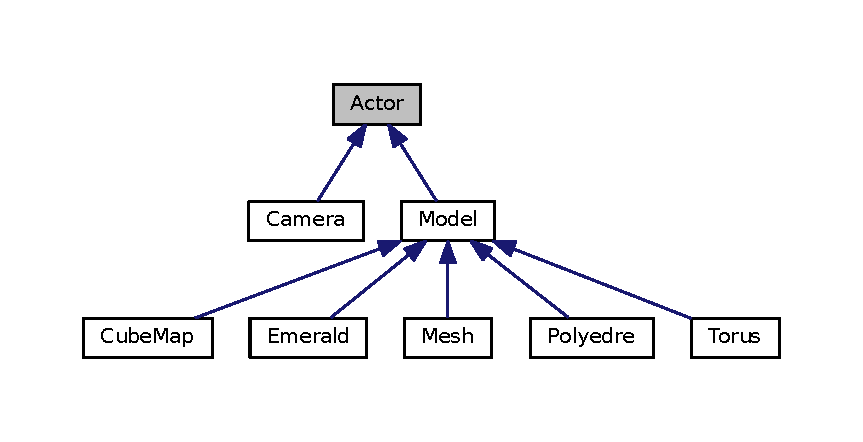
\includegraphics[width=350pt]{structActor__inherit__graph}
\end{center}
\end{figure}


\subsection{Documentation des fonctions membres}
\hypertarget{structActor_a4363e3b26c7903de41423a2fb1fc5f6e}{\index{Actor@{Actor}!update@{update}}
\index{update@{update}!Actor@{Actor}}
\subsubsection[{update}]{\setlength{\rightskip}{0pt plus 5cm}virtual void Actor\+::update (
\begin{DoxyParamCaption}
{}
\end{DoxyParamCaption}
)\hspace{0.3cm}{\ttfamily [pure virtual]}}}\label{structActor_a4363e3b26c7903de41423a2fb1fc5f6e}


Met à jour un acteur. 



Implémenté dans \hyperlink{classEmerald_ad997fe3bf39eb0556aefab1a91836895}{Emerald}, \hyperlink{classCamera_a42cda7239981a5618660d04bd5893556}{Camera}, \hyperlink{classCubeMap_af4766b5a5fafe3ce6e2cd8905b192d1c}{Cube\+Map}, \hyperlink{classPolyedre_a9ea5863ed9ee46c090e5dbafeda0ef73}{Polyedre}, \hyperlink{classModel_a4355afeacef658e098706cba1dd37118}{Model}, \hyperlink{classTorus_ac63e15f0274b1beb5e8f7f968c2ac69f}{Torus}, et \hyperlink{classMesh_abb6110295efe8ae479659e46553c952a}{Mesh}.


\hypertarget{classApplication}{\section{Référence de la classe Application}
\label{classApplication}\index{Application@{Application}}
}


{\ttfamily \#include $<$Application.\+hpp$>$}

\subsection*{Fonctions membres publiques}
\begin{DoxyCompactItemize}
\item 
std\+::shared\+\_\+ptr$<$ \hyperlink{classBaseWindow}{Base\+Window} $>$ \hyperlink{classApplication_ad4798575ca24d11794fb69ec7f1f5f84}{get\+Window} ()
\item 
std\+::shared\+\_\+ptr$<$ \hyperlink{classController}{Controller} $>$ \hyperlink{classApplication_a43268edea6339ba39334f55a7a6331e2}{get\+Controller} ()
\item 
int \hyperlink{classApplication_a9d50af9dd5d791e9e7f9236cee871dce}{run} (int=0, char $\ast$$\ast$=0)
\end{DoxyCompactItemize}
\subsection*{Fonctions membres publiques statiques}
\begin{DoxyCompactItemize}
\item 
static std\+::shared\+\_\+ptr\\*
$<$ \hyperlink{classApplication}{Application} $>$ \hyperlink{classApplication_afa5d5ce6c9369e1ea05ee6540fe07dc2}{get\+Singleton} ()
\end{DoxyCompactItemize}
\subsection*{Attributs publics statiques}
\begin{DoxyCompactItemize}
\item 
static \hyperlink{structLogger}{Logger} \hyperlink{classApplication_a1c7bdac46cde844f659892276949dca7}{Log} = \hyperlink{structLogger}{Logger}()
\end{DoxyCompactItemize}


\subsection{Description détaillée}
Cette classe gère les accès aux ressources partagées 

Définition à la ligne 19 du fichier Application.\+hpp.



Graphe d'héritage de Application\+:
\nopagebreak
\begin{figure}[H]
\begin{center}
\leavevmode
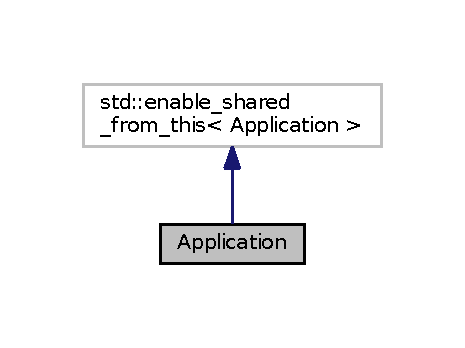
\includegraphics[width=223pt]{classApplication__inherit__graph}
\end{center}
\end{figure}


Graphe de collaboration de Application\+:
\nopagebreak
\begin{figure}[H]
\begin{center}
\leavevmode
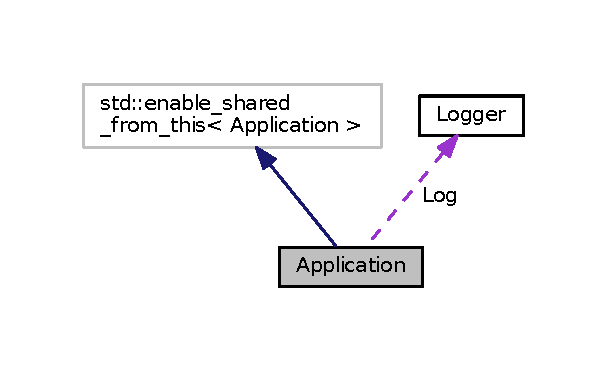
\includegraphics[width=292pt]{classApplication__coll__graph}
\end{center}
\end{figure}


\subsection{Documentation des fonctions membres}
\hypertarget{classApplication_a43268edea6339ba39334f55a7a6331e2}{\index{Application@{Application}!get\+Controller@{get\+Controller}}
\index{get\+Controller@{get\+Controller}!Application@{Application}}
\subsubsection[{get\+Controller}]{\setlength{\rightskip}{0pt plus 5cm}std\+::shared\+\_\+ptr$<${\bf Controller}$>$ Application\+::get\+Controller (
\begin{DoxyParamCaption}
{}
\end{DoxyParamCaption}
)\hspace{0.3cm}{\ttfamily [inline]}}}\label{classApplication_a43268edea6339ba39334f55a7a6331e2}
\begin{DoxyReturn}{Renvoie}
Un pointeur sur l'instance existante de la manette 
\end{DoxyReturn}


Définition à la ligne 67 du fichier Application.\+hpp.

\hypertarget{classApplication_afa5d5ce6c9369e1ea05ee6540fe07dc2}{\index{Application@{Application}!get\+Singleton@{get\+Singleton}}
\index{get\+Singleton@{get\+Singleton}!Application@{Application}}
\subsubsection[{get\+Singleton}]{\setlength{\rightskip}{0pt plus 5cm}static std\+::shared\+\_\+ptr$<${\bf Application}$>$ Application\+::get\+Singleton (
\begin{DoxyParamCaption}
{}
\end{DoxyParamCaption}
)\hspace{0.3cm}{\ttfamily [inline]}, {\ttfamily [static]}}}\label{classApplication_afa5d5ce6c9369e1ea05ee6540fe07dc2}
\begin{DoxyReturn}{Renvoie}
L'instance existante du singleton 
\end{DoxyReturn}


Définition à la ligne 55 du fichier Application.\+hpp.



Voici le graphe des appelants de cette fonction \+:
\nopagebreak
\begin{figure}[H]
\begin{center}
\leavevmode
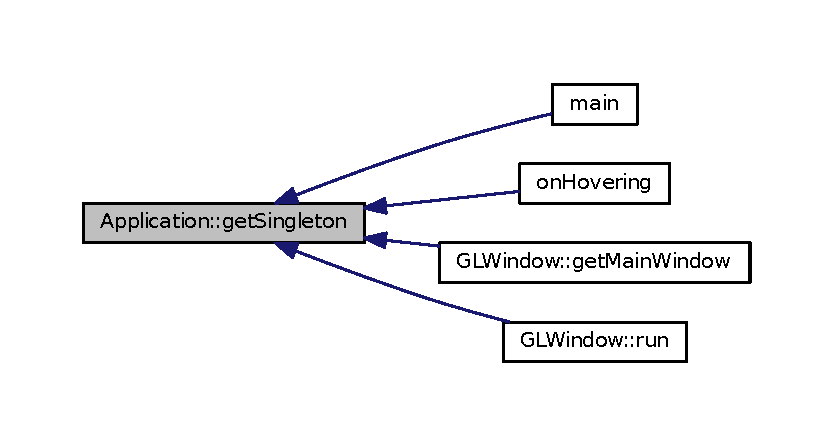
\includegraphics[width=350pt]{classApplication_afa5d5ce6c9369e1ea05ee6540fe07dc2_icgraph}
\end{center}
\end{figure}


\hypertarget{classApplication_ad4798575ca24d11794fb69ec7f1f5f84}{\index{Application@{Application}!get\+Window@{get\+Window}}
\index{get\+Window@{get\+Window}!Application@{Application}}
\subsubsection[{get\+Window}]{\setlength{\rightskip}{0pt plus 5cm}std\+::shared\+\_\+ptr$<${\bf Base\+Window}$>$ Application\+::get\+Window (
\begin{DoxyParamCaption}
{}
\end{DoxyParamCaption}
)\hspace{0.3cm}{\ttfamily [inline]}}}\label{classApplication_ad4798575ca24d11794fb69ec7f1f5f84}
\begin{DoxyReturn}{Renvoie}
Un pointeur sur l'instance existante de la fenêtre 
\end{DoxyReturn}


Définition à la ligne 59 du fichier Application.\+hpp.

\hypertarget{classApplication_a9d50af9dd5d791e9e7f9236cee871dce}{\index{Application@{Application}!run@{run}}
\index{run@{run}!Application@{Application}}
\subsubsection[{run}]{\setlength{\rightskip}{0pt plus 5cm}int Application\+::run (
\begin{DoxyParamCaption}
\item[{int}]{argc = {\ttfamily 0}, }
\item[{char $\ast$$\ast$}]{argv = {\ttfamily 0}}
\end{DoxyParamCaption}
)}}\label{classApplication_a9d50af9dd5d791e9e7f9236cee871dce}
\begin{DoxyReturn}{Renvoie}
L'état de fin d'exécution de l'application. 
\end{DoxyReturn}


Définition à la ligne 29 du fichier Application.\+cpp.



Voici le graphe d'appel pour cette fonction \+:
\nopagebreak
\begin{figure}[H]
\begin{center}
\leavevmode
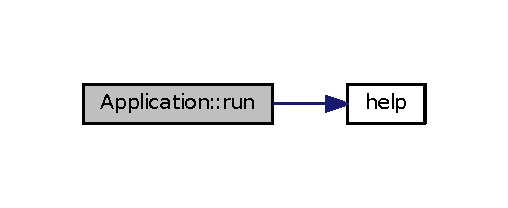
\includegraphics[width=244pt]{classApplication_a9d50af9dd5d791e9e7f9236cee871dce_cgraph}
\end{center}
\end{figure}




\subsection{Documentation des champs}
\hypertarget{classApplication_a1c7bdac46cde844f659892276949dca7}{\index{Application@{Application}!Log@{Log}}
\index{Log@{Log}!Application@{Application}}
\subsubsection[{Log}]{\setlength{\rightskip}{0pt plus 5cm}{\bf Logger} Application\+::\+Log = {\bf Logger}()\hspace{0.3cm}{\ttfamily [static]}}}\label{classApplication_a1c7bdac46cde844f659892276949dca7}
{\ttfamily Objet} utilisé pour logger 

Définition à la ligne 76 du fichier Application.\+hpp.


\hypertarget{classBaseWindow}{\section{Référence de la classe Base\+Window}
\label{classBaseWindow}\index{Base\+Window@{Base\+Window}}
}


{\ttfamily \#include $<$Base\+Window.\+hpp$>$}

\subsection*{Fonctions membres publiques}
\begin{DoxyCompactItemize}
\item 
virtual int \hyperlink{classBaseWindow_a2faf52e77b0c61225d81be8b25afd661}{run} (int=0, char $\ast$$\ast$=0)=0
\item 
virtual \hyperlink{classBaseWindow_a0095436d2c51405b0534f3c60e5fbd20}{$\sim$\+Base\+Window} ()
\end{DoxyCompactItemize}


\subsection{Description détaillée}
\begin{DoxyAuthor}{Auteur}
N.\+Boutemeur 'interface d'une fenêtre. 
\end{DoxyAuthor}


Définition à la ligne 10 du fichier Base\+Window.\+hpp.



Graphe d'héritage de Base\+Window\+:
\nopagebreak
\begin{figure}[H]
\begin{center}
\leavevmode
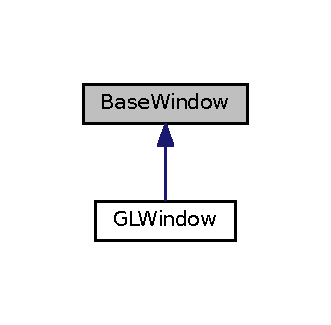
\includegraphics[width=159pt]{classBaseWindow__inherit__graph}
\end{center}
\end{figure}


\subsection{Documentation des constructeurs et destructeur}
\hypertarget{classBaseWindow_a0095436d2c51405b0534f3c60e5fbd20}{\index{Base\+Window@{Base\+Window}!````~Base\+Window@{$\sim$\+Base\+Window}}
\index{````~Base\+Window@{$\sim$\+Base\+Window}!Base\+Window@{Base\+Window}}
\subsubsection[{$\sim$\+Base\+Window}]{\setlength{\rightskip}{0pt plus 5cm}virtual Base\+Window\+::$\sim$\+Base\+Window (
\begin{DoxyParamCaption}
{}
\end{DoxyParamCaption}
)\hspace{0.3cm}{\ttfamily [inline]}, {\ttfamily [virtual]}}}\label{classBaseWindow_a0095436d2c51405b0534f3c60e5fbd20}


Définition à la ligne 17 du fichier Base\+Window.\+hpp.



\subsection{Documentation des fonctions membres}
\hypertarget{classBaseWindow_a2faf52e77b0c61225d81be8b25afd661}{\index{Base\+Window@{Base\+Window}!run@{run}}
\index{run@{run}!Base\+Window@{Base\+Window}}
\subsubsection[{run}]{\setlength{\rightskip}{0pt plus 5cm}virtual int Base\+Window\+::run (
\begin{DoxyParamCaption}
\item[{int}]{ = {\ttfamily 0}, }
\item[{char $\ast$$\ast$}]{ = {\ttfamily 0}}
\end{DoxyParamCaption}
)\hspace{0.3cm}{\ttfamily [pure virtual]}}}\label{classBaseWindow_a2faf52e77b0c61225d81be8b25afd661}
\begin{DoxyReturn}{Renvoie}
L'état d'exécution 
\end{DoxyReturn}


Implémenté dans \hyperlink{classGLWindow_a297b34b4bbf69b29516e279839262623}{G\+L\+Window}.


\hypertarget{classBetaRoom}{\section{Référence de la classe Beta\+Room}
\label{classBetaRoom}\index{Beta\+Room@{Beta\+Room}}
}


{\ttfamily \#include $<$Beta\+Room.\+hpp$>$}

\subsection*{Fonctions membres publiques}
\begin{DoxyCompactItemize}
\item 
\hyperlink{classBetaRoom_a2dbe2bd7a60336a10040604baca9f389}{Beta\+Room} ()
\item 
virtual void \hyperlink{classBetaRoom_a5ca4002697c35ee24a59d9d2ccab3e49}{render} ()
\begin{DoxyCompactList}\small\item\em Rends la scène sur la cible active. \end{DoxyCompactList}\item 
virtual \hyperlink{classBetaRoom_a03ddec958e0cfb3e9458ea68b9b5a6b7}{$\sim$\+Beta\+Room} ()
\end{DoxyCompactItemize}
\subsection*{Membres hérités additionnels}


\subsection{Description détaillée}
scène constituée de 4 objets 

Définition à la ligne 17 du fichier Beta\+Room.\+hpp.



Graphe d'héritage de Beta\+Room\+:
\nopagebreak
\begin{figure}[H]
\begin{center}
\leavevmode
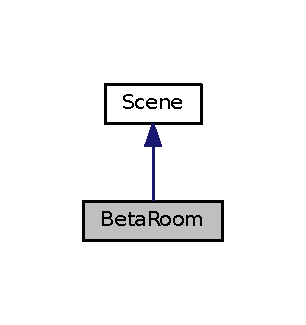
\includegraphics[width=147pt]{classBetaRoom__inherit__graph}
\end{center}
\end{figure}


Graphe de collaboration de Beta\+Room\+:
\nopagebreak
\begin{figure}[H]
\begin{center}
\leavevmode
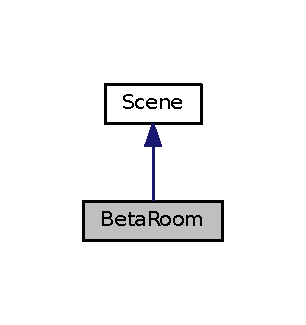
\includegraphics[width=147pt]{classBetaRoom__coll__graph}
\end{center}
\end{figure}


\subsection{Documentation des constructeurs et destructeur}
\hypertarget{classBetaRoom_a2dbe2bd7a60336a10040604baca9f389}{\index{Beta\+Room@{Beta\+Room}!Beta\+Room@{Beta\+Room}}
\index{Beta\+Room@{Beta\+Room}!Beta\+Room@{Beta\+Room}}
\subsubsection[{Beta\+Room}]{\setlength{\rightskip}{0pt plus 5cm}Beta\+Room\+::\+Beta\+Room (
\begin{DoxyParamCaption}
{}
\end{DoxyParamCaption}
)}}\label{classBetaRoom_a2dbe2bd7a60336a10040604baca9f389}

\begin{DoxyParams}{Paramètres}
{\em cam} & La caméra à utiliser pour le rendu \\
\hline
\end{DoxyParams}


Définition à la ligne 12 du fichier Beta\+Room.\+cpp.

\hypertarget{classBetaRoom_a03ddec958e0cfb3e9458ea68b9b5a6b7}{\index{Beta\+Room@{Beta\+Room}!````~Beta\+Room@{$\sim$\+Beta\+Room}}
\index{````~Beta\+Room@{$\sim$\+Beta\+Room}!Beta\+Room@{Beta\+Room}}
\subsubsection[{$\sim$\+Beta\+Room}]{\setlength{\rightskip}{0pt plus 5cm}virtual Beta\+Room\+::$\sim$\+Beta\+Room (
\begin{DoxyParamCaption}
{}
\end{DoxyParamCaption}
)\hspace{0.3cm}{\ttfamily [inline]}, {\ttfamily [virtual]}}}\label{classBetaRoom_a03ddec958e0cfb3e9458ea68b9b5a6b7}


Définition à la ligne 43 du fichier Beta\+Room.\+hpp.



\subsection{Documentation des fonctions membres}
\hypertarget{classBetaRoom_a5ca4002697c35ee24a59d9d2ccab3e49}{\index{Beta\+Room@{Beta\+Room}!render@{render}}
\index{render@{render}!Beta\+Room@{Beta\+Room}}
\subsubsection[{render}]{\setlength{\rightskip}{0pt plus 5cm}void Beta\+Room\+::render (
\begin{DoxyParamCaption}
{}
\end{DoxyParamCaption}
)\hspace{0.3cm}{\ttfamily [virtual]}}}\label{classBetaRoom_a5ca4002697c35ee24a59d9d2ccab3e49}


Rends la scène sur la cible active. 



Réimplémentée à partir de \hyperlink{classScene_a4ddf2d16f371ee9533b3faf1dd5ddfb1}{Scene}.



Définition à la ligne 31 du fichier Beta\+Room.\+cpp.



Voici le graphe d'appel pour cette fonction \+:
\nopagebreak
\begin{figure}[H]
\begin{center}
\leavevmode
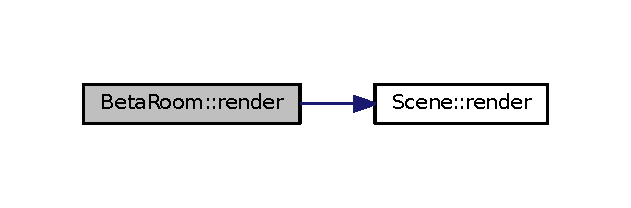
\includegraphics[width=303pt]{classBetaRoom_a5ca4002697c35ee24a59d9d2ccab3e49_cgraph}
\end{center}
\end{figure}




Voici le graphe des appelants de cette fonction \+:
\nopagebreak
\begin{figure}[H]
\begin{center}
\leavevmode
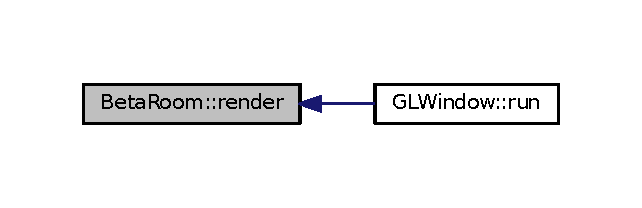
\includegraphics[width=308pt]{classBetaRoom_a5ca4002697c35ee24a59d9d2ccab3e49_icgraph}
\end{center}
\end{figure}



\hypertarget{classCamera}{\section{Référence de la classe Camera}
\label{classCamera}\index{Camera@{Camera}}
}


{\ttfamily \#include $<$Camera.\+hpp$>$}

\subsection*{Fonctions membres publiques}
\begin{DoxyCompactItemize}
\item 
\hyperlink{classCamera_a01f94c3543f56ede7af49dc778f19331}{Camera} ()
\begin{DoxyCompactList}\small\item\em Instancie une caméra, liée à une fenêtre. \end{DoxyCompactList}\item 
virtual void \hyperlink{classCamera_a42cda7239981a5618660d04bd5893556}{update} ()
\begin{DoxyCompactList}\small\item\em Mets à jour la caméra. \end{DoxyCompactList}\item 
glm\+::mat4 \hyperlink{classCamera_af16af4b8b0ff1e4381359ecd2075092d}{get\+View} () const 
\begin{DoxyCompactList}\small\item\em Renvoie une copie de la matrice de vue. \end{DoxyCompactList}\item 
glm\+::mat4 \hyperlink{classCamera_aa3bc85ea7125f9051a45cb522dee71ff}{get\+Projection} () const 
\begin{DoxyCompactList}\small\item\em Renvoie une copie de la matrice de projection. \end{DoxyCompactList}\item 
glm\+::vec3 \hyperlink{classCamera_ad741cb975e8ea88698ed1b0216a0bb82}{get\+Position} () const 
\begin{DoxyCompactList}\small\item\em Renvoie la position de la caméra. \end{DoxyCompactList}\end{DoxyCompactItemize}
\subsection*{Champs de données}
\begin{DoxyCompactItemize}
\item 
std\+::shared\+\_\+ptr$<$ \hyperlink{classController}{Controller} $>$ \hyperlink{classCamera_a879e38247f44c717796f38a501d335e3}{m\+\_\+controller}
\item 
glm\+::vec3 \hyperlink{classCamera_a2674b50120e3bafbab54b53e4313d54d}{m\+\_\+position}
\item 
glm\+::vec3 \hyperlink{classCamera_a64d1bf3cfff83eeb294a6cf53a0d4255}{m\+\_\+direction}
\item 
\hyperlink{classGLWindow}{G\+L\+Window} $\ast$ \hyperlink{classCamera_a97abe5fea87690fbb00d920ecf5fcce8}{m\+\_\+gl\+Win}
\item 
glm\+::mat4 \hyperlink{classCamera_ad86d990f179df0cd5560bca660d5ffbf}{m\+\_\+view}
\end{DoxyCompactItemize}
\subsection*{Amis}
\begin{DoxyCompactItemize}
\item 
void \hyperlink{classCamera_ae67f6cdba1f3601ad8cf82996105fe76}{on\+Hovering} (G\+L\+F\+Wwindow $\ast$, double, double)
\end{DoxyCompactItemize}


\subsection{Description détaillée}
caméra dans l'espace 

Définition à la ligne 21 du fichier Camera.\+hpp.



Graphe d'héritage de Camera\+:
\nopagebreak
\begin{figure}[H]
\begin{center}
\leavevmode
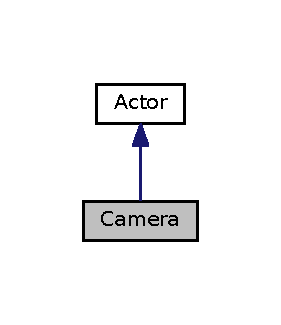
\includegraphics[width=135pt]{classCamera__inherit__graph}
\end{center}
\end{figure}


Graphe de collaboration de Camera\+:
\nopagebreak
\begin{figure}[H]
\begin{center}
\leavevmode
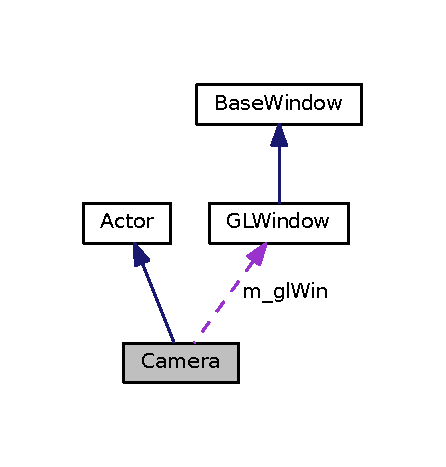
\includegraphics[width=214pt]{classCamera__coll__graph}
\end{center}
\end{figure}


\subsection{Documentation des constructeurs et destructeur}
\hypertarget{classCamera_a01f94c3543f56ede7af49dc778f19331}{\index{Camera@{Camera}!Camera@{Camera}}
\index{Camera@{Camera}!Camera@{Camera}}
\subsubsection[{Camera}]{\setlength{\rightskip}{0pt plus 5cm}Camera\+::\+Camera (
\begin{DoxyParamCaption}
{}
\end{DoxyParamCaption}
)}}\label{classCamera_a01f94c3543f56ede7af49dc778f19331}


Instancie une caméra, liée à une fenêtre. 



Définition à la ligne 41 du fichier Camera.\+cpp.



\subsection{Documentation des fonctions membres}
\hypertarget{classCamera_ad741cb975e8ea88698ed1b0216a0bb82}{\index{Camera@{Camera}!get\+Position@{get\+Position}}
\index{get\+Position@{get\+Position}!Camera@{Camera}}
\subsubsection[{get\+Position}]{\setlength{\rightskip}{0pt plus 5cm}glm\+::vec3 Camera\+::get\+Position (
\begin{DoxyParamCaption}
{}
\end{DoxyParamCaption}
) const\hspace{0.3cm}{\ttfamily [inline]}}}\label{classCamera_ad741cb975e8ea88698ed1b0216a0bb82}


Renvoie la position de la caméra. 



Définition à la ligne 64 du fichier Camera.\+hpp.



Voici le graphe des appelants de cette fonction \+:
\nopagebreak
\begin{figure}[H]
\begin{center}
\leavevmode
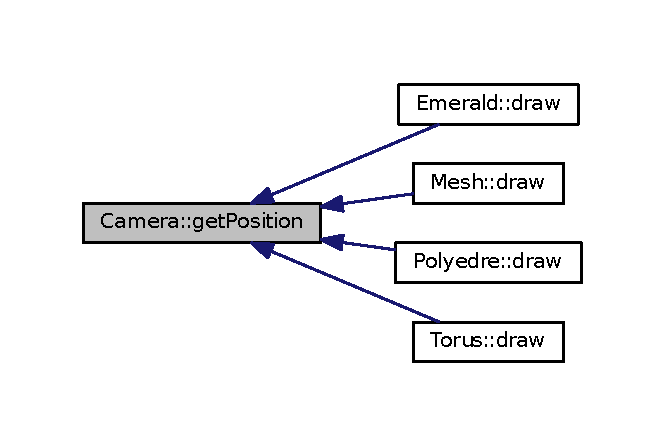
\includegraphics[width=319pt]{classCamera_ad741cb975e8ea88698ed1b0216a0bb82_icgraph}
\end{center}
\end{figure}


\hypertarget{classCamera_aa3bc85ea7125f9051a45cb522dee71ff}{\index{Camera@{Camera}!get\+Projection@{get\+Projection}}
\index{get\+Projection@{get\+Projection}!Camera@{Camera}}
\subsubsection[{get\+Projection}]{\setlength{\rightskip}{0pt plus 5cm}glm\+::mat4 Camera\+::get\+Projection (
\begin{DoxyParamCaption}
{}
\end{DoxyParamCaption}
) const\hspace{0.3cm}{\ttfamily [inline]}}}\label{classCamera_aa3bc85ea7125f9051a45cb522dee71ff}


Renvoie une copie de la matrice de projection. 



Définition à la ligne 60 du fichier Camera.\+hpp.



Voici le graphe des appelants de cette fonction \+:
\nopagebreak
\begin{figure}[H]
\begin{center}
\leavevmode
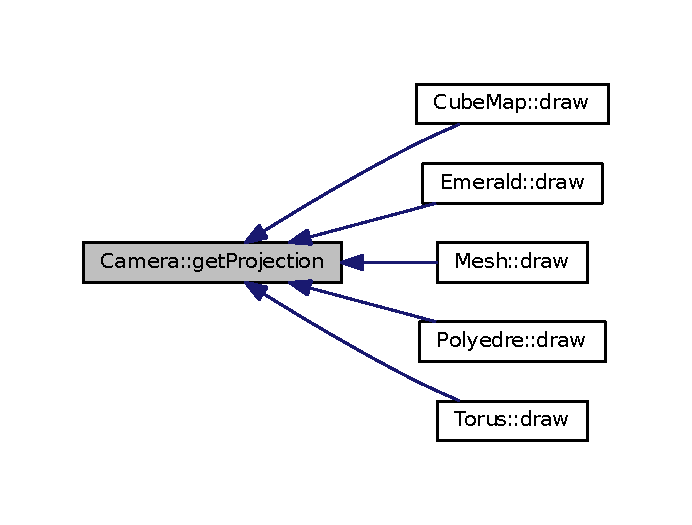
\includegraphics[width=332pt]{classCamera_aa3bc85ea7125f9051a45cb522dee71ff_icgraph}
\end{center}
\end{figure}


\hypertarget{classCamera_af16af4b8b0ff1e4381359ecd2075092d}{\index{Camera@{Camera}!get\+View@{get\+View}}
\index{get\+View@{get\+View}!Camera@{Camera}}
\subsubsection[{get\+View}]{\setlength{\rightskip}{0pt plus 5cm}glm\+::mat4 Camera\+::get\+View (
\begin{DoxyParamCaption}
{}
\end{DoxyParamCaption}
) const\hspace{0.3cm}{\ttfamily [inline]}}}\label{classCamera_af16af4b8b0ff1e4381359ecd2075092d}


Renvoie une copie de la matrice de vue. 

\begin{DoxyRefDesc}{Obsolète}
\item[\hyperlink{deprecated__deprecated000001}{Obsolète}]Utilisez m\+\_\+view plutôt \end{DoxyRefDesc}


Définition à la ligne 56 du fichier Camera.\+hpp.



Voici le graphe des appelants de cette fonction \+:
\nopagebreak
\begin{figure}[H]
\begin{center}
\leavevmode
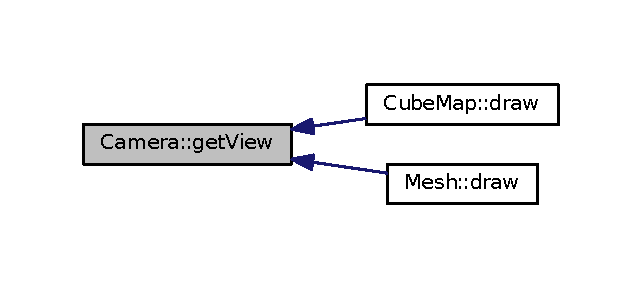
\includegraphics[width=308pt]{classCamera_af16af4b8b0ff1e4381359ecd2075092d_icgraph}
\end{center}
\end{figure}


\hypertarget{classCamera_a42cda7239981a5618660d04bd5893556}{\index{Camera@{Camera}!update@{update}}
\index{update@{update}!Camera@{Camera}}
\subsubsection[{update}]{\setlength{\rightskip}{0pt plus 5cm}void Camera\+::update (
\begin{DoxyParamCaption}
{}
\end{DoxyParamCaption}
)\hspace{0.3cm}{\ttfamily [virtual]}}}\label{classCamera_a42cda7239981a5618660d04bd5893556}


Mets à jour la caméra. 



Implémente \hyperlink{structActor_a4363e3b26c7903de41423a2fb1fc5f6e}{Actor}.



Définition à la ligne 55 du fichier Camera.\+cpp.



\subsection{Documentation des fonctions amies et associées}
\hypertarget{classCamera_ae67f6cdba1f3601ad8cf82996105fe76}{\index{Camera@{Camera}!on\+Hovering@{on\+Hovering}}
\index{on\+Hovering@{on\+Hovering}!Camera@{Camera}}
\subsubsection[{on\+Hovering}]{\setlength{\rightskip}{0pt plus 5cm}void on\+Hovering (
\begin{DoxyParamCaption}
\item[{G\+L\+F\+Wwindow $\ast$}]{win, }
\item[{double}]{x, }
\item[{double}]{y}
\end{DoxyParamCaption}
)\hspace{0.3cm}{\ttfamily [friend]}}}\label{classCamera_ae67f6cdba1f3601ad8cf82996105fe76}


Définition à la ligne 15 du fichier Camera.\+cpp.



\subsection{Documentation des champs}
\hypertarget{classCamera_a879e38247f44c717796f38a501d335e3}{\index{Camera@{Camera}!m\+\_\+controller@{m\+\_\+controller}}
\index{m\+\_\+controller@{m\+\_\+controller}!Camera@{Camera}}
\subsubsection[{m\+\_\+controller}]{\setlength{\rightskip}{0pt plus 5cm}Camera\+::m\+\_\+controller}}\label{classCamera_a879e38247f44c717796f38a501d335e3}
{\ttfamily Pointe} sur l'instance existante de la manette 

Définition à la ligne 51 du fichier Camera.\+hpp.

\hypertarget{classCamera_a64d1bf3cfff83eeb294a6cf53a0d4255}{\index{Camera@{Camera}!m\+\_\+direction@{m\+\_\+direction}}
\index{m\+\_\+direction@{m\+\_\+direction}!Camera@{Camera}}
\subsubsection[{m\+\_\+direction}]{\setlength{\rightskip}{0pt plus 5cm}Camera\+::m\+\_\+direction}}\label{classCamera_a64d1bf3cfff83eeb294a6cf53a0d4255}
{\ttfamily Direction} dans laquelle regarde la caméra 

Définition à la ligne 73 du fichier Camera.\+hpp.

\hypertarget{classCamera_a97abe5fea87690fbb00d920ecf5fcce8}{\index{Camera@{Camera}!m\+\_\+gl\+Win@{m\+\_\+gl\+Win}}
\index{m\+\_\+gl\+Win@{m\+\_\+gl\+Win}!Camera@{Camera}}
\subsubsection[{m\+\_\+gl\+Win}]{\setlength{\rightskip}{0pt plus 5cm}Camera\+::m\+\_\+gl\+Win}}\label{classCamera_a97abe5fea87690fbb00d920ecf5fcce8}
{\ttfamily Pointeur} vers l'unique instance de la fenêtre 

Définition à la ligne 78 du fichier Camera.\+hpp.

\hypertarget{classCamera_a2674b50120e3bafbab54b53e4313d54d}{\index{Camera@{Camera}!m\+\_\+position@{m\+\_\+position}}
\index{m\+\_\+position@{m\+\_\+position}!Camera@{Camera}}
\subsubsection[{m\+\_\+position}]{\setlength{\rightskip}{0pt plus 5cm}Camera\+::m\+\_\+position}}\label{classCamera_a2674b50120e3bafbab54b53e4313d54d}
{\ttfamily Position} de la caméra dans le monde 

Définition à la ligne 73 du fichier Camera.\+hpp.

\hypertarget{classCamera_ad86d990f179df0cd5560bca660d5ffbf}{\index{Camera@{Camera}!m\+\_\+view@{m\+\_\+view}}
\index{m\+\_\+view@{m\+\_\+view}!Camera@{Camera}}
\subsubsection[{m\+\_\+view}]{\setlength{\rightskip}{0pt plus 5cm}Camera\+::m\+\_\+view}}\label{classCamera_ad86d990f179df0cd5560bca660d5ffbf}
{\ttfamily Matrice} de vue de la caméra 

Définition à la ligne 83 du fichier Camera.\+hpp.


\hypertarget{classController}{\section{Référence de la classe Controller}
\label{classController}\index{Controller@{Controller}}
}


{\ttfamily \#include $<$Controller.\+hpp$>$}

\subsection*{Fonctions membres publiques}
\begin{DoxyCompactItemize}
\item 
virtual glm\+::vec2 \hyperlink{classController_a7436ccdad4f8dae40d61bf47b262191b}{get\+Main\+Stick\+Position} ()=0
\item 
virtual glm\+::vec2 \hyperlink{classController_ad48cb8e46282bdb3f7cd1178944eb45c}{get\+Secondary\+Stick\+Position} ()=0
\item 
virtual glm\+::vec2 \hyperlink{classController_ad98f33e8f7dfe9015eb8883d3881e373}{get\+Triggers} ()=0
\item 
virtual std\+::vector$<$ bool $>$ \hyperlink{classController_af7483fe863ff38bd2e9617771c450931}{get\+Buttons} ()=0
\item 
virtual \hyperlink{classController_a867c1b386aa6e63d986a01ddaeccea5a}{$\sim$\+Controller} ()
\end{DoxyCompactItemize}


\subsection{Description détaillée}
\hyperlink{classController}{Controller} définie les caractéristiques d'une manette 

Définition à la ligne 18 du fichier Controller.\+hpp.



Graphe d'héritage de Controller\+:
\nopagebreak
\begin{figure}[H]
\begin{center}
\leavevmode
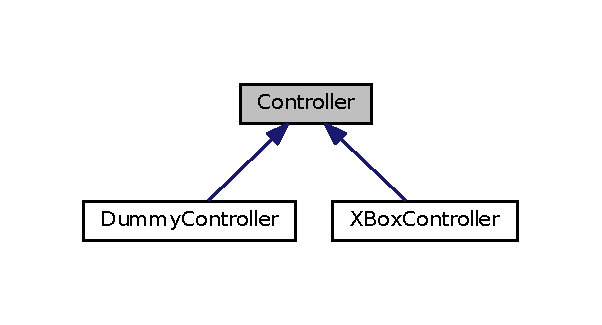
\includegraphics[width=289pt]{classController__inherit__graph}
\end{center}
\end{figure}


\subsection{Documentation des constructeurs et destructeur}
\hypertarget{classController_a867c1b386aa6e63d986a01ddaeccea5a}{\index{Controller@{Controller}!````~Controller@{$\sim$\+Controller}}
\index{````~Controller@{$\sim$\+Controller}!Controller@{Controller}}
\subsubsection[{$\sim$\+Controller}]{\setlength{\rightskip}{0pt plus 5cm}virtual Controller\+::$\sim$\+Controller (
\begin{DoxyParamCaption}
{}
\end{DoxyParamCaption}
)\hspace{0.3cm}{\ttfamily [inline]}, {\ttfamily [virtual]}}}\label{classController_a867c1b386aa6e63d986a01ddaeccea5a}


Définition à la ligne 43 du fichier Controller.\+hpp.



\subsection{Documentation des fonctions membres}
\hypertarget{classController_af7483fe863ff38bd2e9617771c450931}{\index{Controller@{Controller}!get\+Buttons@{get\+Buttons}}
\index{get\+Buttons@{get\+Buttons}!Controller@{Controller}}
\subsubsection[{get\+Buttons}]{\setlength{\rightskip}{0pt plus 5cm}virtual std\+::vector$<$bool$>$ Controller\+::get\+Buttons (
\begin{DoxyParamCaption}
{}
\end{DoxyParamCaption}
)\hspace{0.3cm}{\ttfamily [pure virtual]}}}\label{classController_af7483fe863ff38bd2e9617771c450931}
\begin{DoxyReturn}{Renvoie}
Les boutons pressés 
\end{DoxyReturn}


Implémenté dans \hyperlink{classXBoxController_a7f2177c57462c0f488986affcd7e8811}{X\+Box\+Controller}, et \hyperlink{structDummyController_af19894dd92abd6a975f48759c524c232}{Dummy\+Controller}.

\hypertarget{classController_a7436ccdad4f8dae40d61bf47b262191b}{\index{Controller@{Controller}!get\+Main\+Stick\+Position@{get\+Main\+Stick\+Position}}
\index{get\+Main\+Stick\+Position@{get\+Main\+Stick\+Position}!Controller@{Controller}}
\subsubsection[{get\+Main\+Stick\+Position}]{\setlength{\rightskip}{0pt plus 5cm}virtual glm\+::vec2 Controller\+::get\+Main\+Stick\+Position (
\begin{DoxyParamCaption}
{}
\end{DoxyParamCaption}
)\hspace{0.3cm}{\ttfamily [pure virtual]}}}\label{classController_a7436ccdad4f8dae40d61bf47b262191b}
\begin{DoxyReturn}{Renvoie}
La position du stick principal, les 2 axes dans l'interval \mbox{[}-\/1; 1\mbox{]} 
\end{DoxyReturn}


Implémenté dans \hyperlink{classXBoxController_adec21f77b6380856458c5e991c2d2805}{X\+Box\+Controller}, et \hyperlink{structDummyController_a0f91702b184d73e7c5e1e9a54cee1f48}{Dummy\+Controller}.

\hypertarget{classController_ad48cb8e46282bdb3f7cd1178944eb45c}{\index{Controller@{Controller}!get\+Secondary\+Stick\+Position@{get\+Secondary\+Stick\+Position}}
\index{get\+Secondary\+Stick\+Position@{get\+Secondary\+Stick\+Position}!Controller@{Controller}}
\subsubsection[{get\+Secondary\+Stick\+Position}]{\setlength{\rightskip}{0pt plus 5cm}virtual glm\+::vec2 Controller\+::get\+Secondary\+Stick\+Position (
\begin{DoxyParamCaption}
{}
\end{DoxyParamCaption}
)\hspace{0.3cm}{\ttfamily [pure virtual]}}}\label{classController_ad48cb8e46282bdb3f7cd1178944eb45c}
\begin{DoxyReturn}{Renvoie}
La position du stick secondaire, les 2 axes dans l'interval \mbox{[}-\/1; 1\mbox{]} 
\end{DoxyReturn}


Implémenté dans \hyperlink{classXBoxController_a6fe09f7fe9cc8439a909cbf45cdcaafd}{X\+Box\+Controller}, et \hyperlink{structDummyController_a9475640a5f1678c556c718c1cc84b589}{Dummy\+Controller}.

\hypertarget{classController_ad98f33e8f7dfe9015eb8883d3881e373}{\index{Controller@{Controller}!get\+Triggers@{get\+Triggers}}
\index{get\+Triggers@{get\+Triggers}!Controller@{Controller}}
\subsubsection[{get\+Triggers}]{\setlength{\rightskip}{0pt plus 5cm}virtual glm\+::vec2 Controller\+::get\+Triggers (
\begin{DoxyParamCaption}
{}
\end{DoxyParamCaption}
)\hspace{0.3cm}{\ttfamily [pure virtual]}}}\label{classController_ad98f33e8f7dfe9015eb8883d3881e373}
\begin{DoxyReturn}{Renvoie}
La position des gâchettes, les 2 axes dans l'interval \mbox{[}-\/1; 1\mbox{]} 
\end{DoxyReturn}


Implémenté dans \hyperlink{classXBoxController_a3b3cf6e2302e80423f5ffe060cf502db}{X\+Box\+Controller}, et \hyperlink{structDummyController_af8f0e6203fbc4204195c72a5675c981e}{Dummy\+Controller}.


\hypertarget{classCubeMap}{\section{Référence de la classe Cube\+Map}
\label{classCubeMap}\index{Cube\+Map@{Cube\+Map}}
}


{\ttfamily \#include $<$Cube\+Map.\+hpp$>$}

\subsection*{Fonctions membres publiques}
\begin{DoxyCompactItemize}
\item 
\hyperlink{classCubeMap_ac33e45b385642ae69ab71e7d6842599f}{Cube\+Map} ()
\begin{DoxyCompactList}\small\item\em Instancie une skybox. \end{DoxyCompactList}\item 
virtual void \hyperlink{classCubeMap_a9e042ac0b15cf9a28af3320b769f140f}{draw} (const \hyperlink{classCamera}{Camera} \&)
\begin{DoxyCompactList}\small\item\em dessine la skybox \end{DoxyCompactList}\item 
virtual void \hyperlink{classCubeMap_af4766b5a5fafe3ce6e2cd8905b192d1c}{update} ()
\begin{DoxyCompactList}\small\item\em met a jour une skybox \end{DoxyCompactList}\item 
unsigned \hyperlink{classCubeMap_ac59d8de964ee64abd3c112cf5b62e73c}{get\+Env\+Texture} ()
\begin{DoxyCompactList}\small\item\em Récupère l'identifiant de la texture utilisée. \end{DoxyCompactList}\end{DoxyCompactItemize}
\subsection*{Membres hérités additionnels}


\subsection{Description détaillée}
qui englobe une scène. 

Définition à la ligne 13 du fichier Cube\+Map.\+hpp.



Graphe d'héritage de Cube\+Map\+:
\nopagebreak
\begin{figure}[H]
\begin{center}
\leavevmode
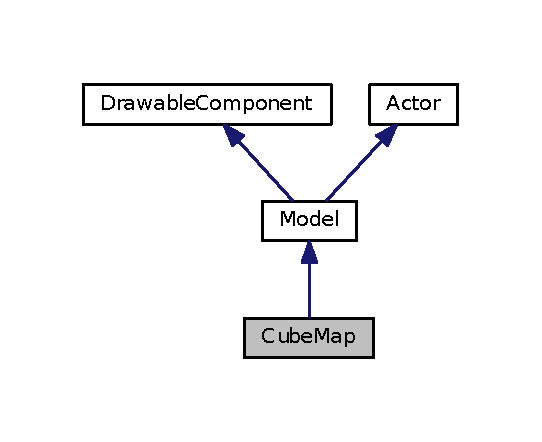
\includegraphics[width=260pt]{classCubeMap__inherit__graph}
\end{center}
\end{figure}


Graphe de collaboration de Cube\+Map\+:
\nopagebreak
\begin{figure}[H]
\begin{center}
\leavevmode
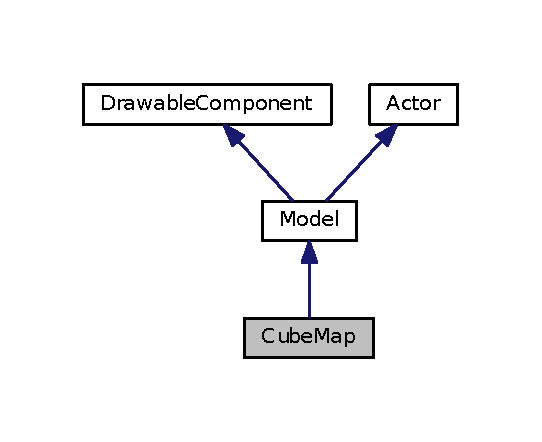
\includegraphics[width=260pt]{classCubeMap__coll__graph}
\end{center}
\end{figure}


\subsection{Documentation des constructeurs et destructeur}
\hypertarget{classCubeMap_ac33e45b385642ae69ab71e7d6842599f}{\index{Cube\+Map@{Cube\+Map}!Cube\+Map@{Cube\+Map}}
\index{Cube\+Map@{Cube\+Map}!Cube\+Map@{Cube\+Map}}
\subsubsection[{Cube\+Map}]{\setlength{\rightskip}{0pt plus 5cm}Cube\+Map\+::\+Cube\+Map (
\begin{DoxyParamCaption}
{}
\end{DoxyParamCaption}
)}}\label{classCubeMap_ac33e45b385642ae69ab71e7d6842599f}


Instancie une skybox. 



Définition à la ligne 14 du fichier Cube\+Map.\+cpp.



\subsection{Documentation des fonctions membres}
\hypertarget{classCubeMap_a9e042ac0b15cf9a28af3320b769f140f}{\index{Cube\+Map@{Cube\+Map}!draw@{draw}}
\index{draw@{draw}!Cube\+Map@{Cube\+Map}}
\subsubsection[{draw}]{\setlength{\rightskip}{0pt plus 5cm}void Cube\+Map\+::draw (
\begin{DoxyParamCaption}
\item[{const {\bf Camera} \&}]{cam}
\end{DoxyParamCaption}
)\hspace{0.3cm}{\ttfamily [virtual]}}}\label{classCubeMap_a9e042ac0b15cf9a28af3320b769f140f}


dessine la skybox 



Implémente \hyperlink{classModel_a7df7bb611f0503bc01946fff87b68fba}{Model}.



Définition à la ligne 57 du fichier Cube\+Map.\+cpp.



Voici le graphe d'appel pour cette fonction \+:
\nopagebreak
\begin{figure}[H]
\begin{center}
\leavevmode
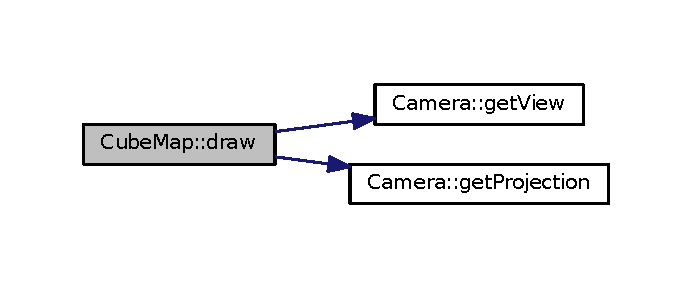
\includegraphics[width=332pt]{classCubeMap_a9e042ac0b15cf9a28af3320b769f140f_cgraph}
\end{center}
\end{figure}


\hypertarget{classCubeMap_ac59d8de964ee64abd3c112cf5b62e73c}{\index{Cube\+Map@{Cube\+Map}!get\+Env\+Texture@{get\+Env\+Texture}}
\index{get\+Env\+Texture@{get\+Env\+Texture}!Cube\+Map@{Cube\+Map}}
\subsubsection[{get\+Env\+Texture}]{\setlength{\rightskip}{0pt plus 5cm}unsigned Cube\+Map\+::get\+Env\+Texture (
\begin{DoxyParamCaption}
{}
\end{DoxyParamCaption}
)\hspace{0.3cm}{\ttfamily [inline]}}}\label{classCubeMap_ac59d8de964ee64abd3c112cf5b62e73c}


Récupère l'identifiant de la texture utilisée. 

\begin{DoxyReturn}{Renvoie}
la texture d'environnement 
\end{DoxyReturn}


Définition à la ligne 43 du fichier Cube\+Map.\+hpp.

\hypertarget{classCubeMap_af4766b5a5fafe3ce6e2cd8905b192d1c}{\index{Cube\+Map@{Cube\+Map}!update@{update}}
\index{update@{update}!Cube\+Map@{Cube\+Map}}
\subsubsection[{update}]{\setlength{\rightskip}{0pt plus 5cm}virtual void Cube\+Map\+::update (
\begin{DoxyParamCaption}
{}
\end{DoxyParamCaption}
)\hspace{0.3cm}{\ttfamily [inline]}, {\ttfamily [virtual]}}}\label{classCubeMap_af4766b5a5fafe3ce6e2cd8905b192d1c}


met a jour une skybox 



Implémente \hyperlink{classModel_a4355afeacef658e098706cba1dd37118}{Model}.



Définition à la ligne 38 du fichier Cube\+Map.\+hpp.


\hypertarget{structDrawableComponent}{\section{Référence de la structure Drawable\+Component}
\label{structDrawableComponent}\index{Drawable\+Component@{Drawable\+Component}}
}


{\ttfamily \#include $<$Drawable\+Component.\+hpp$>$}

\subsection*{Fonctions membres publiques}
\begin{DoxyCompactItemize}
\item 
virtual void \hyperlink{structDrawableComponent_ad1b6696a0f1ab135c9b2109450c75928}{draw} (const \hyperlink{classCamera}{Camera} \&)=0
\begin{DoxyCompactList}\small\item\em Dessine un objet sur la cible active. \end{DoxyCompactList}\item 
virtual \hyperlink{structDrawableComponent_a863e438d8d013b21dc44fcc38a89ca66}{$\sim$\+Drawable\+Component} ()
\end{DoxyCompactItemize}


\subsection{Description détaillée}
La classe Drawing\+Component défini des objets qui peuvent être dessinés 

Définition à la ligne 13 du fichier Drawable\+Component.\+hpp.



Graphe d'héritage de Drawable\+Component\+:
\nopagebreak
\begin{figure}[H]
\begin{center}
\leavevmode
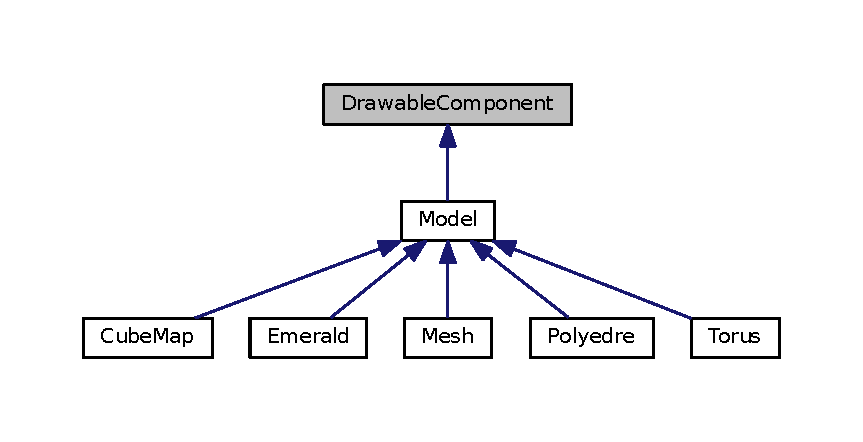
\includegraphics[width=350pt]{structDrawableComponent__inherit__graph}
\end{center}
\end{figure}


\subsection{Documentation des constructeurs et destructeur}
\hypertarget{structDrawableComponent_a863e438d8d013b21dc44fcc38a89ca66}{\index{Drawable\+Component@{Drawable\+Component}!````~Drawable\+Component@{$\sim$\+Drawable\+Component}}
\index{````~Drawable\+Component@{$\sim$\+Drawable\+Component}!Drawable\+Component@{Drawable\+Component}}
\subsubsection[{$\sim$\+Drawable\+Component}]{\setlength{\rightskip}{0pt plus 5cm}virtual Drawable\+Component\+::$\sim$\+Drawable\+Component (
\begin{DoxyParamCaption}
{}
\end{DoxyParamCaption}
)\hspace{0.3cm}{\ttfamily [inline]}, {\ttfamily [virtual]}}}\label{structDrawableComponent_a863e438d8d013b21dc44fcc38a89ca66}


Définition à la ligne 19 du fichier Drawable\+Component.\+hpp.



\subsection{Documentation des fonctions membres}
\hypertarget{structDrawableComponent_ad1b6696a0f1ab135c9b2109450c75928}{\index{Drawable\+Component@{Drawable\+Component}!draw@{draw}}
\index{draw@{draw}!Drawable\+Component@{Drawable\+Component}}
\subsubsection[{draw}]{\setlength{\rightskip}{0pt plus 5cm}virtual void Drawable\+Component\+::draw (
\begin{DoxyParamCaption}
\item[{const {\bf Camera} \&}]{}
\end{DoxyParamCaption}
)\hspace{0.3cm}{\ttfamily [pure virtual]}}}\label{structDrawableComponent_ad1b6696a0f1ab135c9b2109450c75928}


Dessine un objet sur la cible active. 



Implémenté dans \hyperlink{classEmerald_ae913346e203ed9a8115d890bd662ea41}{Emerald}, \hyperlink{classCubeMap_a9e042ac0b15cf9a28af3320b769f140f}{Cube\+Map}, \hyperlink{classPolyedre_a57ffd7e5fbba07e8b9c9737a4507a37b}{Polyedre}, \hyperlink{classModel_a7df7bb611f0503bc01946fff87b68fba}{Model}, \hyperlink{classTorus_a4d7971c04def3d60c37b1018560dcfb2}{Torus}, et \hyperlink{classMesh_aeb4e185f5d443690132b8e88bf5c669c}{Mesh}.


\hypertarget{structDummyController}{\section{Référence de la classe Dummy\+Controller}
\label{structDummyController}\index{Dummy\+Controller@{Dummy\+Controller}}
}


{\ttfamily \#include $<$Dummy\+Controller.\+hpp$>$}

\subsection*{Fonctions membres publiques}
\begin{DoxyCompactItemize}
\item 
virtual glm\+::vec2 \hyperlink{structDummyController_a0f91702b184d73e7c5e1e9a54cee1f48}{get\+Main\+Stick\+Position} () finaloverride
\item 
virtual glm\+::vec2 \hyperlink{structDummyController_a9475640a5f1678c556c718c1cc84b589}{get\+Secondary\+Stick\+Position} () finaloverride
\item 
virtual glm\+::vec2 \hyperlink{structDummyController_af8f0e6203fbc4204195c72a5675c981e}{get\+Triggers} () finaloverride
\item 
virtual std\+::vector$<$ bool $>$ \hyperlink{structDummyController_af19894dd92abd6a975f48759c524c232}{get\+Buttons} () finaloverride
\item 
virtual \hyperlink{structDummyController_a0b2f85a21ef6b0f95d608f8951541613}{$\sim$\+Dummy\+Controller} () finaloverride
\end{DoxyCompactItemize}


\subsection{Description détaillée}
\begin{DoxyAuthor}{Auteur}
N.\+Boutemeur
\end{DoxyAuthor}
Une manette qui ne fait jamais rien. 

Définition à la ligne 13 du fichier Dummy\+Controller.\+hpp.



Graphe d'héritage de Dummy\+Controller\+:
\nopagebreak
\begin{figure}[H]
\begin{center}
\leavevmode
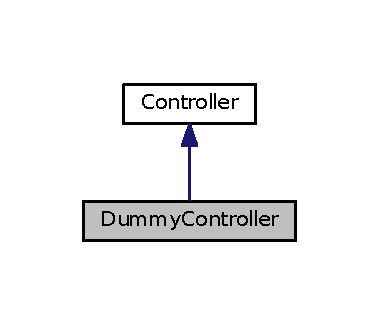
\includegraphics[width=182pt]{structDummyController__inherit__graph}
\end{center}
\end{figure}


Graphe de collaboration de Dummy\+Controller\+:
\nopagebreak
\begin{figure}[H]
\begin{center}
\leavevmode
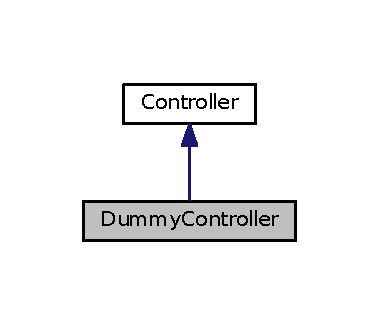
\includegraphics[width=182pt]{structDummyController__coll__graph}
\end{center}
\end{figure}


\subsection{Documentation des constructeurs et destructeur}
\hypertarget{structDummyController_a0b2f85a21ef6b0f95d608f8951541613}{\index{Dummy\+Controller@{Dummy\+Controller}!````~Dummy\+Controller@{$\sim$\+Dummy\+Controller}}
\index{````~Dummy\+Controller@{$\sim$\+Dummy\+Controller}!Dummy\+Controller@{Dummy\+Controller}}
\subsubsection[{$\sim$\+Dummy\+Controller}]{\setlength{\rightskip}{0pt plus 5cm}virtual Dummy\+Controller\+::$\sim$\+Dummy\+Controller (
\begin{DoxyParamCaption}
{}
\end{DoxyParamCaption}
)\hspace{0.3cm}{\ttfamily [inline]}, {\ttfamily [final]}, {\ttfamily [override]}, {\ttfamily [virtual]}}}\label{structDummyController_a0b2f85a21ef6b0f95d608f8951541613}


Définition à la ligne 31 du fichier Dummy\+Controller.\+hpp.



\subsection{Documentation des fonctions membres}
\hypertarget{structDummyController_af19894dd92abd6a975f48759c524c232}{\index{Dummy\+Controller@{Dummy\+Controller}!get\+Buttons@{get\+Buttons}}
\index{get\+Buttons@{get\+Buttons}!Dummy\+Controller@{Dummy\+Controller}}
\subsubsection[{get\+Buttons}]{\setlength{\rightskip}{0pt plus 5cm}virtual std\+::vector$<$bool$>$ Dummy\+Controller\+::get\+Buttons (
\begin{DoxyParamCaption}
{}
\end{DoxyParamCaption}
)\hspace{0.3cm}{\ttfamily [inline]}, {\ttfamily [final]}, {\ttfamily [override]}, {\ttfamily [virtual]}}}\label{structDummyController_af19894dd92abd6a975f48759c524c232}
\begin{DoxyReturn}{Renvoie}
Les boutons pressés 
\end{DoxyReturn}


Implémente \hyperlink{classController_af7483fe863ff38bd2e9617771c450931}{Controller}.



Définition à la ligne 30 du fichier Dummy\+Controller.\+hpp.

\hypertarget{structDummyController_a0f91702b184d73e7c5e1e9a54cee1f48}{\index{Dummy\+Controller@{Dummy\+Controller}!get\+Main\+Stick\+Position@{get\+Main\+Stick\+Position}}
\index{get\+Main\+Stick\+Position@{get\+Main\+Stick\+Position}!Dummy\+Controller@{Dummy\+Controller}}
\subsubsection[{get\+Main\+Stick\+Position}]{\setlength{\rightskip}{0pt plus 5cm}virtual glm\+::vec2 Dummy\+Controller\+::get\+Main\+Stick\+Position (
\begin{DoxyParamCaption}
{}
\end{DoxyParamCaption}
)\hspace{0.3cm}{\ttfamily [inline]}, {\ttfamily [final]}, {\ttfamily [override]}, {\ttfamily [virtual]}}}\label{structDummyController_a0f91702b184d73e7c5e1e9a54cee1f48}
\begin{DoxyReturn}{Renvoie}
La position du stick principal, les 2 axes dans l'interval \mbox{[}-\/1; 1\mbox{]} 
\end{DoxyReturn}


Implémente \hyperlink{classController_a7436ccdad4f8dae40d61bf47b262191b}{Controller}.



Définition à la ligne 18 du fichier Dummy\+Controller.\+hpp.

\hypertarget{structDummyController_a9475640a5f1678c556c718c1cc84b589}{\index{Dummy\+Controller@{Dummy\+Controller}!get\+Secondary\+Stick\+Position@{get\+Secondary\+Stick\+Position}}
\index{get\+Secondary\+Stick\+Position@{get\+Secondary\+Stick\+Position}!Dummy\+Controller@{Dummy\+Controller}}
\subsubsection[{get\+Secondary\+Stick\+Position}]{\setlength{\rightskip}{0pt plus 5cm}virtual glm\+::vec2 Dummy\+Controller\+::get\+Secondary\+Stick\+Position (
\begin{DoxyParamCaption}
{}
\end{DoxyParamCaption}
)\hspace{0.3cm}{\ttfamily [inline]}, {\ttfamily [final]}, {\ttfamily [override]}, {\ttfamily [virtual]}}}\label{structDummyController_a9475640a5f1678c556c718c1cc84b589}
\begin{DoxyReturn}{Renvoie}
La position du stick secondaire, les 2 axes dans l'interval \mbox{[}-\/1; 1\mbox{]} 
\end{DoxyReturn}


Implémente \hyperlink{classController_ad48cb8e46282bdb3f7cd1178944eb45c}{Controller}.



Définition à la ligne 22 du fichier Dummy\+Controller.\+hpp.

\hypertarget{structDummyController_af8f0e6203fbc4204195c72a5675c981e}{\index{Dummy\+Controller@{Dummy\+Controller}!get\+Triggers@{get\+Triggers}}
\index{get\+Triggers@{get\+Triggers}!Dummy\+Controller@{Dummy\+Controller}}
\subsubsection[{get\+Triggers}]{\setlength{\rightskip}{0pt plus 5cm}virtual glm\+::vec2 Dummy\+Controller\+::get\+Triggers (
\begin{DoxyParamCaption}
{}
\end{DoxyParamCaption}
)\hspace{0.3cm}{\ttfamily [inline]}, {\ttfamily [final]}, {\ttfamily [override]}, {\ttfamily [virtual]}}}\label{structDummyController_af8f0e6203fbc4204195c72a5675c981e}
\begin{DoxyReturn}{Renvoie}
La position des gâchettes, les 2 axes dans l'interval \mbox{[}-\/1; 1\mbox{]} 
\end{DoxyReturn}


Implémente \hyperlink{classController_ad98f33e8f7dfe9015eb8883d3881e373}{Controller}.



Définition à la ligne 26 du fichier Dummy\+Controller.\+hpp.


\hypertarget{classEffect}{\section{Référence de la classe Effect}
\label{classEffect}\index{Effect@{Effect}}
}


{\ttfamily \#include $<$Effect.\+hpp$>$}

\subsection*{Fonctions membres publiques}
\begin{DoxyCompactItemize}
\item 
void \hyperlink{classEffect_a8e68a9e3425e66eb6bbbd3add290ca6c}{active} ()
\item 
void \hyperlink{classEffect_a22176fa1e839457301c980d6a5f26ce6}{present} ()
\item 
virtual \hyperlink{classEffect_ac26c0a394247e14c9081f875522b5b66}{$\sim$\+Effect} ()
\end{DoxyCompactItemize}
\subsection*{Fonctions membres publiques statiques}
\begin{DoxyCompactItemize}
\item 
static std\+::shared\+\_\+ptr$<$ \hyperlink{classEffect}{Effect} $>$ \hyperlink{classEffect_a391bd9d2caa4bfbf30958217168da879}{Basic\+Effect} ()
\item 
static std\+::shared\+\_\+ptr$<$ \hyperlink{classEffect}{Effect} $>$ \hyperlink{classEffect_a940b42600d3b066e307fbdd6536a6e1b}{Reverse\+Color} ()
\item 
static std\+::shared\+\_\+ptr$<$ \hyperlink{classEffect}{Effect} $>$ \hyperlink{classEffect_a053c70ee3344e4685bdc9742088b0e44}{Blur} ()
\end{DoxyCompactItemize}
\subsection*{Fonctions membres protégées}
\begin{DoxyCompactItemize}
\item 
\hyperlink{classEffect_a14a84b6d0c7174387b56cba0fab82730}{Effect} (const char $\ast$)
\end{DoxyCompactItemize}


\subsection{Description détaillée}
La classe \hyperlink{classEffect}{Effect} définie des effets de post-\/processing, vous devez la deriver si vous vouler utiliser d'autre information dans le post processing comme le tampon de profondeur. 

Définition à la ligne 19 du fichier Effect.\+hpp.



\subsection{Documentation des constructeurs et destructeur}
\hypertarget{classEffect_a14a84b6d0c7174387b56cba0fab82730}{\index{Effect@{Effect}!Effect@{Effect}}
\index{Effect@{Effect}!Effect@{Effect}}
\subsubsection[{Effect}]{\setlength{\rightskip}{0pt plus 5cm}Effect\+::\+Effect (
\begin{DoxyParamCaption}
\item[{const char $\ast$}]{fs}
\end{DoxyParamCaption}
)\hspace{0.3cm}{\ttfamily [protected]}}}\label{classEffect_a14a84b6d0c7174387b56cba0fab82730}
Construit un effet à partir d'un shader 

Définition à la ligne 36 du fichier Effect.\+cpp.

\hypertarget{classEffect_ac26c0a394247e14c9081f875522b5b66}{\index{Effect@{Effect}!````~Effect@{$\sim$\+Effect}}
\index{````~Effect@{$\sim$\+Effect}!Effect@{Effect}}
\subsubsection[{$\sim$\+Effect}]{\setlength{\rightskip}{0pt plus 5cm}Effect\+::$\sim$\+Effect (
\begin{DoxyParamCaption}
{}
\end{DoxyParamCaption}
)\hspace{0.3cm}{\ttfamily [virtual]}}}\label{classEffect_ac26c0a394247e14c9081f875522b5b66}


Définition à la ligne 117 du fichier Effect.\+cpp.



\subsection{Documentation des fonctions membres}
\hypertarget{classEffect_a8e68a9e3425e66eb6bbbd3add290ca6c}{\index{Effect@{Effect}!active@{active}}
\index{active@{active}!Effect@{Effect}}
\subsubsection[{active}]{\setlength{\rightskip}{0pt plus 5cm}void Effect\+::active (
\begin{DoxyParamCaption}
{}
\end{DoxyParamCaption}
)}}\label{classEffect_a8e68a9e3425e66eb6bbbd3add290ca6c}
Active l'effet, à appeler avant de dessiner 

Définition à la ligne 97 du fichier Effect.\+cpp.

\hypertarget{classEffect_a391bd9d2caa4bfbf30958217168da879}{\index{Effect@{Effect}!Basic\+Effect@{Basic\+Effect}}
\index{Basic\+Effect@{Basic\+Effect}!Effect@{Effect}}
\subsubsection[{Basic\+Effect}]{\setlength{\rightskip}{0pt plus 5cm}shared\+\_\+ptr$<$ {\bf Effect} $>$ Effect\+::\+Basic\+Effect (
\begin{DoxyParamCaption}
{}
\end{DoxyParamCaption}
)\hspace{0.3cm}{\ttfamily [static]}}}\label{classEffect_a391bd9d2caa4bfbf30958217168da879}
Construit un effet de base qui ne fait rien 

Définition à la ligne 21 du fichier Effect.\+cpp.

\hypertarget{classEffect_a053c70ee3344e4685bdc9742088b0e44}{\index{Effect@{Effect}!Blur@{Blur}}
\index{Blur@{Blur}!Effect@{Effect}}
\subsubsection[{Blur}]{\setlength{\rightskip}{0pt plus 5cm}shared\+\_\+ptr$<$ {\bf Effect} $>$ Effect\+::\+Blur (
\begin{DoxyParamCaption}
{}
\end{DoxyParamCaption}
)\hspace{0.3cm}{\ttfamily [static]}}}\label{classEffect_a053c70ee3344e4685bdc9742088b0e44}
Construit un effet de base qui floute les bords de l'ecran 

Définition à la ligne 31 du fichier Effect.\+cpp.

\hypertarget{classEffect_a22176fa1e839457301c980d6a5f26ce6}{\index{Effect@{Effect}!present@{present}}
\index{present@{present}!Effect@{Effect}}
\subsubsection[{present}]{\setlength{\rightskip}{0pt plus 5cm}void Effect\+::present (
\begin{DoxyParamCaption}
{}
\end{DoxyParamCaption}
)}}\label{classEffect_a22176fa1e839457301c980d6a5f26ce6}
Dessine le contenue dans le tampon actif Cela permet de 'chaîner' les effets 

Définition à la ligne 105 du fichier Effect.\+cpp.

\hypertarget{classEffect_a940b42600d3b066e307fbdd6536a6e1b}{\index{Effect@{Effect}!Reverse\+Color@{Reverse\+Color}}
\index{Reverse\+Color@{Reverse\+Color}!Effect@{Effect}}
\subsubsection[{Reverse\+Color}]{\setlength{\rightskip}{0pt plus 5cm}shared\+\_\+ptr$<$ {\bf Effect} $>$ Effect\+::\+Reverse\+Color (
\begin{DoxyParamCaption}
{}
\end{DoxyParamCaption}
)\hspace{0.3cm}{\ttfamily [static]}}}\label{classEffect_a940b42600d3b066e307fbdd6536a6e1b}
Construit un effet de base qui inverse les pixels affichés 

Définition à la ligne 26 du fichier Effect.\+cpp.


\hypertarget{classEmerald}{\section{Référence de la classe Emerald}
\label{classEmerald}\index{Emerald@{Emerald}}
}


{\ttfamily \#include $<$Emerald.\+hpp$>$}

\subsection*{Fonctions membres publiques}
\begin{DoxyCompactItemize}
\item 
\hyperlink{classEmerald_a0af7339a3dfdfb13610148bb3a16c920}{Emerald} ()
\begin{DoxyCompactList}\small\item\em Constructeur par defaut. \end{DoxyCompactList}\item 
virtual void \hyperlink{classEmerald_ae913346e203ed9a8115d890bd662ea41}{draw} (const \hyperlink{classCamera}{Camera} \&)
\begin{DoxyCompactList}\small\item\em Dessine une emeraude selon la camera. \end{DoxyCompactList}\item 
virtual void \hyperlink{classEmerald_ad997fe3bf39eb0556aefab1a91836895}{update} ()
\begin{DoxyCompactList}\small\item\em Met a jour l'etat de l'emeraude. \end{DoxyCompactList}\end{DoxyCompactItemize}
\subsection*{Membres hérités additionnels}


\subsection{Description détaillée}
La classe \hyperlink{classEmerald}{Emerald} defini une emeraude dessinable 

Définition à la ligne 16 du fichier Emerald.\+hpp.



Graphe d'héritage de Emerald\+:
\nopagebreak
\begin{figure}[H]
\begin{center}
\leavevmode
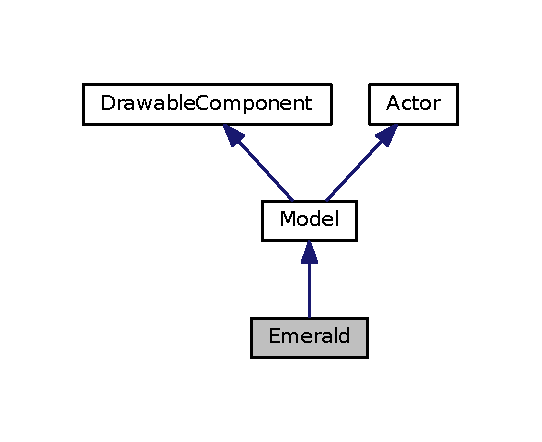
\includegraphics[width=260pt]{classEmerald__inherit__graph}
\end{center}
\end{figure}


Graphe de collaboration de Emerald\+:
\nopagebreak
\begin{figure}[H]
\begin{center}
\leavevmode
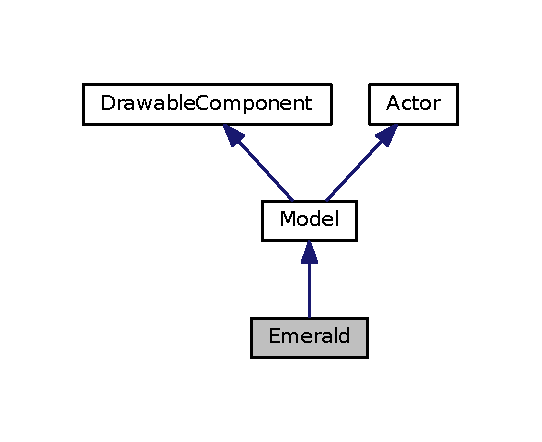
\includegraphics[width=260pt]{classEmerald__coll__graph}
\end{center}
\end{figure}


\subsection{Documentation des constructeurs et destructeur}
\hypertarget{classEmerald_a0af7339a3dfdfb13610148bb3a16c920}{\index{Emerald@{Emerald}!Emerald@{Emerald}}
\index{Emerald@{Emerald}!Emerald@{Emerald}}
\subsubsection[{Emerald}]{\setlength{\rightskip}{0pt plus 5cm}Emerald\+::\+Emerald (
\begin{DoxyParamCaption}
{}
\end{DoxyParamCaption}
)}}\label{classEmerald_a0af7339a3dfdfb13610148bb3a16c920}


Constructeur par defaut. 



Définition à la ligne 12 du fichier Emerald.\+cpp.



\subsection{Documentation des fonctions membres}
\hypertarget{classEmerald_ae913346e203ed9a8115d890bd662ea41}{\index{Emerald@{Emerald}!draw@{draw}}
\index{draw@{draw}!Emerald@{Emerald}}
\subsubsection[{draw}]{\setlength{\rightskip}{0pt plus 5cm}void Emerald\+::draw (
\begin{DoxyParamCaption}
\item[{const {\bf Camera} \&}]{cam}
\end{DoxyParamCaption}
)\hspace{0.3cm}{\ttfamily [virtual]}}}\label{classEmerald_ae913346e203ed9a8115d890bd662ea41}


Dessine une emeraude selon la camera. 


\begin{DoxyParams}{Paramètres}
{\em cam} & La camera utilisé pour le dessin \\
\hline
\end{DoxyParams}


Implémente \hyperlink{classModel_a7df7bb611f0503bc01946fff87b68fba}{Model}.



Définition à la ligne 24 du fichier Emerald.\+cpp.



Voici le graphe d'appel pour cette fonction \+:
\nopagebreak
\begin{figure}[H]
\begin{center}
\leavevmode
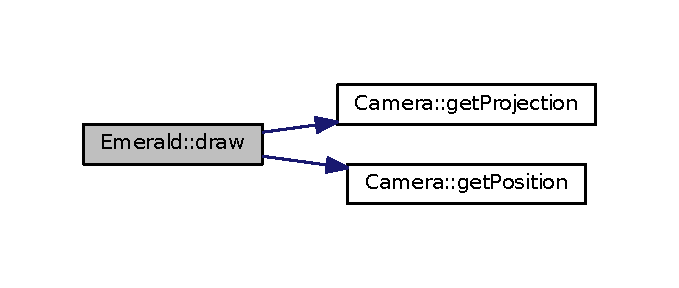
\includegraphics[width=326pt]{classEmerald_ae913346e203ed9a8115d890bd662ea41_cgraph}
\end{center}
\end{figure}


\hypertarget{classEmerald_ad997fe3bf39eb0556aefab1a91836895}{\index{Emerald@{Emerald}!update@{update}}
\index{update@{update}!Emerald@{Emerald}}
\subsubsection[{update}]{\setlength{\rightskip}{0pt plus 5cm}void Emerald\+::update (
\begin{DoxyParamCaption}
{}
\end{DoxyParamCaption}
)\hspace{0.3cm}{\ttfamily [virtual]}}}\label{classEmerald_ad997fe3bf39eb0556aefab1a91836895}


Met a jour l'etat de l'emeraude. 



Implémente \hyperlink{classModel_a4355afeacef658e098706cba1dd37118}{Model}.



Définition à la ligne 73 du fichier Emerald.\+cpp.


\hypertarget{classGLWindow}{\section{Référence de la classe G\+L\+Window}
\label{classGLWindow}\index{G\+L\+Window@{G\+L\+Window}}
}


{\ttfamily \#include $<$G\+L\+Window.\+hpp$>$}

\subsection*{Fonctions membres publiques}
\begin{DoxyCompactItemize}
\item 
\hyperlink{classGLWindow_a728e0fb2a9890114d0371c889af9f95f}{G\+L\+Window} ()
\item 
virtual \hyperlink{classGLWindow_a99612c0043db5f944500bdbd723e902b}{$\sim$\+G\+L\+Window} () final
\item 
\hyperlink{classGLWindow_a77ed0cc5ddcfa47f55b59b123cab5190}{operator G\+L\+F\+Wwindow $\ast$} () const 
\begin{DoxyCompactList}\small\item\em Permet la conversion implicite vers le type fenêtre de base. \end{DoxyCompactList}\item 
virtual int \hyperlink{classGLWindow_a297b34b4bbf69b29516e279839262623}{run} (int=0, char $\ast$$\ast$=0) override
\begin{DoxyCompactList}\small\item\em exécute la boucle de rendue \end{DoxyCompactList}\item 
std\+::shared\+\_\+ptr$<$ \hyperlink{classController}{Controller} $>$ \hyperlink{classGLWindow_a73bff0543adb7c2d3f2be1bd86306579}{get\+Controller} ()
\end{DoxyCompactItemize}
\subsection*{Fonctions membres publiques statiques}
\begin{DoxyCompactItemize}
\item 
static \hyperlink{classGLWindow}{G\+L\+Window} $\ast$ \hyperlink{classGLWindow_a00dbb194ab7a1395bc6f8e4af9d0b34a}{get\+Main\+Window} ()
\end{DoxyCompactItemize}


\subsection{Description détaillée}
La classe \hyperlink{classGLWindow}{G\+L\+Window} s'occupe de l'interface graphique et de la boucle de rendu principale 

Définition à la ligne 21 du fichier G\+L\+Window.\+hpp.



Graphe d'héritage de G\+L\+Window\+:
\nopagebreak
\begin{figure}[H]
\begin{center}
\leavevmode
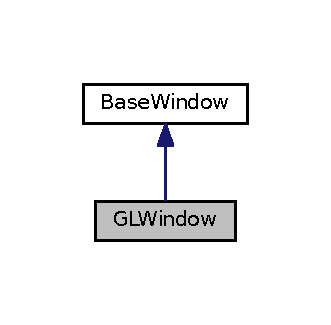
\includegraphics[width=159pt]{classGLWindow__inherit__graph}
\end{center}
\end{figure}


Graphe de collaboration de G\+L\+Window\+:
\nopagebreak
\begin{figure}[H]
\begin{center}
\leavevmode
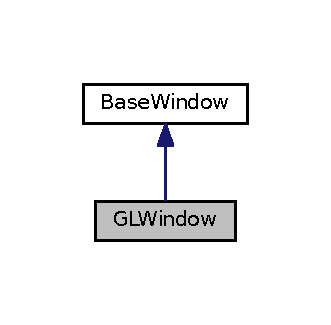
\includegraphics[width=159pt]{classGLWindow__coll__graph}
\end{center}
\end{figure}


\subsection{Documentation des constructeurs et destructeur}
\hypertarget{classGLWindow_a728e0fb2a9890114d0371c889af9f95f}{\index{G\+L\+Window@{G\+L\+Window}!G\+L\+Window@{G\+L\+Window}}
\index{G\+L\+Window@{G\+L\+Window}!G\+L\+Window@{G\+L\+Window}}
\subsubsection[{G\+L\+Window}]{\setlength{\rightskip}{0pt plus 5cm}G\+L\+Window\+::\+G\+L\+Window (
\begin{DoxyParamCaption}
{}
\end{DoxyParamCaption}
)}}\label{classGLWindow_a728e0fb2a9890114d0371c889af9f95f}


Définition à la ligne 17 du fichier G\+L\+Window.\+cpp.

\hypertarget{classGLWindow_a99612c0043db5f944500bdbd723e902b}{\index{G\+L\+Window@{G\+L\+Window}!````~G\+L\+Window@{$\sim$\+G\+L\+Window}}
\index{````~G\+L\+Window@{$\sim$\+G\+L\+Window}!G\+L\+Window@{G\+L\+Window}}
\subsubsection[{$\sim$\+G\+L\+Window}]{\setlength{\rightskip}{0pt plus 5cm}G\+L\+Window\+::$\sim$\+G\+L\+Window (
\begin{DoxyParamCaption}
{}
\end{DoxyParamCaption}
)\hspace{0.3cm}{\ttfamily [final]}, {\ttfamily [virtual]}}}\label{classGLWindow_a99612c0043db5f944500bdbd723e902b}


Définition à la ligne 102 du fichier G\+L\+Window.\+cpp.



\subsection{Documentation des fonctions membres}
\hypertarget{classGLWindow_a73bff0543adb7c2d3f2be1bd86306579}{\index{G\+L\+Window@{G\+L\+Window}!get\+Controller@{get\+Controller}}
\index{get\+Controller@{get\+Controller}!G\+L\+Window@{G\+L\+Window}}
\subsubsection[{get\+Controller}]{\setlength{\rightskip}{0pt plus 5cm}std\+::shared\+\_\+ptr$<${\bf Controller}$>$ G\+L\+Window\+::get\+Controller (
\begin{DoxyParamCaption}
{}
\end{DoxyParamCaption}
)\hspace{0.3cm}{\ttfamily [inline]}}}\label{classGLWindow_a73bff0543adb7c2d3f2be1bd86306579}
\begin{DoxyReturn}{Renvoie}
un pointeur sur l'instance existante de la manette 
\end{DoxyReturn}


Définition à la ligne 55 du fichier G\+L\+Window.\+hpp.

\hypertarget{classGLWindow_a00dbb194ab7a1395bc6f8e4af9d0b34a}{\index{G\+L\+Window@{G\+L\+Window}!get\+Main\+Window@{get\+Main\+Window}}
\index{get\+Main\+Window@{get\+Main\+Window}!G\+L\+Window@{G\+L\+Window}}
\subsubsection[{get\+Main\+Window}]{\setlength{\rightskip}{0pt plus 5cm}{\bf G\+L\+Window} $\ast$ G\+L\+Window\+::get\+Main\+Window (
\begin{DoxyParamCaption}
{}
\end{DoxyParamCaption}
)\hspace{0.3cm}{\ttfamily [static]}}}\label{classGLWindow_a00dbb194ab7a1395bc6f8e4af9d0b34a}
\begin{DoxyReturn}{Renvoie}
un pointeur sur l'instance existante de la fenêtre 
\end{DoxyReturn}


Définition à la ligne 30 du fichier G\+L\+Window.\+cpp.



Voici le graphe d'appel pour cette fonction \+:
\nopagebreak
\begin{figure}[H]
\begin{center}
\leavevmode
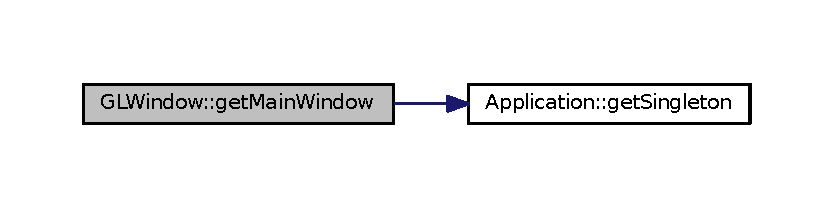
\includegraphics[width=350pt]{classGLWindow_a00dbb194ab7a1395bc6f8e4af9d0b34a_cgraph}
\end{center}
\end{figure}


\hypertarget{classGLWindow_a77ed0cc5ddcfa47f55b59b123cab5190}{\index{G\+L\+Window@{G\+L\+Window}!operator G\+L\+F\+Wwindow $\ast$@{operator G\+L\+F\+Wwindow $\ast$}}
\index{operator G\+L\+F\+Wwindow $\ast$@{operator G\+L\+F\+Wwindow $\ast$}!G\+L\+Window@{G\+L\+Window}}
\subsubsection[{operator G\+L\+F\+Wwindow $\ast$}]{\setlength{\rightskip}{0pt plus 5cm}G\+L\+Window\+::operator G\+L\+F\+Wwindow $\ast$ (
\begin{DoxyParamCaption}
{}
\end{DoxyParamCaption}
) const\hspace{0.3cm}{\ttfamily [inline]}}}\label{classGLWindow_a77ed0cc5ddcfa47f55b59b123cab5190}


Permet la conversion implicite vers le type fenêtre de base. 

\begin{DoxyReturn}{Renvoie}
un pointeur sur la fenêtre de base 
\end{DoxyReturn}


Définition à la ligne 40 du fichier G\+L\+Window.\+hpp.

\hypertarget{classGLWindow_a297b34b4bbf69b29516e279839262623}{\index{G\+L\+Window@{G\+L\+Window}!run@{run}}
\index{run@{run}!G\+L\+Window@{G\+L\+Window}}
\subsubsection[{run}]{\setlength{\rightskip}{0pt plus 5cm}int G\+L\+Window\+::run (
\begin{DoxyParamCaption}
\item[{int}]{argc = {\ttfamily 0}, }
\item[{char $\ast$$\ast$}]{argv = {\ttfamily 0}}
\end{DoxyParamCaption}
)\hspace{0.3cm}{\ttfamily [override]}, {\ttfamily [virtual]}}}\label{classGLWindow_a297b34b4bbf69b29516e279839262623}


exécute la boucle de rendue 


\begin{DoxyParams}{Paramètres}
{\em argc} & Le nombre d'arguments \\
\hline
{\em argv} & argc arguments \\
\hline
\end{DoxyParams}
\begin{DoxyReturn}{Renvoie}
l'état de sortie 
\end{DoxyReturn}


Implémente \hyperlink{classBaseWindow_a2faf52e77b0c61225d81be8b25afd661}{Base\+Window}.



Définition à la ligne 37 du fichier G\+L\+Window.\+cpp.



Voici le graphe d'appel pour cette fonction \+:
\nopagebreak
\begin{figure}[H]
\begin{center}
\leavevmode
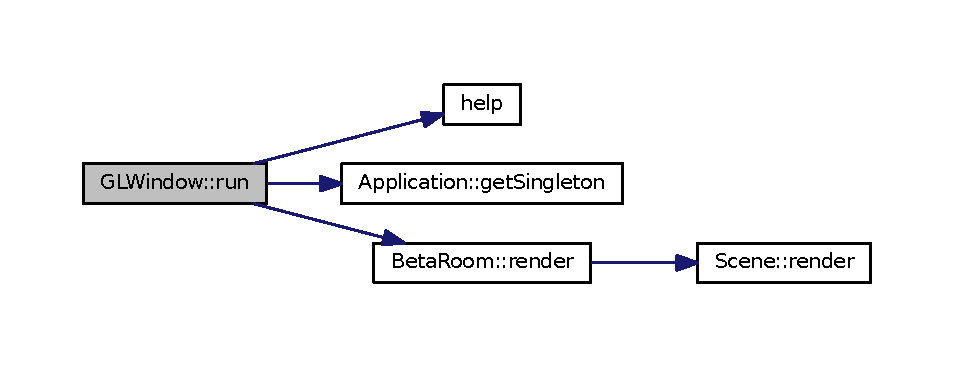
\includegraphics[width=350pt]{classGLWindow_a297b34b4bbf69b29516e279839262623_cgraph}
\end{center}
\end{figure}



\hypertarget{structLogger}{\section{Référence de la classe Logger}
\label{structLogger}\index{Logger@{Logger}}
}


{\ttfamily \#include $<$Log.\+hpp$>$}

\subsection*{Types publics}
\begin{DoxyCompactItemize}
\item 
enum \{ \\*
\hyperlink{structLogger_a737161d132f5296b6a6a387e702343aca56db48fa2adaf90cde424c8ecfb8e5e1}{Debug}, 
\hyperlink{structLogger_a737161d132f5296b6a6a387e702343acaaf07afd601e9c0e4c30c394462f99159}{Normal}, 
\hyperlink{structLogger_a737161d132f5296b6a6a387e702343aca9f3354efabc848dcb9ddf68279b7417b}{Info}, 
\hyperlink{structLogger_a737161d132f5296b6a6a387e702343aca77a6bb9c2e4acdedd73247b641a61778}{Warning}, 
\\*
\hyperlink{structLogger_a737161d132f5296b6a6a387e702343acaf38b93fc7958d816f1e769f264632e68}{Error}, 
\hyperlink{structLogger_a737161d132f5296b6a6a387e702343aca16f37b00dd31e0c3699a8079fc733930}{Critical}
 \}
\begin{DoxyCompactList}\small\item\em Cette énumeration contient les différents niveau d'urgence existant. \end{DoxyCompactList}\end{DoxyCompactItemize}
\subsection*{Fonctions membres publiques}
\begin{DoxyCompactItemize}
\item 
\hyperlink{structLogger_a3d7fbd0388f4fe493e0ba30a0ef87e7d}{Logger} (int Filter=0, int Fd=2)
\item 
void \hyperlink{structLogger_ac9e1e59987a134104efa32d419fb3a05}{operator()} (const std\+::string \&rhs=std\+::string(), int lvl=1) const 
\end{DoxyCompactItemize}
\subsection*{Champs de données}
\begin{DoxyCompactItemize}
\item 
int \hyperlink{structLogger_ad2ee79af4600bdc5f362c999f86ae718}{filter}
\item 
int \hyperlink{structLogger_aed0c1f4ae52e15c00906b158131a5775}{fd}
\end{DoxyCompactItemize}


\subsection{Description détaillée}
Gère les informations à afficher, selon le niveau parametré 

Définition à la ligne 9 du fichier Log.\+hpp.



\subsection{Documentation des énumérations membres}
\hypertarget{structLogger_a737161d132f5296b6a6a387e702343ac}{\subsubsection[{anonymous enum}]{\setlength{\rightskip}{0pt plus 5cm}anonymous enum}}\label{structLogger_a737161d132f5296b6a6a387e702343ac}


Cette énumeration contient les différents niveau d'urgence existant. 

\begin{Desc}
\item[Valeurs énumérées]\par
\begin{description}
\index{Debug@{Debug}!Logger@{Logger}}\index{Logger@{Logger}!Debug@{Debug}}\item[{\em 
\hypertarget{structLogger_a737161d132f5296b6a6a387e702343aca56db48fa2adaf90cde424c8ecfb8e5e1}{Debug}\label{structLogger_a737161d132f5296b6a6a387e702343aca56db48fa2adaf90cde424c8ecfb8e5e1}
}]\index{Normal@{Normal}!Logger@{Logger}}\index{Logger@{Logger}!Normal@{Normal}}\item[{\em 
\hypertarget{structLogger_a737161d132f5296b6a6a387e702343acaaf07afd601e9c0e4c30c394462f99159}{Normal}\label{structLogger_a737161d132f5296b6a6a387e702343acaaf07afd601e9c0e4c30c394462f99159}
}]\index{Info@{Info}!Logger@{Logger}}\index{Logger@{Logger}!Info@{Info}}\item[{\em 
\hypertarget{structLogger_a737161d132f5296b6a6a387e702343aca9f3354efabc848dcb9ddf68279b7417b}{Info}\label{structLogger_a737161d132f5296b6a6a387e702343aca9f3354efabc848dcb9ddf68279b7417b}
}]\index{Warning@{Warning}!Logger@{Logger}}\index{Logger@{Logger}!Warning@{Warning}}\item[{\em 
\hypertarget{structLogger_a737161d132f5296b6a6a387e702343aca77a6bb9c2e4acdedd73247b641a61778}{Warning}\label{structLogger_a737161d132f5296b6a6a387e702343aca77a6bb9c2e4acdedd73247b641a61778}
}]\index{Error@{Error}!Logger@{Logger}}\index{Logger@{Logger}!Error@{Error}}\item[{\em 
\hypertarget{structLogger_a737161d132f5296b6a6a387e702343acaf38b93fc7958d816f1e769f264632e68}{Error}\label{structLogger_a737161d132f5296b6a6a387e702343acaf38b93fc7958d816f1e769f264632e68}
}]\index{Critical@{Critical}!Logger@{Logger}}\index{Logger@{Logger}!Critical@{Critical}}\item[{\em 
\hypertarget{structLogger_a737161d132f5296b6a6a387e702343aca16f37b00dd31e0c3699a8079fc733930}{Critical}\label{structLogger_a737161d132f5296b6a6a387e702343aca16f37b00dd31e0c3699a8079fc733930}
}]\end{description}
\end{Desc}


Définition à la ligne 28 du fichier Log.\+hpp.



\subsection{Documentation des constructeurs et destructeur}
\hypertarget{structLogger_a3d7fbd0388f4fe493e0ba30a0ef87e7d}{\index{Logger@{Logger}!Logger@{Logger}}
\index{Logger@{Logger}!Logger@{Logger}}
\subsubsection[{Logger}]{\setlength{\rightskip}{0pt plus 5cm}Logger\+::\+Logger (
\begin{DoxyParamCaption}
\item[{int}]{Filter = {\ttfamily 0}, }
\item[{int}]{Fd = {\ttfamily 2}}
\end{DoxyParamCaption}
)\hspace{0.3cm}{\ttfamily [inline]}}}\label{structLogger_a3d7fbd0388f4fe493e0ba30a0ef87e7d}

\begin{DoxyParams}{Paramètres}
{\em Filter} & Niveau de filtre \\
\hline
{\em Fd} & Descripteur du fichier dans lequel écrire les logs. \\
\hline
\end{DoxyParams}


Définition à la ligne 25 du fichier Log.\+hpp.



\subsection{Documentation des fonctions membres}
\hypertarget{structLogger_ac9e1e59987a134104efa32d419fb3a05}{\index{Logger@{Logger}!operator()@{operator()}}
\index{operator()@{operator()}!Logger@{Logger}}
\subsubsection[{operator()}]{\setlength{\rightskip}{0pt plus 5cm}void Logger\+::operator() (
\begin{DoxyParamCaption}
\item[{const std\+::string \&}]{rhs = {\ttfamily std\+:\+:string()}, }
\item[{int}]{lvl = {\ttfamily 1}}
\end{DoxyParamCaption}
) const\hspace{0.3cm}{\ttfamily [inline]}}}\label{structLogger_ac9e1e59987a134104efa32d419fb3a05}

\begin{DoxyParams}{Paramètres}
{\em rhs} & Chaine à écrire \\
\hline
{\em lvl} & Niveau d'urgence \\
\hline
\end{DoxyParams}


Définition à la ligne 42 du fichier Log.\+hpp.



\subsection{Documentation des champs}
\hypertarget{structLogger_aed0c1f4ae52e15c00906b158131a5775}{\index{Logger@{Logger}!fd@{fd}}
\index{fd@{fd}!Logger@{Logger}}
\subsubsection[{fd}]{\setlength{\rightskip}{0pt plus 5cm}Logger\+::fd}}\label{structLogger_aed0c1f4ae52e15c00906b158131a5775}
Descripteur du fichier dans lequel écrire les logs. 

Définition à la ligne 20 du fichier Log.\+hpp.

\hypertarget{structLogger_ad2ee79af4600bdc5f362c999f86ae718}{\index{Logger@{Logger}!filter@{filter}}
\index{filter@{filter}!Logger@{Logger}}
\subsubsection[{filter}]{\setlength{\rightskip}{0pt plus 5cm}Logger\+::filter}}\label{structLogger_ad2ee79af4600bdc5f362c999f86ae718}
Niveau de sortie autorisé, les demandes de log avec un niveau inférieur à cette variable ne seront pas reportés 

Définition à la ligne 20 du fichier Log.\+hpp.


\hypertarget{classMesh}{\section{Référence de la classe Mesh}
\label{classMesh}\index{Mesh@{Mesh}}
}


{\ttfamily \#include $<$Mesh.\+hpp$>$}

\subsection*{Fonctions membres publiques}
\begin{DoxyCompactItemize}
\item 
\hyperlink{classMesh_a2af137f1571af89172b9c102302c416b}{Mesh} ()
\item 
virtual void \hyperlink{classMesh_aeb4e185f5d443690132b8e88bf5c669c}{draw} (const \hyperlink{classCamera}{Camera} \&)
\begin{DoxyCompactList}\small\item\em Dessine un objet sur la cible active. \end{DoxyCompactList}\item 
virtual void \hyperlink{classMesh_abb6110295efe8ae479659e46553c952a}{update} ()
\begin{DoxyCompactList}\small\item\em Met à jour un acteur. \end{DoxyCompactList}\end{DoxyCompactItemize}
\subsection*{Membres hérités additionnels}


\subsection{Description détaillée}
\begin{DoxyAuthor}{Auteur}
N.\+Boutemeur sert d'example pour deriver de \hyperlink{classModel}{Model} 
\end{DoxyAuthor}


Définition à la ligne 13 du fichier Mesh.\+hpp.



Graphe d'héritage de Mesh\+:
\nopagebreak
\begin{figure}[H]
\begin{center}
\leavevmode
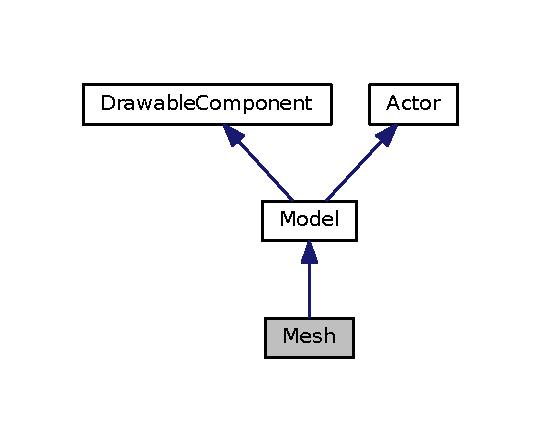
\includegraphics[width=260pt]{classMesh__inherit__graph}
\end{center}
\end{figure}


Graphe de collaboration de Mesh\+:
\nopagebreak
\begin{figure}[H]
\begin{center}
\leavevmode
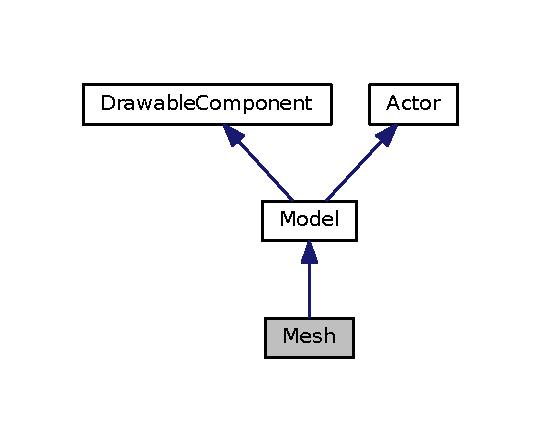
\includegraphics[width=260pt]{classMesh__coll__graph}
\end{center}
\end{figure}


\subsection{Documentation des constructeurs et destructeur}
\hypertarget{classMesh_a2af137f1571af89172b9c102302c416b}{\index{Mesh@{Mesh}!Mesh@{Mesh}}
\index{Mesh@{Mesh}!Mesh@{Mesh}}
\subsubsection[{Mesh}]{\setlength{\rightskip}{0pt plus 5cm}Mesh\+::\+Mesh (
\begin{DoxyParamCaption}
{}
\end{DoxyParamCaption}
)}}\label{classMesh_a2af137f1571af89172b9c102302c416b}


Définition à la ligne 22 du fichier Mesh.\+cpp.



\subsection{Documentation des fonctions membres}
\hypertarget{classMesh_aeb4e185f5d443690132b8e88bf5c669c}{\index{Mesh@{Mesh}!draw@{draw}}
\index{draw@{draw}!Mesh@{Mesh}}
\subsubsection[{draw}]{\setlength{\rightskip}{0pt plus 5cm}void Mesh\+::draw (
\begin{DoxyParamCaption}
\item[{const {\bf Camera} \&}]{}
\end{DoxyParamCaption}
)\hspace{0.3cm}{\ttfamily [virtual]}}}\label{classMesh_aeb4e185f5d443690132b8e88bf5c669c}


Dessine un objet sur la cible active. 



Implémente \hyperlink{classModel_a7df7bb611f0503bc01946fff87b68fba}{Model}.



Définition à la ligne 33 du fichier Mesh.\+cpp.



Voici le graphe d'appel pour cette fonction \+:
\nopagebreak
\begin{figure}[H]
\begin{center}
\leavevmode
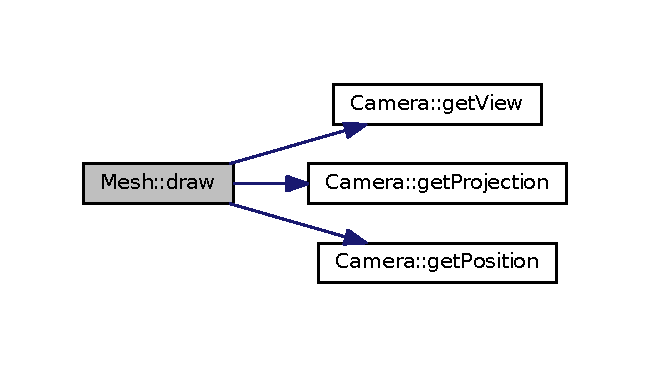
\includegraphics[width=312pt]{classMesh_aeb4e185f5d443690132b8e88bf5c669c_cgraph}
\end{center}
\end{figure}


\hypertarget{classMesh_abb6110295efe8ae479659e46553c952a}{\index{Mesh@{Mesh}!update@{update}}
\index{update@{update}!Mesh@{Mesh}}
\subsubsection[{update}]{\setlength{\rightskip}{0pt plus 5cm}virtual void Mesh\+::update (
\begin{DoxyParamCaption}
{}
\end{DoxyParamCaption}
)\hspace{0.3cm}{\ttfamily [inline]}, {\ttfamily [virtual]}}}\label{classMesh_abb6110295efe8ae479659e46553c952a}


Met à jour un acteur. 



Implémente \hyperlink{classModel_a4355afeacef658e098706cba1dd37118}{Model}.



Définition à la ligne 21 du fichier Mesh.\+hpp.


\hypertarget{classModel}{\section{Référence de la classe Model}
\label{classModel}\index{Model@{Model}}
}


{\ttfamily \#include $<$Model.\+hpp$>$}

\subsection*{Fonctions membres publiques}
\begin{DoxyCompactItemize}
\item 
virtual \hyperlink{classModel_ad6ebd2062a0b823db841a0b88baac4c0}{$\sim$\+Model} ()
\item 
virtual void \hyperlink{classModel_a7df7bb611f0503bc01946fff87b68fba}{draw} (const \hyperlink{classCamera}{Camera} \&)=0
\begin{DoxyCompactList}\small\item\em Dessine un objet sur la cible active. \end{DoxyCompactList}\item 
virtual void \hyperlink{classModel_a4355afeacef658e098706cba1dd37118}{update} ()=0
\begin{DoxyCompactList}\small\item\em Met à jour un acteur. \end{DoxyCompactList}\item 
void \hyperlink{classModel_a5714a558b8e85b9e86c91782d7ef5ba5}{set\+Scale} (const glm\+::vec3 \&)
\begin{DoxyCompactList}\small\item\em Elargi le modèle. \end{DoxyCompactList}\item 
void \hyperlink{classModel_a5ad6354ec2a10f6866485b04172a2be5}{set\+Position} (const glm\+::vec3 \&)
\begin{DoxyCompactList}\small\item\em Déplace le modèle. \end{DoxyCompactList}\item 
void \hyperlink{classModel_a41649d6e7b259cfdb362a57d14191b91}{set\+Rotation} (const glm\+::vec3 \&)
\begin{DoxyCompactList}\small\item\em Tourne le modèle sur l'axe X. \end{DoxyCompactList}\end{DoxyCompactItemize}
\subsection*{Fonctions membres protégées}
\begin{DoxyCompactItemize}
\item 
\hyperlink{classModel_a83f93ebbe04926f639fbedbf78a7c760}{Model} (const std\+::string \&)
\begin{DoxyCompactList}\small\item\em Instancie un model d'apres le code source O\+B\+J. \end{DoxyCompactList}\item 
\hyperlink{classModel_a15d7d92731e90feee6e2d68dca9cf8a1}{Model} (const float $\ast$, unsigned, const unsigned $\ast$=nullptr, unsigned=0)
\begin{DoxyCompactList}\small\item\em Instancie un modèle d'après un tableau de sommet et un tableau d'éléments. \end{DoxyCompactList}\item 
\hyperlink{classModel_a6401b781378ee497f3862139948b91d4}{Model} (const std\+::vector$<$ float $>$ \&)
\begin{DoxyCompactList}\small\item\em Instancie un modèle d'après le tableau. \end{DoxyCompactList}\item 
\hyperlink{classModel_a820453a93d6e36c9d79ef370650e0988}{Model} (const std\+::vector$<$ float $>$ \&, const std\+::vector$<$ unsigned $>$ \&)
\begin{DoxyCompactList}\small\item\em Instancie un modèle d'après le tableau et les éléments. \end{DoxyCompactList}\item 
void \hyperlink{classModel_a8b977a20040024b1f04c9badcc177391}{rebuild\+Model\+Mat} ()
\begin{DoxyCompactList}\small\item\em Met à jour la matrice de transformation. \end{DoxyCompactList}\end{DoxyCompactItemize}
\subsection*{Attributs protégés}
\begin{DoxyCompactItemize}
\item 
std\+::shared\+\_\+ptr$<$ \hyperlink{classController}{Controller} $>$ \hyperlink{classModel_aa952b1556f55b93129bef6e5de91b2b0}{m\+\_\+controller} = \hyperlink{classApplication_afa5d5ce6c9369e1ea05ee6540fe07dc2}{Application\+::get\+Singleton}()-\/$>$get\+Controller()
\item 
glm\+::vec3 \hyperlink{classModel_abc23ecdbd0ec986ed2ccd00fe20b817a}{m\+\_\+scale} = glm\+::vec3(1.\+0f)
\item 
glm\+::vec3 \hyperlink{classModel_a5cacbaf83f7abedb413670a877ca0342}{m\+\_\+rotation}
\item 
glm\+::vec3 \hyperlink{classModel_af1de9a151d77a2a7c9448fc796c2aee1}{m\+\_\+position}
\item 
unsigned \hyperlink{classModel_acba5e05b4023cae6c5650ae839fb009f}{m\+\_\+vao} = 0
\item 
unsigned \hyperlink{classModel_a76ec368b072bc97855bd860d9eaf879b}{m\+\_\+vbo} = 0
\item 
unsigned \hyperlink{classModel_a56668d2e99c519c8dbe00c3aab4f7d09}{m\+\_\+ebo} = -\/1
\item 
glm\+::mat4 \hyperlink{classModel_a415a19bd8f5afaf29a40ddc02496b15f}{m\+\_\+model\+Matrix}
\item 
int \hyperlink{classModel_a2e6cb8d2533906b5b67ff6e46979b6ba}{vert\+Num}
\item 
int \hyperlink{classModel_a6552e6870c67e02fba57b86a09859b91}{face\+Num}
\end{DoxyCompactItemize}


\subsection{Description détaillée}
\begin{DoxyAuthor}{Auteur}
N.\+Boutemeur n'est pas instanciable par elle mémé, elle doit être dérivée pour pouvoir l'utiliser 
\end{DoxyAuthor}


Définition à la ligne 22 du fichier Model.\+hpp.



Graphe d'héritage de Model\+:
\nopagebreak
\begin{figure}[H]
\begin{center}
\leavevmode
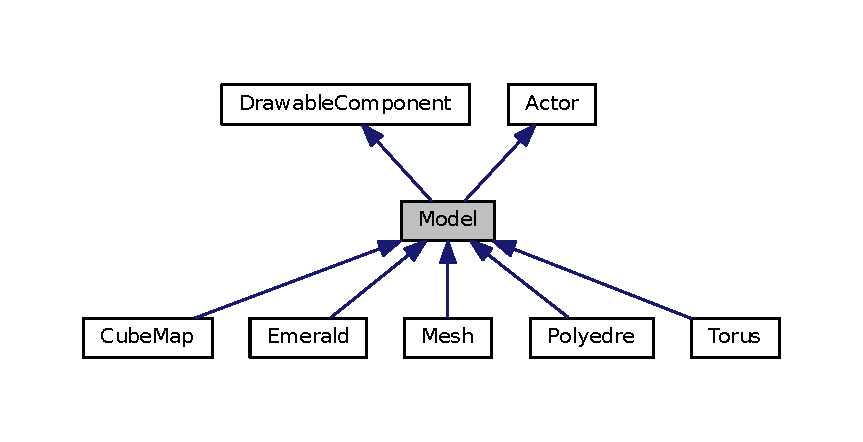
\includegraphics[width=350pt]{classModel__inherit__graph}
\end{center}
\end{figure}


Graphe de collaboration de Model\+:
\nopagebreak
\begin{figure}[H]
\begin{center}
\leavevmode
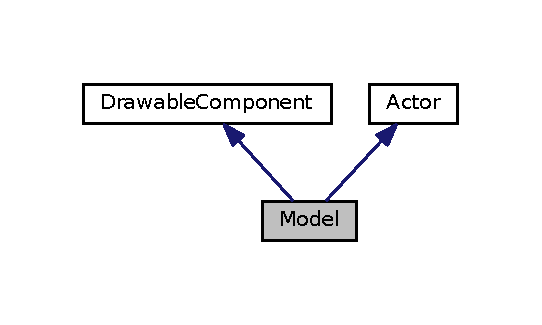
\includegraphics[width=260pt]{classModel__coll__graph}
\end{center}
\end{figure}


\subsection{Documentation des constructeurs et destructeur}
\hypertarget{classModel_ad6ebd2062a0b823db841a0b88baac4c0}{\index{Model@{Model}!````~Model@{$\sim$\+Model}}
\index{````~Model@{$\sim$\+Model}!Model@{Model}}
\subsubsection[{$\sim$\+Model}]{\setlength{\rightskip}{0pt plus 5cm}Model\+::$\sim$\+Model (
\begin{DoxyParamCaption}
{}
\end{DoxyParamCaption}
)\hspace{0.3cm}{\ttfamily [virtual]}}}\label{classModel_ad6ebd2062a0b823db841a0b88baac4c0}


Définition à la ligne 83 du fichier Model.\+cpp.

\hypertarget{classModel_a83f93ebbe04926f639fbedbf78a7c760}{\index{Model@{Model}!Model@{Model}}
\index{Model@{Model}!Model@{Model}}
\subsubsection[{Model}]{\setlength{\rightskip}{0pt plus 5cm}Model\+::\+Model (
\begin{DoxyParamCaption}
\item[{const std\+::string \&}]{O\+B\+J\+Source}
\end{DoxyParamCaption}
)\hspace{0.3cm}{\ttfamily [protected]}}}\label{classModel_a83f93ebbe04926f639fbedbf78a7c760}


Instancie un model d'apres le code source O\+B\+J. 



Définition à la ligne 13 du fichier Model.\+cpp.

\hypertarget{classModel_a15d7d92731e90feee6e2d68dca9cf8a1}{\index{Model@{Model}!Model@{Model}}
\index{Model@{Model}!Model@{Model}}
\subsubsection[{Model}]{\setlength{\rightskip}{0pt plus 5cm}Model\+::\+Model (
\begin{DoxyParamCaption}
\item[{const float $\ast$}]{v\+Data, }
\item[{unsigned}]{vsize, }
\item[{const unsigned $\ast$}]{elements = {\ttfamily nullptr}, }
\item[{unsigned}]{esize = {\ttfamily 0}}
\end{DoxyParamCaption}
)\hspace{0.3cm}{\ttfamily [protected]}}}\label{classModel_a15d7d92731e90feee6e2d68dca9cf8a1}


Instancie un modèle d'après un tableau de sommet et un tableau d'éléments. 



Définition à la ligne 50 du fichier Model.\+cpp.

\hypertarget{classModel_a6401b781378ee497f3862139948b91d4}{\index{Model@{Model}!Model@{Model}}
\index{Model@{Model}!Model@{Model}}
\subsubsection[{Model}]{\setlength{\rightskip}{0pt plus 5cm}Model\+::\+Model (
\begin{DoxyParamCaption}
\item[{const std\+::vector$<$ float $>$ \&}]{v\+Data}
\end{DoxyParamCaption}
)\hspace{0.3cm}{\ttfamily [protected]}}}\label{classModel_a6401b781378ee497f3862139948b91d4}


Instancie un modèle d'après le tableau. 



Définition à la ligne 76 du fichier Model.\+cpp.

\hypertarget{classModel_a820453a93d6e36c9d79ef370650e0988}{\index{Model@{Model}!Model@{Model}}
\index{Model@{Model}!Model@{Model}}
\subsubsection[{Model}]{\setlength{\rightskip}{0pt plus 5cm}Model\+::\+Model (
\begin{DoxyParamCaption}
\item[{const std\+::vector$<$ float $>$ \&}]{v\+Data, }
\item[{const std\+::vector$<$ unsigned $>$ \&}]{elements}
\end{DoxyParamCaption}
)\hspace{0.3cm}{\ttfamily [protected]}}}\label{classModel_a820453a93d6e36c9d79ef370650e0988}


Instancie un modèle d'après le tableau et les éléments. 



Définition à la ligne 79 du fichier Model.\+cpp.



\subsection{Documentation des fonctions membres}
\hypertarget{classModel_a7df7bb611f0503bc01946fff87b68fba}{\index{Model@{Model}!draw@{draw}}
\index{draw@{draw}!Model@{Model}}
\subsubsection[{draw}]{\setlength{\rightskip}{0pt plus 5cm}virtual void Model\+::draw (
\begin{DoxyParamCaption}
\item[{const {\bf Camera} \&}]{}
\end{DoxyParamCaption}
)\hspace{0.3cm}{\ttfamily [pure virtual]}}}\label{classModel_a7df7bb611f0503bc01946fff87b68fba}


Dessine un objet sur la cible active. 



Implémente \hyperlink{structDrawableComponent_ad1b6696a0f1ab135c9b2109450c75928}{Drawable\+Component}.



Implémenté dans \hyperlink{classEmerald_ae913346e203ed9a8115d890bd662ea41}{Emerald}, \hyperlink{classCubeMap_a9e042ac0b15cf9a28af3320b769f140f}{Cube\+Map}, \hyperlink{classPolyedre_a57ffd7e5fbba07e8b9c9737a4507a37b}{Polyedre}, \hyperlink{classTorus_a4d7971c04def3d60c37b1018560dcfb2}{Torus}, et \hyperlink{classMesh_aeb4e185f5d443690132b8e88bf5c669c}{Mesh}.

\hypertarget{classModel_a8b977a20040024b1f04c9badcc177391}{\index{Model@{Model}!rebuild\+Model\+Mat@{rebuild\+Model\+Mat}}
\index{rebuild\+Model\+Mat@{rebuild\+Model\+Mat}!Model@{Model}}
\subsubsection[{rebuild\+Model\+Mat}]{\setlength{\rightskip}{0pt plus 5cm}void Model\+::rebuild\+Model\+Mat (
\begin{DoxyParamCaption}
{}
\end{DoxyParamCaption}
)\hspace{0.3cm}{\ttfamily [protected]}}}\label{classModel_a8b977a20040024b1f04c9badcc177391}


Met à jour la matrice de transformation. 



Définition à la ligne 92 du fichier Model.\+cpp.



Voici le graphe des appelants de cette fonction \+:
\nopagebreak
\begin{figure}[H]
\begin{center}
\leavevmode
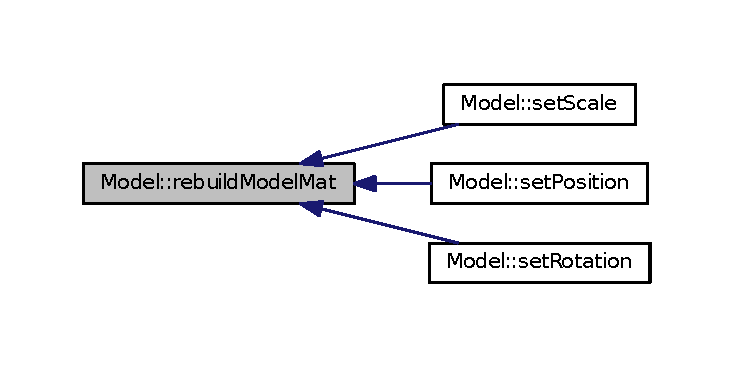
\includegraphics[width=350pt]{classModel_a8b977a20040024b1f04c9badcc177391_icgraph}
\end{center}
\end{figure}


\hypertarget{classModel_a5ad6354ec2a10f6866485b04172a2be5}{\index{Model@{Model}!set\+Position@{set\+Position}}
\index{set\+Position@{set\+Position}!Model@{Model}}
\subsubsection[{set\+Position}]{\setlength{\rightskip}{0pt plus 5cm}void Model\+::set\+Position (
\begin{DoxyParamCaption}
\item[{const glm\+::vec3 \&}]{pos}
\end{DoxyParamCaption}
)}}\label{classModel_a5ad6354ec2a10f6866485b04172a2be5}


Déplace le modèle. 



Définition à la ligne 109 du fichier Model.\+cpp.



Voici le graphe d'appel pour cette fonction \+:
\nopagebreak
\begin{figure}[H]
\begin{center}
\leavevmode
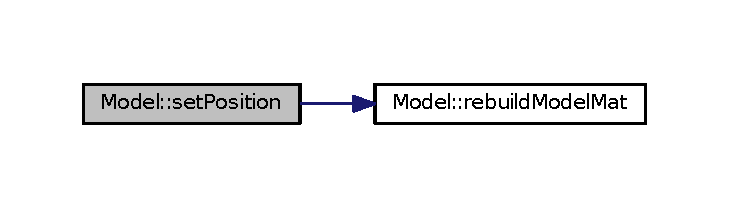
\includegraphics[width=350pt]{classModel_a5ad6354ec2a10f6866485b04172a2be5_cgraph}
\end{center}
\end{figure}


\hypertarget{classModel_a41649d6e7b259cfdb362a57d14191b91}{\index{Model@{Model}!set\+Rotation@{set\+Rotation}}
\index{set\+Rotation@{set\+Rotation}!Model@{Model}}
\subsubsection[{set\+Rotation}]{\setlength{\rightskip}{0pt plus 5cm}void Model\+::set\+Rotation (
\begin{DoxyParamCaption}
\item[{const glm\+::vec3 \&}]{rot}
\end{DoxyParamCaption}
)}}\label{classModel_a41649d6e7b259cfdb362a57d14191b91}


Tourne le modèle sur l'axe X. 



Définition à la ligne 115 du fichier Model.\+cpp.



Voici le graphe d'appel pour cette fonction \+:
\nopagebreak
\begin{figure}[H]
\begin{center}
\leavevmode
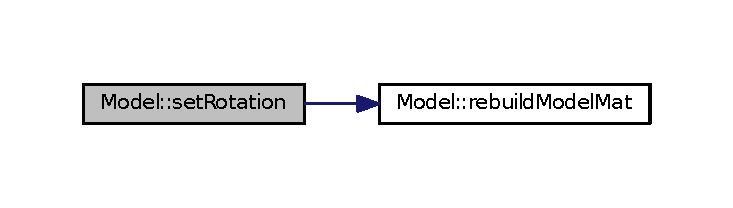
\includegraphics[width=350pt]{classModel_a41649d6e7b259cfdb362a57d14191b91_cgraph}
\end{center}
\end{figure}


\hypertarget{classModel_a5714a558b8e85b9e86c91782d7ef5ba5}{\index{Model@{Model}!set\+Scale@{set\+Scale}}
\index{set\+Scale@{set\+Scale}!Model@{Model}}
\subsubsection[{set\+Scale}]{\setlength{\rightskip}{0pt plus 5cm}void Model\+::set\+Scale (
\begin{DoxyParamCaption}
\item[{const glm\+::vec3 \&}]{scale}
\end{DoxyParamCaption}
)}}\label{classModel_a5714a558b8e85b9e86c91782d7ef5ba5}


Elargi le modèle. 



Définition à la ligne 103 du fichier Model.\+cpp.



Voici le graphe d'appel pour cette fonction \+:
\nopagebreak
\begin{figure}[H]
\begin{center}
\leavevmode
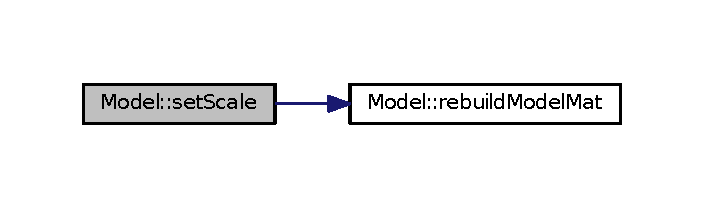
\includegraphics[width=338pt]{classModel_a5714a558b8e85b9e86c91782d7ef5ba5_cgraph}
\end{center}
\end{figure}


\hypertarget{classModel_a4355afeacef658e098706cba1dd37118}{\index{Model@{Model}!update@{update}}
\index{update@{update}!Model@{Model}}
\subsubsection[{update}]{\setlength{\rightskip}{0pt plus 5cm}virtual void Model\+::update (
\begin{DoxyParamCaption}
{}
\end{DoxyParamCaption}
)\hspace{0.3cm}{\ttfamily [pure virtual]}}}\label{classModel_a4355afeacef658e098706cba1dd37118}


Met à jour un acteur. 



Implémente \hyperlink{structActor_a4363e3b26c7903de41423a2fb1fc5f6e}{Actor}.



Implémenté dans \hyperlink{classEmerald_ad997fe3bf39eb0556aefab1a91836895}{Emerald}, \hyperlink{classCubeMap_af4766b5a5fafe3ce6e2cd8905b192d1c}{Cube\+Map}, \hyperlink{classPolyedre_a9ea5863ed9ee46c090e5dbafeda0ef73}{Polyedre}, \hyperlink{classTorus_ac63e15f0274b1beb5e8f7f968c2ac69f}{Torus}, et \hyperlink{classMesh_abb6110295efe8ae479659e46553c952a}{Mesh}.



\subsection{Documentation des champs}
\hypertarget{classModel_a6552e6870c67e02fba57b86a09859b91}{\index{Model@{Model}!face\+Num@{face\+Num}}
\index{face\+Num@{face\+Num}!Model@{Model}}
\subsubsection[{face\+Num}]{\setlength{\rightskip}{0pt plus 5cm}Model\+::face\+Num\hspace{0.3cm}{\ttfamily [protected]}}}\label{classModel_a6552e6870c67e02fba57b86a09859b91}
{\ttfamily Nombre} de faces 

Définition à la ligne 75 du fichier Model.\+hpp.

\hypertarget{classModel_aa952b1556f55b93129bef6e5de91b2b0}{\index{Model@{Model}!m\+\_\+controller@{m\+\_\+controller}}
\index{m\+\_\+controller@{m\+\_\+controller}!Model@{Model}}
\subsubsection[{m\+\_\+controller}]{\setlength{\rightskip}{0pt plus 5cm}Model\+::m\+\_\+controller = {\bf Application\+::get\+Singleton}()-\/$>$get\+Controller()\hspace{0.3cm}{\ttfamily [protected]}}}\label{classModel_aa952b1556f55b93129bef6e5de91b2b0}
Référence à l'instance existante de la manette 

Définition à la ligne 47 du fichier Model.\+hpp.

\hypertarget{classModel_a56668d2e99c519c8dbe00c3aab4f7d09}{\index{Model@{Model}!m\+\_\+ebo@{m\+\_\+ebo}}
\index{m\+\_\+ebo@{m\+\_\+ebo}!Model@{Model}}
\subsubsection[{m\+\_\+ebo}]{\setlength{\rightskip}{0pt plus 5cm}Model\+::m\+\_\+ebo = -\/1\hspace{0.3cm}{\ttfamily [protected]}}}\label{classModel_a56668d2e99c519c8dbe00c3aab4f7d09}
{\ttfamily Identifiant} du Element Buffer Object 

Définition à la ligne 61 du fichier Model.\+hpp.

\hypertarget{classModel_a415a19bd8f5afaf29a40ddc02496b15f}{\index{Model@{Model}!m\+\_\+model\+Matrix@{m\+\_\+model\+Matrix}}
\index{m\+\_\+model\+Matrix@{m\+\_\+model\+Matrix}!Model@{Model}}
\subsubsection[{m\+\_\+model\+Matrix}]{\setlength{\rightskip}{0pt plus 5cm}Model\+::m\+\_\+model\+Matrix\hspace{0.3cm}{\ttfamily [protected]}}}\label{classModel_a415a19bd8f5afaf29a40ddc02496b15f}
{\ttfamily Matrice} de model 

Définition à la ligne 66 du fichier Model.\+hpp.

\hypertarget{classModel_af1de9a151d77a2a7c9448fc796c2aee1}{\index{Model@{Model}!m\+\_\+position@{m\+\_\+position}}
\index{m\+\_\+position@{m\+\_\+position}!Model@{Model}}
\subsubsection[{m\+\_\+position}]{\setlength{\rightskip}{0pt plus 5cm}glm\+::vec3 Model\+::m\+\_\+position\hspace{0.3cm}{\ttfamily [protected]}}}\label{classModel_af1de9a151d77a2a7c9448fc796c2aee1}


Définition à la ligne 48 du fichier Model.\+hpp.

\hypertarget{classModel_a5cacbaf83f7abedb413670a877ca0342}{\index{Model@{Model}!m\+\_\+rotation@{m\+\_\+rotation}}
\index{m\+\_\+rotation@{m\+\_\+rotation}!Model@{Model}}
\subsubsection[{m\+\_\+rotation}]{\setlength{\rightskip}{0pt plus 5cm}glm\+::vec3 Model\+::m\+\_\+rotation\hspace{0.3cm}{\ttfamily [protected]}}}\label{classModel_a5cacbaf83f7abedb413670a877ca0342}


Définition à la ligne 48 du fichier Model.\+hpp.

\hypertarget{classModel_abc23ecdbd0ec986ed2ccd00fe20b817a}{\index{Model@{Model}!m\+\_\+scale@{m\+\_\+scale}}
\index{m\+\_\+scale@{m\+\_\+scale}!Model@{Model}}
\subsubsection[{m\+\_\+scale}]{\setlength{\rightskip}{0pt plus 5cm}glm\+::vec3 Model\+::m\+\_\+scale = glm\+::vec3(1.\+0f)\hspace{0.3cm}{\ttfamily [protected]}}}\label{classModel_abc23ecdbd0ec986ed2ccd00fe20b817a}


Définition à la ligne 48 du fichier Model.\+hpp.

\hypertarget{classModel_acba5e05b4023cae6c5650ae839fb009f}{\index{Model@{Model}!m\+\_\+vao@{m\+\_\+vao}}
\index{m\+\_\+vao@{m\+\_\+vao}!Model@{Model}}
\subsubsection[{m\+\_\+vao}]{\setlength{\rightskip}{0pt plus 5cm}Model\+::m\+\_\+vao = 0\hspace{0.3cm}{\ttfamily [protected]}}}\label{classModel_acba5e05b4023cae6c5650ae839fb009f}
{\ttfamily Identifiant} du \hyperlink{structVertex}{Vertex} Array Object 

Définition à la ligne 61 du fichier Model.\+hpp.

\hypertarget{classModel_a76ec368b072bc97855bd860d9eaf879b}{\index{Model@{Model}!m\+\_\+vbo@{m\+\_\+vbo}}
\index{m\+\_\+vbo@{m\+\_\+vbo}!Model@{Model}}
\subsubsection[{m\+\_\+vbo}]{\setlength{\rightskip}{0pt plus 5cm}Model\+::m\+\_\+vbo = 0\hspace{0.3cm}{\ttfamily [protected]}}}\label{classModel_a76ec368b072bc97855bd860d9eaf879b}
{\ttfamily Identifiant} du \hyperlink{structVertex}{Vertex} Buffer Object 

Définition à la ligne 61 du fichier Model.\+hpp.

\hypertarget{classModel_a2e6cb8d2533906b5b67ff6e46979b6ba}{\index{Model@{Model}!vert\+Num@{vert\+Num}}
\index{vert\+Num@{vert\+Num}!Model@{Model}}
\subsubsection[{vert\+Num}]{\setlength{\rightskip}{0pt plus 5cm}Model\+::vert\+Num\hspace{0.3cm}{\ttfamily [protected]}}}\label{classModel_a2e6cb8d2533906b5b67ff6e46979b6ba}
{\ttfamily Nombre} de sommets 

Définition à la ligne 75 du fichier Model.\+hpp.


\hypertarget{classOBJData}{\section{Référence de la classe O\+B\+J\+Data}
\label{classOBJData}\index{O\+B\+J\+Data@{O\+B\+J\+Data}}
}


{\ttfamily \#include $<$O\+B\+J\+Data.\+hpp$>$}

\subsection*{Fonctions membres publiques}
\begin{DoxyCompactItemize}
\item 
\hyperlink{classOBJData_aca7fa2cb5246604b3187e0ccfd66e838}{O\+B\+J\+Data} (const std\+::string \&obj\+File)
\begin{DoxyCompactList}\small\item\em Parcours une string et en créer une représentation interne. \end{DoxyCompactList}\item 
std\+::vector$<$ float $>$ \hyperlink{classOBJData_ae34192969b5459608871fb9068282e2a}{get\+Data} ()
\begin{DoxyCompactList}\small\item\em Construit un tableau prêt à l'emploi. \end{DoxyCompactList}\end{DoxyCompactItemize}


\subsection{Description détaillée}
représente les données présente dans un fichier O\+B\+J 

Définition à la ligne 74 du fichier O\+B\+J\+Data.\+hpp.



\subsection{Documentation des constructeurs et destructeur}
\hypertarget{classOBJData_aca7fa2cb5246604b3187e0ccfd66e838}{\index{O\+B\+J\+Data@{O\+B\+J\+Data}!O\+B\+J\+Data@{O\+B\+J\+Data}}
\index{O\+B\+J\+Data@{O\+B\+J\+Data}!O\+B\+J\+Data@{O\+B\+J\+Data}}
\subsubsection[{O\+B\+J\+Data}]{\setlength{\rightskip}{0pt plus 5cm}O\+B\+J\+Data\+::\+O\+B\+J\+Data (
\begin{DoxyParamCaption}
\item[{const std\+::string \&}]{obj\+File}
\end{DoxyParamCaption}
)}}\label{classOBJData_aca7fa2cb5246604b3187e0ccfd66e838}


Parcours une string et en créer une représentation interne. 


\begin{DoxyParams}{Paramètres}
{\em obj\+File} & Code source du fichier O\+B\+J \\
\hline
\end{DoxyParams}


Définition à la ligne 87 du fichier O\+B\+J\+Data.\+cpp.



Voici le graphe d'appel pour cette fonction \+:
\nopagebreak
\begin{figure}[H]
\begin{center}
\leavevmode
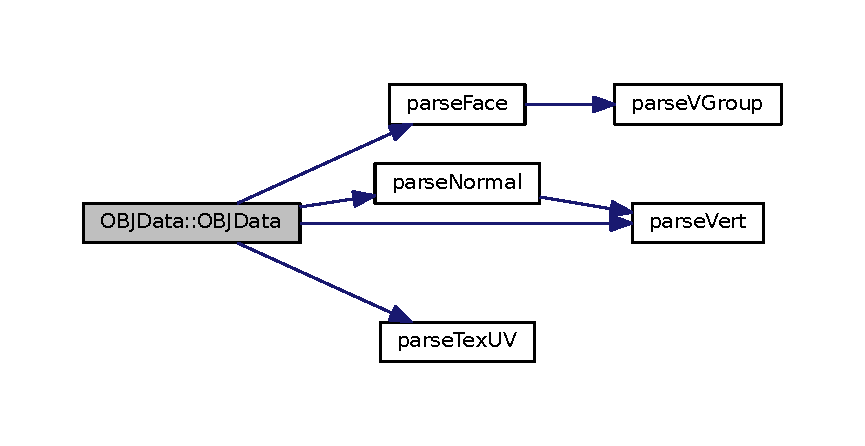
\includegraphics[width=350pt]{classOBJData_aca7fa2cb5246604b3187e0ccfd66e838_cgraph}
\end{center}
\end{figure}




\subsection{Documentation des fonctions membres}
\hypertarget{classOBJData_ae34192969b5459608871fb9068282e2a}{\index{O\+B\+J\+Data@{O\+B\+J\+Data}!get\+Data@{get\+Data}}
\index{get\+Data@{get\+Data}!O\+B\+J\+Data@{O\+B\+J\+Data}}
\subsubsection[{get\+Data}]{\setlength{\rightskip}{0pt plus 5cm}vector$<$ float $>$ O\+B\+J\+Data\+::get\+Data (
\begin{DoxyParamCaption}
{}
\end{DoxyParamCaption}
)}}\label{classOBJData_ae34192969b5459608871fb9068282e2a}


Construit un tableau prêt à l'emploi. 

\begin{DoxyReturn}{Renvoie}
Un tableau de float constitué de n points de 8 floats chacun sous la forme \mbox{[}xyz uv abc\mbox{]} 
\end{DoxyReturn}


Définition à la ligne 138 du fichier O\+B\+J\+Data.\+cpp.


\hypertarget{classPolyedre}{\section{Référence de la classe Polyedre}
\label{classPolyedre}\index{Polyedre@{Polyedre}}
}


{\ttfamily \#include $<$Polyedre.\+hpp$>$}

\subsection*{Fonctions membres publiques}
\begin{DoxyCompactItemize}
\item 
\hyperlink{classPolyedre_a03cdf6d5bd3c00c62d9e174eafe92699}{Polyedre} ()
\item 
virtual void \hyperlink{classPolyedre_a57ffd7e5fbba07e8b9c9737a4507a37b}{draw} (const \hyperlink{classCamera}{Camera} \&)
\begin{DoxyCompactList}\small\item\em Dessine un objet sur la cible active. \end{DoxyCompactList}\item 
virtual void \hyperlink{classPolyedre_a9ea5863ed9ee46c090e5dbafeda0ef73}{update} ()
\begin{DoxyCompactList}\small\item\em Met à jour un acteur. \end{DoxyCompactList}\end{DoxyCompactItemize}
\subsection*{Membres hérités additionnels}


\subsection{Description détaillée}
\begin{DoxyAuthor}{Auteur}
N.\+Boutemeur
\end{DoxyAuthor}
La classe \hyperlink{classPolyedre}{Polyedre} defini un cristal qui est dessinable 

Définition à la ligne 15 du fichier Polyedre.\+hpp.



Graphe d'héritage de Polyedre\+:
\nopagebreak
\begin{figure}[H]
\begin{center}
\leavevmode
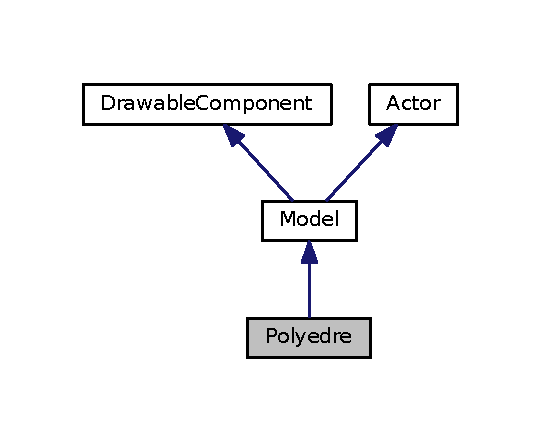
\includegraphics[width=260pt]{classPolyedre__inherit__graph}
\end{center}
\end{figure}


Graphe de collaboration de Polyedre\+:
\nopagebreak
\begin{figure}[H]
\begin{center}
\leavevmode
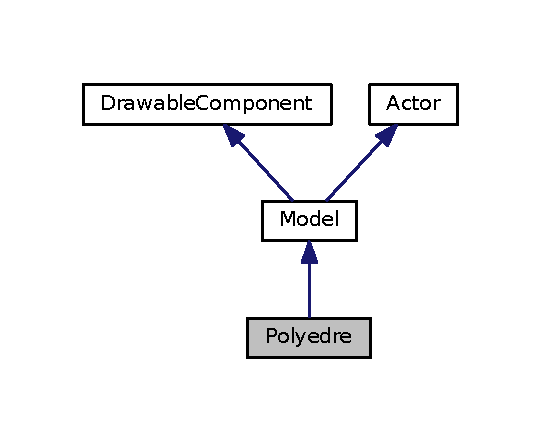
\includegraphics[width=260pt]{classPolyedre__coll__graph}
\end{center}
\end{figure}


\subsection{Documentation des constructeurs et destructeur}
\hypertarget{classPolyedre_a03cdf6d5bd3c00c62d9e174eafe92699}{\index{Polyedre@{Polyedre}!Polyedre@{Polyedre}}
\index{Polyedre@{Polyedre}!Polyedre@{Polyedre}}
\subsubsection[{Polyedre}]{\setlength{\rightskip}{0pt plus 5cm}Polyedre\+::\+Polyedre (
\begin{DoxyParamCaption}
{}
\end{DoxyParamCaption}
)}}\label{classPolyedre_a03cdf6d5bd3c00c62d9e174eafe92699}


Définition à la ligne 14 du fichier Polyedre.\+cpp.



\subsection{Documentation des fonctions membres}
\hypertarget{classPolyedre_a57ffd7e5fbba07e8b9c9737a4507a37b}{\index{Polyedre@{Polyedre}!draw@{draw}}
\index{draw@{draw}!Polyedre@{Polyedre}}
\subsubsection[{draw}]{\setlength{\rightskip}{0pt plus 5cm}void Polyedre\+::draw (
\begin{DoxyParamCaption}
\item[{const {\bf Camera} \&}]{}
\end{DoxyParamCaption}
)\hspace{0.3cm}{\ttfamily [virtual]}}}\label{classPolyedre_a57ffd7e5fbba07e8b9c9737a4507a37b}


Dessine un objet sur la cible active. 



Implémente \hyperlink{classModel_a7df7bb611f0503bc01946fff87b68fba}{Model}.



Définition à la ligne 26 du fichier Polyedre.\+cpp.



Voici le graphe d'appel pour cette fonction \+:
\nopagebreak
\begin{figure}[H]
\begin{center}
\leavevmode
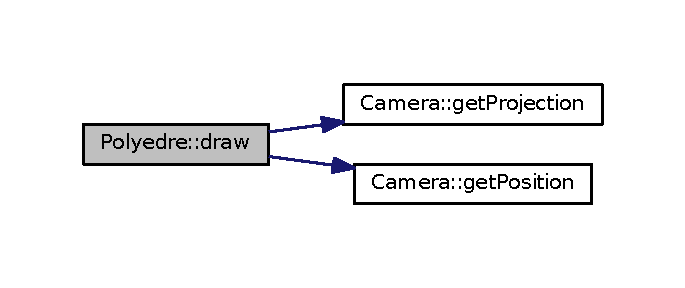
\includegraphics[width=329pt]{classPolyedre_a57ffd7e5fbba07e8b9c9737a4507a37b_cgraph}
\end{center}
\end{figure}


\hypertarget{classPolyedre_a9ea5863ed9ee46c090e5dbafeda0ef73}{\index{Polyedre@{Polyedre}!update@{update}}
\index{update@{update}!Polyedre@{Polyedre}}
\subsubsection[{update}]{\setlength{\rightskip}{0pt plus 5cm}void Polyedre\+::update (
\begin{DoxyParamCaption}
{}
\end{DoxyParamCaption}
)\hspace{0.3cm}{\ttfamily [virtual]}}}\label{classPolyedre_a9ea5863ed9ee46c090e5dbafeda0ef73}


Met à jour un acteur. 



Implémente \hyperlink{classModel_a4355afeacef658e098706cba1dd37118}{Model}.



Définition à la ligne 66 du fichier Polyedre.\+cpp.


\hypertarget{classResourceManager}{\section{Référence de la classe Resource\+Manager}
\label{classResourceManager}\index{Resource\+Manager@{Resource\+Manager}}
}


{\ttfamily \#include $<$Resource\+Manager.\+hpp$>$}

\subsection*{Fonctions membres publiques}
\begin{DoxyCompactItemize}
\item 
void \hyperlink{classResourceManager_aa812c98a716dfa62c2bc3f71b4e20e98}{add\+File} (const std\+::string \&)
\begin{DoxyCompactList}\small\item\em Ajoute un fichier à l'archive. Si le fichier est une archive, alors son contenu est ajouté \end{DoxyCompactList}\item 
void \hyperlink{classResourceManager_a10f59a5ddf5a7dbdd203240386630797}{add\+Data} (const std\+::string \&, const std\+::vector$<$ unsigned char $>$ \&)
\begin{DoxyCompactList}\small\item\em Ajoute des données à l'archive. \end{DoxyCompactList}\item 
void \hyperlink{classResourceManager_ac534a350e6fbba1ef293e86aaed47bc2}{save\+Resource} (const std\+::string \&File)
\begin{DoxyCompactList}\small\item\em Sauvegarde l'archive dans un fichier. \end{DoxyCompactList}\item 
void \hyperlink{classResourceManager_aa5879e275263e1dc3750cac2005e314e}{save\+Resource} (int)
\begin{DoxyCompactList}\small\item\em Écrit l'archive dans un descripteur de fichier. \end{DoxyCompactList}\item 
std\+::vector$<$ unsigned char $>$ \hyperlink{classResourceManager_aba892a2f43fd3cfe0a757b8477ea7ca3}{get\+Data} (const std\+::string \&Handle)
\begin{DoxyCompactList}\small\item\em Récupère les données d'une ressource de l'archive. \end{DoxyCompactList}\item 
std\+::string \hyperlink{classResourceManager_ae642fd96b5cf5e2a6ee19db107b9ae03}{get\+String} (const std\+::string \&Handle)
\begin{DoxyCompactList}\small\item\em Récupère les données d'une ressource sous la forme d'une chaîne. \end{DoxyCompactList}\item 
std\+::map$<$ std\+::string, \hyperlink{ResourceManager_8hpp_ac29d54814dbcb83b635aface304200ae}{Resource} $>$ \hyperlink{classResourceManager_aff0d8b5b68006034bd31d67e6aaea3fb}{get\+Ressources} ()
\begin{DoxyCompactList}\small\item\em Renvois toute les ressources de l'archive. \end{DoxyCompactList}\end{DoxyCompactItemize}
\subsection*{Fonctions membres publiques statiques}
\begin{DoxyCompactItemize}
\item 
static std\+::shared\+\_\+ptr\\*
$<$ \hyperlink{classResourceManager}{Resource\+Manager} $>$ \hyperlink{classResourceManager_a832206535b73564824f1102b5ed5844f}{from\+Data} (const std\+::vector$<$ unsigned char $>$ \&data)
\begin{DoxyCompactList}\small\item\em Instancie un gestionnaire à partir de données. \end{DoxyCompactList}\item 
static std\+::shared\+\_\+ptr\\*
$<$ \hyperlink{classResourceManager}{Resource\+Manager} $>$ \hyperlink{classResourceManager_a90b982650eab524ba9b45942732147d9}{from\+File} (const std\+::string \&File)
\begin{DoxyCompactList}\small\item\em Instancie un gestionnaire à partir d'un fichier. \end{DoxyCompactList}\end{DoxyCompactItemize}


\subsection{Description détaillée}


Définition à la ligne 13 du fichier Resource\+Manager.\+hpp.



Graphe d'héritage de Resource\+Manager\+:
\nopagebreak
\begin{figure}[H]
\begin{center}
\leavevmode
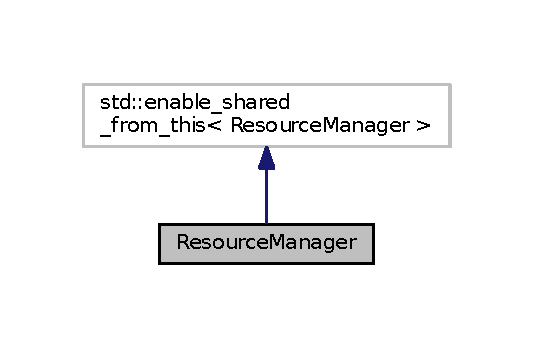
\includegraphics[width=256pt]{classResourceManager__inherit__graph}
\end{center}
\end{figure}


Graphe de collaboration de Resource\+Manager\+:
\nopagebreak
\begin{figure}[H]
\begin{center}
\leavevmode
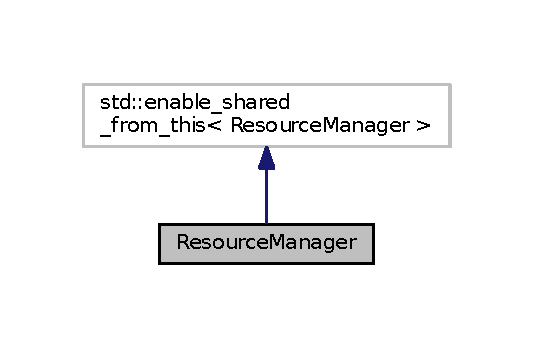
\includegraphics[width=256pt]{classResourceManager__coll__graph}
\end{center}
\end{figure}


\subsection{Documentation des fonctions membres}
\hypertarget{classResourceManager_a10f59a5ddf5a7dbdd203240386630797}{\index{Resource\+Manager@{Resource\+Manager}!add\+Data@{add\+Data}}
\index{add\+Data@{add\+Data}!Resource\+Manager@{Resource\+Manager}}
\subsubsection[{add\+Data}]{\setlength{\rightskip}{0pt plus 5cm}void Resource\+Manager\+::add\+Data (
\begin{DoxyParamCaption}
\item[{const std\+::string \&}]{Handle, }
\item[{const std\+::vector$<$ unsigned char $>$ \&}]{data}
\end{DoxyParamCaption}
)}}\label{classResourceManager_a10f59a5ddf5a7dbdd203240386630797}


Ajoute des données à l'archive. 


\begin{DoxyParams}{Paramètres}
{\em Handle} & Le nom à donner à la ressource \\
\hline
{\em data} & Les données à ajouter \\
\hline
\end{DoxyParams}


Définition à la ligne 88 du fichier Resource\+Manager.\+cpp.



Voici le graphe des appelants de cette fonction \+:
\nopagebreak
\begin{figure}[H]
\begin{center}
\leavevmode
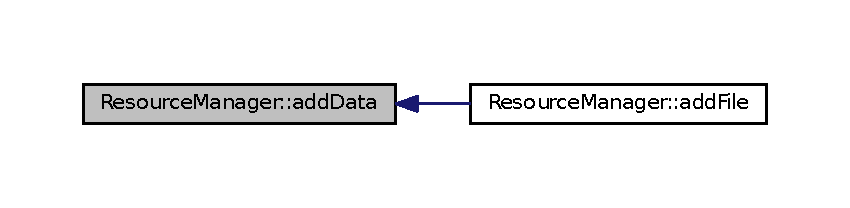
\includegraphics[width=350pt]{classResourceManager_a10f59a5ddf5a7dbdd203240386630797_icgraph}
\end{center}
\end{figure}


\hypertarget{classResourceManager_aa812c98a716dfa62c2bc3f71b4e20e98}{\index{Resource\+Manager@{Resource\+Manager}!add\+File@{add\+File}}
\index{add\+File@{add\+File}!Resource\+Manager@{Resource\+Manager}}
\subsubsection[{add\+File}]{\setlength{\rightskip}{0pt plus 5cm}void Resource\+Manager\+::add\+File (
\begin{DoxyParamCaption}
\item[{const std\+::string \&}]{File}
\end{DoxyParamCaption}
)}}\label{classResourceManager_aa812c98a716dfa62c2bc3f71b4e20e98}


Ajoute un fichier à l'archive. Si le fichier est une archive, alors son contenu est ajouté 


\begin{DoxyParams}{Paramètres}
{\em File} & fichier à ajouter \\
\hline
\end{DoxyParams}


Définition à la ligne 72 du fichier Resource\+Manager.\+cpp.



Voici le graphe d'appel pour cette fonction \+:
\nopagebreak
\begin{figure}[H]
\begin{center}
\leavevmode
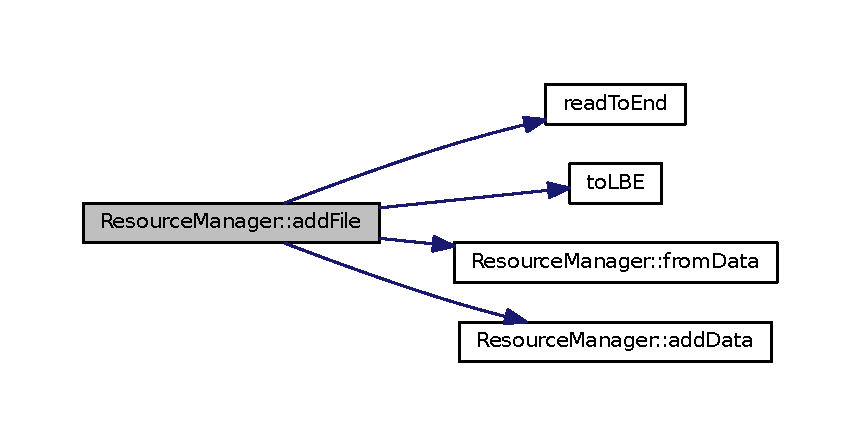
\includegraphics[width=350pt]{classResourceManager_aa812c98a716dfa62c2bc3f71b4e20e98_cgraph}
\end{center}
\end{figure}


\hypertarget{classResourceManager_a832206535b73564824f1102b5ed5844f}{\index{Resource\+Manager@{Resource\+Manager}!from\+Data@{from\+Data}}
\index{from\+Data@{from\+Data}!Resource\+Manager@{Resource\+Manager}}
\subsubsection[{from\+Data}]{\setlength{\rightskip}{0pt plus 5cm}shared\+\_\+ptr$<$ {\bf Resource\+Manager} $>$ Resource\+Manager\+::from\+Data (
\begin{DoxyParamCaption}
\item[{const std\+::vector$<$ unsigned char $>$ \&}]{data}
\end{DoxyParamCaption}
)\hspace{0.3cm}{\ttfamily [static]}}}\label{classResourceManager_a832206535b73564824f1102b5ed5844f}


Instancie un gestionnaire à partir de données. 


\begin{DoxyParams}{Paramètres}
{\em data} & Les données à lire \\
\hline
\end{DoxyParams}
\begin{DoxyReturn}{Renvoie}
Un pointeur vers le gestionnaire de resources 
\end{DoxyReturn}


Définition à la ligne 99 du fichier Resource\+Manager.\+cpp.



Voici le graphe des appelants de cette fonction \+:
\nopagebreak
\begin{figure}[H]
\begin{center}
\leavevmode
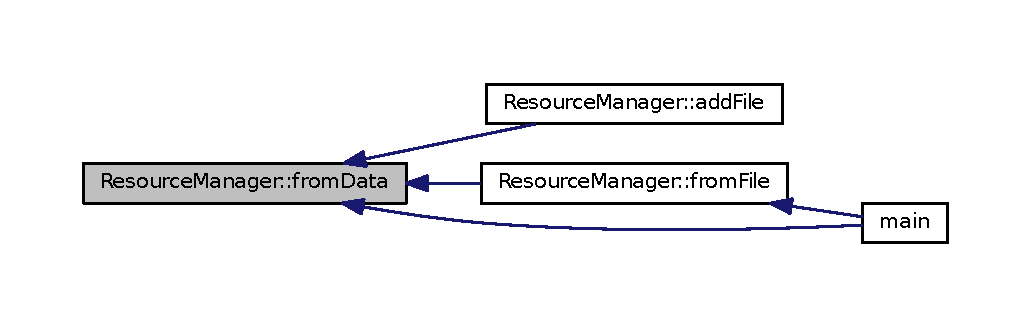
\includegraphics[width=350pt]{classResourceManager_a832206535b73564824f1102b5ed5844f_icgraph}
\end{center}
\end{figure}


\hypertarget{classResourceManager_a90b982650eab524ba9b45942732147d9}{\index{Resource\+Manager@{Resource\+Manager}!from\+File@{from\+File}}
\index{from\+File@{from\+File}!Resource\+Manager@{Resource\+Manager}}
\subsubsection[{from\+File}]{\setlength{\rightskip}{0pt plus 5cm}shared\+\_\+ptr$<$ {\bf Resource\+Manager} $>$ Resource\+Manager\+::from\+File (
\begin{DoxyParamCaption}
\item[{const std\+::string \&}]{File}
\end{DoxyParamCaption}
)\hspace{0.3cm}{\ttfamily [static]}}}\label{classResourceManager_a90b982650eab524ba9b45942732147d9}


Instancie un gestionnaire à partir d'un fichier. 


\begin{DoxyParams}{Paramètres}
{\em File} & Le fichier à lire \\
\hline
\end{DoxyParams}
\begin{DoxyReturn}{Renvoie}
Un pointeur vers le gestionnaire de resources 
\end{DoxyReturn}


Définition à la ligne 93 du fichier Resource\+Manager.\+cpp.



Voici le graphe d'appel pour cette fonction \+:
\nopagebreak
\begin{figure}[H]
\begin{center}
\leavevmode
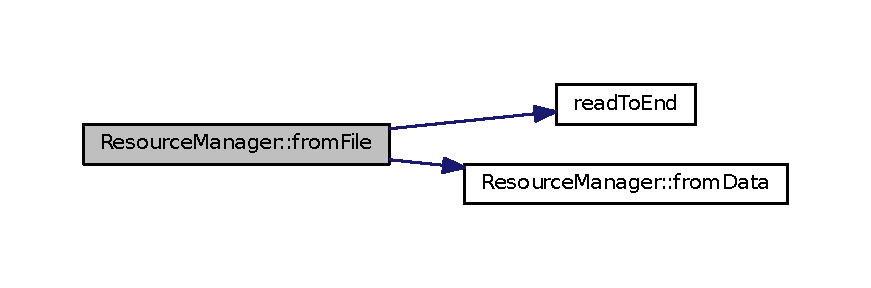
\includegraphics[width=350pt]{classResourceManager_a90b982650eab524ba9b45942732147d9_cgraph}
\end{center}
\end{figure}




Voici le graphe des appelants de cette fonction \+:
\nopagebreak
\begin{figure}[H]
\begin{center}
\leavevmode
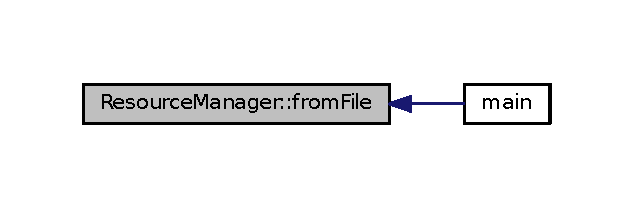
\includegraphics[width=304pt]{classResourceManager_a90b982650eab524ba9b45942732147d9_icgraph}
\end{center}
\end{figure}


\hypertarget{classResourceManager_aba892a2f43fd3cfe0a757b8477ea7ca3}{\index{Resource\+Manager@{Resource\+Manager}!get\+Data@{get\+Data}}
\index{get\+Data@{get\+Data}!Resource\+Manager@{Resource\+Manager}}
\subsubsection[{get\+Data}]{\setlength{\rightskip}{0pt plus 5cm}vector$<$ unsigned char $>$ Resource\+Manager\+::get\+Data (
\begin{DoxyParamCaption}
\item[{const std\+::string \&}]{Handle}
\end{DoxyParamCaption}
)}}\label{classResourceManager_aba892a2f43fd3cfe0a757b8477ea7ca3}


Récupère les données d'une ressource de l'archive. 


\begin{DoxyParams}{Paramètres}
{\em Handle} & Le nom de la ressource à récupérer \\
\hline
\end{DoxyParams}
\begin{DoxyReturn}{Renvoie}
Les données de la ressource 
\end{DoxyReturn}


Définition à la ligne 174 du fichier Resource\+Manager.\+cpp.

\hypertarget{classResourceManager_aff0d8b5b68006034bd31d67e6aaea3fb}{\index{Resource\+Manager@{Resource\+Manager}!get\+Ressources@{get\+Ressources}}
\index{get\+Ressources@{get\+Ressources}!Resource\+Manager@{Resource\+Manager}}
\subsubsection[{get\+Ressources}]{\setlength{\rightskip}{0pt plus 5cm}std\+::map$<$std\+::string, {\bf Resource}$>$ Resource\+Manager\+::get\+Ressources (
\begin{DoxyParamCaption}
{}
\end{DoxyParamCaption}
)}}\label{classResourceManager_aff0d8b5b68006034bd31d67e6aaea3fb}


Renvois toute les ressources de l'archive. 

\begin{DoxyReturn}{Renvoie}
Renvois toute les ressources de l'archive 
\end{DoxyReturn}
\hypertarget{classResourceManager_ae642fd96b5cf5e2a6ee19db107b9ae03}{\index{Resource\+Manager@{Resource\+Manager}!get\+String@{get\+String}}
\index{get\+String@{get\+String}!Resource\+Manager@{Resource\+Manager}}
\subsubsection[{get\+String}]{\setlength{\rightskip}{0pt plus 5cm}string Resource\+Manager\+::get\+String (
\begin{DoxyParamCaption}
\item[{const std\+::string \&}]{Handle}
\end{DoxyParamCaption}
)}}\label{classResourceManager_ae642fd96b5cf5e2a6ee19db107b9ae03}


Récupère les données d'une ressource sous la forme d'une chaîne. 


\begin{DoxyParams}{Paramètres}
{\em Handle} & Nom de la ressource \\
\hline
\end{DoxyParams}
\begin{DoxyReturn}{Renvoie}
Les données sous forme de chaîne 
\end{DoxyReturn}


Définition à la ligne 169 du fichier Resource\+Manager.\+cpp.

\hypertarget{classResourceManager_ac534a350e6fbba1ef293e86aaed47bc2}{\index{Resource\+Manager@{Resource\+Manager}!save\+Resource@{save\+Resource}}
\index{save\+Resource@{save\+Resource}!Resource\+Manager@{Resource\+Manager}}
\subsubsection[{save\+Resource}]{\setlength{\rightskip}{0pt plus 5cm}void Resource\+Manager\+::save\+Resource (
\begin{DoxyParamCaption}
\item[{const std\+::string \&}]{File}
\end{DoxyParamCaption}
)}}\label{classResourceManager_ac534a350e6fbba1ef293e86aaed47bc2}


Sauvegarde l'archive dans un fichier. 


\begin{DoxyParams}{Paramètres}
{\em File} & Nom du fichier dans lequel sauvegarder \\
\hline
\end{DoxyParams}


Définition à la ligne 104 du fichier Resource\+Manager.\+cpp.

\hypertarget{classResourceManager_aa5879e275263e1dc3750cac2005e314e}{\index{Resource\+Manager@{Resource\+Manager}!save\+Resource@{save\+Resource}}
\index{save\+Resource@{save\+Resource}!Resource\+Manager@{Resource\+Manager}}
\subsubsection[{save\+Resource}]{\setlength{\rightskip}{0pt plus 5cm}void Resource\+Manager\+::save\+Resource (
\begin{DoxyParamCaption}
\item[{int}]{fd}
\end{DoxyParamCaption}
)}}\label{classResourceManager_aa5879e275263e1dc3750cac2005e314e}


Écrit l'archive dans un descripteur de fichier. 


\begin{DoxyParams}{Paramètres}
{\em fd} & Descripteur de fichier dans lequel écrire l'archive \\
\hline
\end{DoxyParams}


Définition à la ligne 113 du fichier Resource\+Manager.\+cpp.



Voici le graphe d'appel pour cette fonction \+:
\nopagebreak
\begin{figure}[H]
\begin{center}
\leavevmode
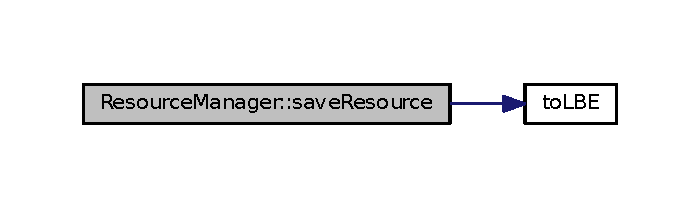
\includegraphics[width=336pt]{classResourceManager_aa5879e275263e1dc3750cac2005e314e_cgraph}
\end{center}
\end{figure}



\hypertarget{classScene}{\section{Référence de la classe Scene}
\label{classScene}\index{Scene@{Scene}}
}


{\ttfamily \#include $<$Scene.\+hpp$>$}

\subsection*{Fonctions membres publiques}
\begin{DoxyCompactItemize}
\item 
virtual void \hyperlink{classScene_a4ddf2d16f371ee9533b3faf1dd5ddfb1}{render} ()
\begin{DoxyCompactList}\small\item\em Dessine la scène sur la cible active. \end{DoxyCompactList}\item 
std\+::set$<$ std\+::shared\+\_\+ptr\\*
$<$ \hyperlink{classModel}{Model} $>$ $>$ \hyperlink{classScene_ad45e9836644de1d4c89a7a250654a409}{get\+Models} ()
\item 
virtual \hyperlink{classScene_aa0a5be58e2ee2d1fdafc5fb46b5e661e}{$\sim$\+Scene} ()
\end{DoxyCompactItemize}
\subsection*{Fonctions membres protégées}
\begin{DoxyCompactItemize}
\item 
void \hyperlink{classScene_ac4808547bb8fffe4c5a141b6f5fb663d}{add\+Model} (const std\+::shared\+\_\+ptr$<$ \hyperlink{classModel}{Model} $>$ \&model)
\begin{DoxyCompactList}\small\item\em Ajoute un modèle pour le dessin. \end{DoxyCompactList}\item 
void \hyperlink{classScene_a3b4074c80a9e1b88dbad8649c7254c2e}{add\+Effect} (const std\+::shared\+\_\+ptr$<$ \hyperlink{classEffect}{Effect} $>$ \&effect)
\begin{DoxyCompactList}\small\item\em Ajoute un modèle pour le dessin. \end{DoxyCompactList}\item 
{\footnotesize template$<$typename T $>$ }\\void \hyperlink{classScene_a3172e9ea37b589bb8641d3d42cfdd639}{add\+Model} (const T \&derived)
\begin{DoxyCompactList}\small\item\em Ajoute un modèle derivé pour le dessin. \end{DoxyCompactList}\item 
\hyperlink{classScene_ad10176d75a9cc0da56626f682d083507}{Scene} ()
\begin{DoxyCompactList}\small\item\em Construit une scène à partir d'une caméra à utiliser pour le rendu. \end{DoxyCompactList}\item 
void \hyperlink{classScene_ae0041c969f0aef8e0dd4dadfc4d3a82f}{set\+Environment} (std\+::shared\+\_\+ptr$<$ \hyperlink{classCubeMap}{Cube\+Map} $>$ env)
\end{DoxyCompactItemize}
\subsection*{Attributs protégés}
\begin{DoxyCompactItemize}
\item 
std\+::shared\+\_\+ptr$<$ \hyperlink{classCamera}{Camera} $>$ \hyperlink{classScene_ac8ac592b03402f99a2890df2603ae459}{m\+\_\+cam}
\item 
std\+::shared\+\_\+ptr$<$ \hyperlink{classCubeMap}{Cube\+Map} $>$ \hyperlink{classScene_a8424193126f3a58c21a5fe4281ed9231}{m\+\_\+cubemap}
\end{DoxyCompactItemize}


\subsection{Description détaillée}
Une scène est un ensemble d'objets destinés à être rendu, cette classe n'est pas instanciable par elle même, et doit être dérivée 

Définition à la ligne 20 du fichier Scene.\+hpp.



Graphe d'héritage de Scene\+:
\nopagebreak
\begin{figure}[H]
\begin{center}
\leavevmode
\includegraphics[width=147pt]{classScene__inherit__graph}
\end{center}
\end{figure}


\subsection{Documentation des constructeurs et destructeur}
\hypertarget{classScene_ad10176d75a9cc0da56626f682d083507}{\index{Scene@{Scene}!Scene@{Scene}}
\index{Scene@{Scene}!Scene@{Scene}}
\subsubsection[{Scene}]{\setlength{\rightskip}{0pt plus 5cm}Scene\+::\+Scene (
\begin{DoxyParamCaption}
{}
\end{DoxyParamCaption}
)\hspace{0.3cm}{\ttfamily [protected]}}}\label{classScene_ad10176d75a9cc0da56626f682d083507}


Construit une scène à partir d'une caméra à utiliser pour le rendu. 



Définition à la ligne 10 du fichier Scene.\+cpp.

\hypertarget{classScene_aa0a5be58e2ee2d1fdafc5fb46b5e661e}{\index{Scene@{Scene}!````~Scene@{$\sim$\+Scene}}
\index{````~Scene@{$\sim$\+Scene}!Scene@{Scene}}
\subsubsection[{$\sim$\+Scene}]{\setlength{\rightskip}{0pt plus 5cm}virtual Scene\+::$\sim$\+Scene (
\begin{DoxyParamCaption}
{}
\end{DoxyParamCaption}
)\hspace{0.3cm}{\ttfamily [inline]}, {\ttfamily [virtual]}}}\label{classScene_aa0a5be58e2ee2d1fdafc5fb46b5e661e}


Définition à la ligne 76 du fichier Scene.\+hpp.



\subsection{Documentation des fonctions membres}
\hypertarget{classScene_a3b4074c80a9e1b88dbad8649c7254c2e}{\index{Scene@{Scene}!add\+Effect@{add\+Effect}}
\index{add\+Effect@{add\+Effect}!Scene@{Scene}}
\subsubsection[{add\+Effect}]{\setlength{\rightskip}{0pt plus 5cm}void Scene\+::add\+Effect (
\begin{DoxyParamCaption}
\item[{const std\+::shared\+\_\+ptr$<$ {\bf Effect} $>$ \&}]{effect}
\end{DoxyParamCaption}
)\hspace{0.3cm}{\ttfamily [inline]}, {\ttfamily [protected]}}}\label{classScene_a3b4074c80a9e1b88dbad8649c7254c2e}


Ajoute un modèle pour le dessin. 



Définition à la ligne 46 du fichier Scene.\+hpp.

\hypertarget{classScene_ac4808547bb8fffe4c5a141b6f5fb663d}{\index{Scene@{Scene}!add\+Model@{add\+Model}}
\index{add\+Model@{add\+Model}!Scene@{Scene}}
\subsubsection[{add\+Model}]{\setlength{\rightskip}{0pt plus 5cm}void Scene\+::add\+Model (
\begin{DoxyParamCaption}
\item[{const std\+::shared\+\_\+ptr$<$ {\bf Model} $>$ \&}]{model}
\end{DoxyParamCaption}
)\hspace{0.3cm}{\ttfamily [inline]}, {\ttfamily [protected]}}}\label{classScene_ac4808547bb8fffe4c5a141b6f5fb663d}


Ajoute un modèle pour le dessin. 



Définition à la ligne 41 du fichier Scene.\+hpp.



Voici le graphe des appelants de cette fonction \+:
\nopagebreak
\begin{figure}[H]
\begin{center}
\leavevmode
\includegraphics[width=312pt]{classScene_ac4808547bb8fffe4c5a141b6f5fb663d_icgraph}
\end{center}
\end{figure}


\hypertarget{classScene_a3172e9ea37b589bb8641d3d42cfdd639}{\index{Scene@{Scene}!add\+Model@{add\+Model}}
\index{add\+Model@{add\+Model}!Scene@{Scene}}
\subsubsection[{add\+Model}]{\setlength{\rightskip}{0pt plus 5cm}template$<$typename T $>$ void Scene\+::add\+Model (
\begin{DoxyParamCaption}
\item[{const T \&}]{derived}
\end{DoxyParamCaption}
)\hspace{0.3cm}{\ttfamily [inline]}, {\ttfamily [protected]}}}\label{classScene_a3172e9ea37b589bb8641d3d42cfdd639}


Ajoute un modèle derivé pour le dessin. 



Définition à la ligne 52 du fichier Scene.\+hpp.



Voici le graphe d'appel pour cette fonction \+:
\nopagebreak
\begin{figure}[H]
\begin{center}
\leavevmode
\includegraphics[width=312pt]{classScene_a3172e9ea37b589bb8641d3d42cfdd639_cgraph}
\end{center}
\end{figure}


\hypertarget{classScene_ad45e9836644de1d4c89a7a250654a409}{\index{Scene@{Scene}!get\+Models@{get\+Models}}
\index{get\+Models@{get\+Models}!Scene@{Scene}}
\subsubsection[{get\+Models}]{\setlength{\rightskip}{0pt plus 5cm}std\+::set$<$std\+::shared\+\_\+ptr$<${\bf Model}$>$ $>$ Scene\+::get\+Models (
\begin{DoxyParamCaption}
{}
\end{DoxyParamCaption}
)\hspace{0.3cm}{\ttfamily [inline]}}}\label{classScene_ad45e9836644de1d4c89a7a250654a409}
\begin{DoxyReturn}{Renvoie}
Les modèles de la scène 
\end{DoxyReturn}


Définition à la ligne 75 du fichier Scene.\+hpp.

\hypertarget{classScene_a4ddf2d16f371ee9533b3faf1dd5ddfb1}{\index{Scene@{Scene}!render@{render}}
\index{render@{render}!Scene@{Scene}}
\subsubsection[{render}]{\setlength{\rightskip}{0pt plus 5cm}void Scene\+::render (
\begin{DoxyParamCaption}
{}
\end{DoxyParamCaption}
)\hspace{0.3cm}{\ttfamily [virtual]}}}\label{classScene_a4ddf2d16f371ee9533b3faf1dd5ddfb1}


Dessine la scène sur la cible active. 



Réimplémentée dans \hyperlink{classBetaRoom_a5ca4002697c35ee24a59d9d2ccab3e49}{Beta\+Room}.



Définition à la ligne 14 du fichier Scene.\+cpp.



Voici le graphe des appelants de cette fonction \+:
\nopagebreak
\begin{figure}[H]
\begin{center}
\leavevmode
\includegraphics[width=350pt]{classScene_a4ddf2d16f371ee9533b3faf1dd5ddfb1_icgraph}
\end{center}
\end{figure}


\hypertarget{classScene_ae0041c969f0aef8e0dd4dadfc4d3a82f}{\index{Scene@{Scene}!set\+Environment@{set\+Environment}}
\index{set\+Environment@{set\+Environment}!Scene@{Scene}}
\subsubsection[{set\+Environment}]{\setlength{\rightskip}{0pt plus 5cm}void Scene\+::set\+Environment (
\begin{DoxyParamCaption}
\item[{std\+::shared\+\_\+ptr$<$ {\bf Cube\+Map} $>$}]{env}
\end{DoxyParamCaption}
)\hspace{0.3cm}{\ttfamily [inline]}, {\ttfamily [protected]}}}\label{classScene_ae0041c969f0aef8e0dd4dadfc4d3a82f}


Définition à la ligne 66 du fichier Scene.\+hpp.



\subsection{Documentation des champs}
\hypertarget{classScene_ac8ac592b03402f99a2890df2603ae459}{\index{Scene@{Scene}!m\+\_\+cam@{m\+\_\+cam}}
\index{m\+\_\+cam@{m\+\_\+cam}!Scene@{Scene}}
\subsubsection[{m\+\_\+cam}]{\setlength{\rightskip}{0pt plus 5cm}Scene\+::m\+\_\+cam\hspace{0.3cm}{\ttfamily [protected]}}}\label{classScene_ac8ac592b03402f99a2890df2603ae459}
{\ttfamily Caméra} utilisée lors du rendu 

Définition à la ligne 37 du fichier Scene.\+hpp.

\hypertarget{classScene_a8424193126f3a58c21a5fe4281ed9231}{\index{Scene@{Scene}!m\+\_\+cubemap@{m\+\_\+cubemap}}
\index{m\+\_\+cubemap@{m\+\_\+cubemap}!Scene@{Scene}}
\subsubsection[{m\+\_\+cubemap}]{\setlength{\rightskip}{0pt plus 5cm}Scene\+::m\+\_\+cubemap\hspace{0.3cm}{\ttfamily [protected]}}}\label{classScene_a8424193126f3a58c21a5fe4281ed9231}
{\ttfamily la} skybox de la scene 

Définition à la ligne 65 du fichier Scene.\+hpp.


\hypertarget{classShader}{\section{Référence de la classe Shader}
\label{classShader}\index{Shader@{Shader}}
}


{\ttfamily \#include $<$Shader.\+hpp$>$}

\subsection*{Fonctions membres publiques}
\begin{DoxyCompactItemize}
\item 
\hyperlink{classShader_afafdbb306a177ca17d3ef81c30baacd3}{Shader} (const char $\ast$, const char $\ast$, const char $\ast$=nullptr)
\begin{DoxyCompactList}\small\item\em Initialise un shader. \end{DoxyCompactList}\item 
\hyperlink{classShader_aff01df87e8a102f270b5b135a295e59d}{$\sim$\+Shader} ()
\item 
int \hyperlink{classShader_a5aefd32ef08fd4da700b0bb2b75aeaf9}{get\+Programid} ()
\begin{DoxyCompactList}\small\item\em Renvois un identifiant du shader. \end{DoxyCompactList}\end{DoxyCompactItemize}
\subsection*{Fonctions membres publiques statiques}
\begin{DoxyCompactItemize}
\item 
static std\+::shared\+\_\+ptr$<$ \hyperlink{classShader}{Shader} $>$ \hyperlink{classShader_a4271c98d9ced209f007acde7a99496d1}{Basic\+Shader} ()
\begin{DoxyCompactList}\small\item\em Renvois un shader basique. \end{DoxyCompactList}\end{DoxyCompactItemize}


\subsection{Description détaillée}
\begin{DoxyAuthor}{Auteur}
N.\+Boutemeur
\end{DoxyAuthor}
La classe \hyperlink{classShader}{Shader} compile, link et gere les shaders 

Définition à la ligne 15 du fichier Shader.\+hpp.



\subsection{Documentation des constructeurs et destructeur}
\hypertarget{classShader_afafdbb306a177ca17d3ef81c30baacd3}{\index{Shader@{Shader}!Shader@{Shader}}
\index{Shader@{Shader}!Shader@{Shader}}
\subsubsection[{Shader}]{\setlength{\rightskip}{0pt plus 5cm}Shader\+::\+Shader (
\begin{DoxyParamCaption}
\item[{const char $\ast$}]{vs, }
\item[{const char $\ast$}]{ps, }
\item[{const char $\ast$}]{gs = {\ttfamily nullptr}}
\end{DoxyParamCaption}
)}}\label{classShader_afafdbb306a177ca17d3ef81c30baacd3}


Initialise un shader. 


\begin{DoxyParams}{Paramètres}
{\em vs} & Code du vertex shader \\
\hline
{\em ps} & Code du fragment shader \\
\hline
{\em gs} & Code du geometry shader \\
\hline
\end{DoxyParams}


Définition à la ligne 17 du fichier Shader.\+cpp.

\hypertarget{classShader_aff01df87e8a102f270b5b135a295e59d}{\index{Shader@{Shader}!````~Shader@{$\sim$\+Shader}}
\index{````~Shader@{$\sim$\+Shader}!Shader@{Shader}}
\subsubsection[{$\sim$\+Shader}]{\setlength{\rightskip}{0pt plus 5cm}Shader\+::$\sim$\+Shader (
\begin{DoxyParamCaption}
{}
\end{DoxyParamCaption}
)}}\label{classShader_aff01df87e8a102f270b5b135a295e59d}


Définition à la ligne 95 du fichier Shader.\+cpp.



\subsection{Documentation des fonctions membres}
\hypertarget{classShader_a4271c98d9ced209f007acde7a99496d1}{\index{Shader@{Shader}!Basic\+Shader@{Basic\+Shader}}
\index{Basic\+Shader@{Basic\+Shader}!Shader@{Shader}}
\subsubsection[{Basic\+Shader}]{\setlength{\rightskip}{0pt plus 5cm}shared\+\_\+ptr$<$ {\bf Shader} $>$ Shader\+::\+Basic\+Shader (
\begin{DoxyParamCaption}
{}
\end{DoxyParamCaption}
)\hspace{0.3cm}{\ttfamily [static]}}}\label{classShader_a4271c98d9ced209f007acde7a99496d1}


Renvois un shader basique. 

\begin{DoxyReturn}{Renvoie}
un shader basique 
\end{DoxyReturn}


Définition à la ligne 107 du fichier Shader.\+cpp.

\hypertarget{classShader_a5aefd32ef08fd4da700b0bb2b75aeaf9}{\index{Shader@{Shader}!get\+Programid@{get\+Programid}}
\index{get\+Programid@{get\+Programid}!Shader@{Shader}}
\subsubsection[{get\+Programid}]{\setlength{\rightskip}{0pt plus 5cm}int Shader\+::get\+Programid (
\begin{DoxyParamCaption}
{}
\end{DoxyParamCaption}
)\hspace{0.3cm}{\ttfamily [inline]}}}\label{classShader_a5aefd32ef08fd4da700b0bb2b75aeaf9}


Renvois un identifiant du shader. 

\begin{DoxyReturn}{Renvoie}
un identifiant du programme 
\end{DoxyReturn}


Définition à la ligne 55 du fichier Shader.\+hpp.


\hypertarget{structTextureCoordinate}{\section{Référence de la structure Texture\+Coordinate}
\label{structTextureCoordinate}\index{Texture\+Coordinate@{Texture\+Coordinate}}
}


{\ttfamily \#include $<$O\+B\+J\+Data.\+hpp$>$}

\subsection*{Champs de données}
\begin{DoxyCompactItemize}
\item 
float \hyperlink{structTextureCoordinate_a7ae310180120a5fc2aafaae29a85c68e}{u}
\begin{DoxyCompactList}\small\item\em Coordonnée U du point. \end{DoxyCompactList}\item 
float \hyperlink{structTextureCoordinate_a894c1bf1a27da48a276e5fe7bba6e200}{v}
\begin{DoxyCompactList}\small\item\em Coordonnée V du point. \end{DoxyCompactList}\end{DoxyCompactItemize}


\subsection{Description détaillée}
Représente une coordonnée de texture 

Définition à la ligne 42 du fichier O\+B\+J\+Data.\+hpp.



\subsection{Documentation des champs}
\hypertarget{structTextureCoordinate_a7ae310180120a5fc2aafaae29a85c68e}{\index{Texture\+Coordinate@{Texture\+Coordinate}!u@{u}}
\index{u@{u}!Texture\+Coordinate@{Texture\+Coordinate}}
\subsubsection[{u}]{\setlength{\rightskip}{0pt plus 5cm}Texture\+Coordinate\+::u}}\label{structTextureCoordinate_a7ae310180120a5fc2aafaae29a85c68e}


Coordonnée U du point. 



Définition à la ligne 52 du fichier O\+B\+J\+Data.\+hpp.

\hypertarget{structTextureCoordinate_a894c1bf1a27da48a276e5fe7bba6e200}{\index{Texture\+Coordinate@{Texture\+Coordinate}!v@{v}}
\index{v@{v}!Texture\+Coordinate@{Texture\+Coordinate}}
\subsubsection[{v}]{\setlength{\rightskip}{0pt plus 5cm}Texture\+Coordinate\+::v}}\label{structTextureCoordinate_a894c1bf1a27da48a276e5fe7bba6e200}


Coordonnée V du point. 



Définition à la ligne 52 du fichier O\+B\+J\+Data.\+hpp.


\hypertarget{classTorus}{\section{Référence de la classe Torus}
\label{classTorus}\index{Torus@{Torus}}
}


{\ttfamily \#include $<$Torus.\+hpp$>$}

\subsection*{Fonctions membres publiques}
\begin{DoxyCompactItemize}
\item 
\hyperlink{classTorus_ac1767993341e35d3a38676727a80047e}{Torus} ()
\item 
virtual void \hyperlink{classTorus_a4d7971c04def3d60c37b1018560dcfb2}{draw} (const \hyperlink{classCamera}{Camera} \&)
\begin{DoxyCompactList}\small\item\em Dessine un objet sur la cible active. \end{DoxyCompactList}\item 
virtual void \hyperlink{classTorus_ac63e15f0274b1beb5e8f7f968c2ac69f}{update} ()
\begin{DoxyCompactList}\small\item\em Met à jour un acteur. \end{DoxyCompactList}\end{DoxyCompactItemize}
\subsection*{Membres hérités additionnels}


\subsection{Description détaillée}


Définition à la ligne 12 du fichier Torus.\+hpp.



Graphe d'héritage de Torus\+:
\nopagebreak
\begin{figure}[H]
\begin{center}
\leavevmode
\includegraphics[width=260pt]{classTorus__inherit__graph}
\end{center}
\end{figure}


Graphe de collaboration de Torus\+:
\nopagebreak
\begin{figure}[H]
\begin{center}
\leavevmode
\includegraphics[width=260pt]{classTorus__coll__graph}
\end{center}
\end{figure}


\subsection{Documentation des constructeurs et destructeur}
\hypertarget{classTorus_ac1767993341e35d3a38676727a80047e}{\index{Torus@{Torus}!Torus@{Torus}}
\index{Torus@{Torus}!Torus@{Torus}}
\subsubsection[{Torus}]{\setlength{\rightskip}{0pt plus 5cm}Torus\+::\+Torus (
\begin{DoxyParamCaption}
{}
\end{DoxyParamCaption}
)}}\label{classTorus_ac1767993341e35d3a38676727a80047e}


Définition à la ligne 12 du fichier Torus.\+cpp.



\subsection{Documentation des fonctions membres}
\hypertarget{classTorus_a4d7971c04def3d60c37b1018560dcfb2}{\index{Torus@{Torus}!draw@{draw}}
\index{draw@{draw}!Torus@{Torus}}
\subsubsection[{draw}]{\setlength{\rightskip}{0pt plus 5cm}void Torus\+::draw (
\begin{DoxyParamCaption}
\item[{const {\bf Camera} \&}]{}
\end{DoxyParamCaption}
)\hspace{0.3cm}{\ttfamily [virtual]}}}\label{classTorus_a4d7971c04def3d60c37b1018560dcfb2}


Dessine un objet sur la cible active. 



Implémente \hyperlink{classModel_a7df7bb611f0503bc01946fff87b68fba}{Model}.



Définition à la ligne 25 du fichier Torus.\+cpp.



Voici le graphe d'appel pour cette fonction \+:
\nopagebreak
\begin{figure}[H]
\begin{center}
\leavevmode
\includegraphics[width=312pt]{classTorus_a4d7971c04def3d60c37b1018560dcfb2_cgraph}
\end{center}
\end{figure}


\hypertarget{classTorus_ac63e15f0274b1beb5e8f7f968c2ac69f}{\index{Torus@{Torus}!update@{update}}
\index{update@{update}!Torus@{Torus}}
\subsubsection[{update}]{\setlength{\rightskip}{0pt plus 5cm}void Torus\+::update (
\begin{DoxyParamCaption}
{}
\end{DoxyParamCaption}
)\hspace{0.3cm}{\ttfamily [virtual]}}}\label{classTorus_ac63e15f0274b1beb5e8f7f968c2ac69f}


Met à jour un acteur. 



Implémente \hyperlink{classModel_a4355afeacef658e098706cba1dd37118}{Model}.



Définition à la ligne 61 du fichier Torus.\+cpp.


\hypertarget{structVertex}{\section{Référence de la structure Vertex}
\label{structVertex}\index{Vertex@{Vertex}}
}


{\ttfamily \#include $<$O\+B\+J\+Data.\+hpp$>$}

\subsection*{Champs de données}
\begin{DoxyCompactItemize}
\item 
float \hyperlink{structVertex_aa19a9dc9bd9e7f4cc93053bd082c9d68}{x}
\begin{DoxyCompactList}\small\item\em Coordonnée X du point. \end{DoxyCompactList}\item 
float \hyperlink{structVertex_a094de867ef3e32b21c234cd1ebe42d61}{y}
\begin{DoxyCompactList}\small\item\em Coordonnée Y du point. \end{DoxyCompactList}\item 
float \hyperlink{structVertex_aada56d7a3ea4da97fc44b07b9cdf49b0}{z}
\begin{DoxyCompactList}\small\item\em Coordonnée Z du point. \end{DoxyCompactList}\end{DoxyCompactItemize}


\subsection{Description détaillée}
\begin{DoxyAuthor}{Auteur}
N.\+Boutemeur
\end{DoxyAuthor}
Représente une coordonnée dans l'espace 

Définition à la ligne 15 du fichier O\+B\+J\+Data.\+hpp.



\subsection{Documentation des champs}
\hypertarget{structVertex_aa19a9dc9bd9e7f4cc93053bd082c9d68}{\index{Vertex@{Vertex}!x@{x}}
\index{x@{x}!Vertex@{Vertex}}
\subsubsection[{x}]{\setlength{\rightskip}{0pt plus 5cm}Vertex\+::x}}\label{structVertex_aa19a9dc9bd9e7f4cc93053bd082c9d68}


Coordonnée X du point. 



Définition à la ligne 29 du fichier O\+B\+J\+Data.\+hpp.

\hypertarget{structVertex_a094de867ef3e32b21c234cd1ebe42d61}{\index{Vertex@{Vertex}!y@{y}}
\index{y@{y}!Vertex@{Vertex}}
\subsubsection[{y}]{\setlength{\rightskip}{0pt plus 5cm}Vertex\+::y}}\label{structVertex_a094de867ef3e32b21c234cd1ebe42d61}


Coordonnée Y du point. 



Définition à la ligne 29 du fichier O\+B\+J\+Data.\+hpp.

\hypertarget{structVertex_aada56d7a3ea4da97fc44b07b9cdf49b0}{\index{Vertex@{Vertex}!z@{z}}
\index{z@{z}!Vertex@{Vertex}}
\subsubsection[{z}]{\setlength{\rightskip}{0pt plus 5cm}Vertex\+::z}}\label{structVertex_aada56d7a3ea4da97fc44b07b9cdf49b0}


Coordonnée Z du point. 



Définition à la ligne 29 du fichier O\+B\+J\+Data.\+hpp.


\hypertarget{classXBoxController}{\section{Référence de la classe X\+Box\+Controller}
\label{classXBoxController}\index{X\+Box\+Controller@{X\+Box\+Controller}}
}


{\ttfamily \#include $<$X\+Box\+Controller.\+hpp$>$}

\subsection*{Fonctions membres publiques}
\begin{DoxyCompactItemize}
\item 
\hyperlink{classXBoxController_aebd5a50eac92047b21ce4f614c5da14d}{X\+Box\+Controller} (int, float)
\item 
virtual glm\+::vec2 \hyperlink{classXBoxController_adec21f77b6380856458c5e991c2d2805}{get\+Main\+Stick\+Position} () finaloverride
\item 
virtual glm\+::vec2 \hyperlink{classXBoxController_a6fe09f7fe9cc8439a909cbf45cdcaafd}{get\+Secondary\+Stick\+Position} () finaloverride
\item 
virtual glm\+::vec2 \hyperlink{classXBoxController_a3b3cf6e2302e80423f5ffe060cf502db}{get\+Triggers} () finaloverride
\item 
virtual std\+::vector$<$ bool $>$ \hyperlink{classXBoxController_a7f2177c57462c0f488986affcd7e8811}{get\+Buttons} () finaloverride
\item 
virtual \hyperlink{classXBoxController_a89464cf2fb5a1e3ffb03c933de70c154}{$\sim$\+X\+Box\+Controller} () finaloverride
\end{DoxyCompactItemize}


\subsection{Description détaillée}
\begin{DoxyAuthor}{Auteur}
N.\+Boutemeur
\end{DoxyAuthor}
La classe \hyperlink{classXBoxController}{X\+Box\+Controller} gère les manettes de Xbox360 connectées 

Définition à la ligne 13 du fichier X\+Box\+Controller.\+hpp.



Graphe d'héritage de X\+Box\+Controller\+:
\nopagebreak
\begin{figure}[H]
\begin{center}
\leavevmode
\includegraphics[width=169pt]{classXBoxController__inherit__graph}
\end{center}
\end{figure}


Graphe de collaboration de X\+Box\+Controller\+:
\nopagebreak
\begin{figure}[H]
\begin{center}
\leavevmode
\includegraphics[width=169pt]{classXBoxController__coll__graph}
\end{center}
\end{figure}


\subsection{Documentation des constructeurs et destructeur}
\hypertarget{classXBoxController_aebd5a50eac92047b21ce4f614c5da14d}{\index{X\+Box\+Controller@{X\+Box\+Controller}!X\+Box\+Controller@{X\+Box\+Controller}}
\index{X\+Box\+Controller@{X\+Box\+Controller}!X\+Box\+Controller@{X\+Box\+Controller}}
\subsubsection[{X\+Box\+Controller}]{\setlength{\rightskip}{0pt plus 5cm}X\+Box\+Controller\+::\+X\+Box\+Controller (
\begin{DoxyParamCaption}
\item[{int}]{joy\+Num, }
\item[{float}]{sensitivity}
\end{DoxyParamCaption}
)}}\label{classXBoxController_aebd5a50eac92047b21ce4f614c5da14d}


Définition à la ligne 31 du fichier X\+Box\+Controller.\+cpp.

\hypertarget{classXBoxController_a89464cf2fb5a1e3ffb03c933de70c154}{\index{X\+Box\+Controller@{X\+Box\+Controller}!````~X\+Box\+Controller@{$\sim$\+X\+Box\+Controller}}
\index{````~X\+Box\+Controller@{$\sim$\+X\+Box\+Controller}!X\+Box\+Controller@{X\+Box\+Controller}}
\subsubsection[{$\sim$\+X\+Box\+Controller}]{\setlength{\rightskip}{0pt plus 5cm}virtual X\+Box\+Controller\+::$\sim$\+X\+Box\+Controller (
\begin{DoxyParamCaption}
{}
\end{DoxyParamCaption}
)\hspace{0.3cm}{\ttfamily [inline]}, {\ttfamily [final]}, {\ttfamily [override]}, {\ttfamily [virtual]}}}\label{classXBoxController_a89464cf2fb5a1e3ffb03c933de70c154}


Définition à la ligne 38 du fichier X\+Box\+Controller.\+hpp.



\subsection{Documentation des fonctions membres}
\hypertarget{classXBoxController_a7f2177c57462c0f488986affcd7e8811}{\index{X\+Box\+Controller@{X\+Box\+Controller}!get\+Buttons@{get\+Buttons}}
\index{get\+Buttons@{get\+Buttons}!X\+Box\+Controller@{X\+Box\+Controller}}
\subsubsection[{get\+Buttons}]{\setlength{\rightskip}{0pt plus 5cm}vector$<$ bool $>$ X\+Box\+Controller\+::get\+Buttons (
\begin{DoxyParamCaption}
{}
\end{DoxyParamCaption}
)\hspace{0.3cm}{\ttfamily [final]}, {\ttfamily [override]}, {\ttfamily [virtual]}}}\label{classXBoxController_a7f2177c57462c0f488986affcd7e8811}
\begin{DoxyReturn}{Renvoie}
Les boutons pressés 
\end{DoxyReturn}


Implémente \hyperlink{classController_af7483fe863ff38bd2e9617771c450931}{Controller}.



Définition à la ligne 71 du fichier X\+Box\+Controller.\+cpp.

\hypertarget{classXBoxController_adec21f77b6380856458c5e991c2d2805}{\index{X\+Box\+Controller@{X\+Box\+Controller}!get\+Main\+Stick\+Position@{get\+Main\+Stick\+Position}}
\index{get\+Main\+Stick\+Position@{get\+Main\+Stick\+Position}!X\+Box\+Controller@{X\+Box\+Controller}}
\subsubsection[{get\+Main\+Stick\+Position}]{\setlength{\rightskip}{0pt plus 5cm}vec2 X\+Box\+Controller\+::get\+Main\+Stick\+Position (
\begin{DoxyParamCaption}
{}
\end{DoxyParamCaption}
)\hspace{0.3cm}{\ttfamily [final]}, {\ttfamily [override]}, {\ttfamily [virtual]}}}\label{classXBoxController_adec21f77b6380856458c5e991c2d2805}
\begin{DoxyReturn}{Renvoie}
La position du stick principal, les 2 axes dans l'interval \mbox{[}-\/1; 1\mbox{]} 
\end{DoxyReturn}


Implémente \hyperlink{classController_a7436ccdad4f8dae40d61bf47b262191b}{Controller}.



Définition à la ligne 35 du fichier X\+Box\+Controller.\+cpp.

\hypertarget{classXBoxController_a6fe09f7fe9cc8439a909cbf45cdcaafd}{\index{X\+Box\+Controller@{X\+Box\+Controller}!get\+Secondary\+Stick\+Position@{get\+Secondary\+Stick\+Position}}
\index{get\+Secondary\+Stick\+Position@{get\+Secondary\+Stick\+Position}!X\+Box\+Controller@{X\+Box\+Controller}}
\subsubsection[{get\+Secondary\+Stick\+Position}]{\setlength{\rightskip}{0pt plus 5cm}vec2 X\+Box\+Controller\+::get\+Secondary\+Stick\+Position (
\begin{DoxyParamCaption}
{}
\end{DoxyParamCaption}
)\hspace{0.3cm}{\ttfamily [final]}, {\ttfamily [override]}, {\ttfamily [virtual]}}}\label{classXBoxController_a6fe09f7fe9cc8439a909cbf45cdcaafd}
\begin{DoxyReturn}{Renvoie}
La position du stick secondaire, les 2 axes dans l'interval \mbox{[}-\/1; 1\mbox{]} 
\end{DoxyReturn}


Implémente \hyperlink{classController_ad48cb8e46282bdb3f7cd1178944eb45c}{Controller}.



Définition à la ligne 48 du fichier X\+Box\+Controller.\+cpp.

\hypertarget{classXBoxController_a3b3cf6e2302e80423f5ffe060cf502db}{\index{X\+Box\+Controller@{X\+Box\+Controller}!get\+Triggers@{get\+Triggers}}
\index{get\+Triggers@{get\+Triggers}!X\+Box\+Controller@{X\+Box\+Controller}}
\subsubsection[{get\+Triggers}]{\setlength{\rightskip}{0pt plus 5cm}vec2 X\+Box\+Controller\+::get\+Triggers (
\begin{DoxyParamCaption}
{}
\end{DoxyParamCaption}
)\hspace{0.3cm}{\ttfamily [final]}, {\ttfamily [override]}, {\ttfamily [virtual]}}}\label{classXBoxController_a3b3cf6e2302e80423f5ffe060cf502db}
\begin{DoxyReturn}{Renvoie}
La position des gâchettes, les 2 axes dans l'interval \mbox{[}-\/1; 1\mbox{]} 
\end{DoxyReturn}


Implémente \hyperlink{classController_ad98f33e8f7dfe9015eb8883d3881e373}{Controller}.



Définition à la ligne 62 du fichier X\+Box\+Controller.\+cpp.


\chapter{Documentation des fichiers}
\hypertarget{CMakeCCompilerId_8c}{\section{Référence du fichier /home/mirai/fixthis/build/\+C\+Make\+Files/3.0.2/\+Compiler\+Id\+C/\+C\+Make\+C\+Compiler\+Id.c}
\label{CMakeCCompilerId_8c}\index{/home/mirai/fixthis/build/\+C\+Make\+Files/3.\+0.\+2/\+Compiler\+Id\+C/\+C\+Make\+C\+Compiler\+Id.\+c@{/home/mirai/fixthis/build/\+C\+Make\+Files/3.\+0.\+2/\+Compiler\+Id\+C/\+C\+Make\+C\+Compiler\+Id.\+c}}
}
\subsection*{Macros}
\begin{DoxyCompactItemize}
\item 
\#define \hyperlink{CMakeCCompilerId_8c_a81dee0709ded976b2e0319239f72d174}{C\+O\+M\+P\+I\+L\+E\+R\+\_\+\+I\+D}~\char`\"{}\char`\"{}
\item 
\#define \hyperlink{CMakeCCompilerId_8c_adbc5372f40838899018fadbc89bd588b}{P\+L\+A\+T\+F\+O\+R\+M\+\_\+\+I\+D}~\char`\"{}\char`\"{}
\item 
\#define \hyperlink{CMakeCCompilerId_8c_aba35d0d200deaeb06aee95ca297acb28}{A\+R\+C\+H\+I\+T\+E\+C\+T\+U\+R\+E\+\_\+\+I\+D}~\char`\"{}\char`\"{}
\item 
\#define \hyperlink{CMakeCCompilerId_8c_ad1280362da42492bbc11aa78cbf776ad}{D\+E\+C}(n)
\item 
\#define \hyperlink{CMakeCCompilerId_8c_a46d5d95daa1bef867bd0179594310ed5}{H\+E\+X}(n)
\end{DoxyCompactItemize}
\subsection*{Fonctions}
\begin{DoxyCompactItemize}
\item 
int \hyperlink{CMakeCCompilerId_8c_a0ddf1224851353fc92bfbff6f499fa97}{main} (int argc, char $\ast$argv\mbox{[}$\,$\mbox{]})
\end{DoxyCompactItemize}
\subsection*{Variables}
\begin{DoxyCompactItemize}
\item 
char const $\ast$ \hyperlink{CMakeCCompilerId_8c_a4b0efeb7a5d59313986b3a0390f050f6}{info\+\_\+compiler} = \char`\"{}I\+N\+F\+O\char`\"{} \char`\"{}\+:\char`\"{} \char`\"{}compiler\mbox{[}\char`\"{} C\+O\+M\+P\+I\+L\+E\+R\+\_\+\+I\+D \char`\"{}\mbox{]}\char`\"{}
\item 
char const $\ast$ \hyperlink{CMakeCCompilerId_8c_a2321403dee54ee23f0c2fa849c60f7d4}{info\+\_\+platform} = \char`\"{}I\+N\+F\+O\char`\"{} \char`\"{}\+:\char`\"{} \char`\"{}platform\mbox{[}\char`\"{} P\+L\+A\+T\+F\+O\+R\+M\+\_\+\+I\+D \char`\"{}\mbox{]}\char`\"{}
\item 
char const $\ast$ \hyperlink{CMakeCCompilerId_8c_a59647e99d304ed33b15cb284c27ed391}{info\+\_\+arch} = \char`\"{}I\+N\+F\+O\char`\"{} \char`\"{}\+:\char`\"{} \char`\"{}arch\mbox{[}\char`\"{} A\+R\+C\+H\+I\+T\+E\+C\+T\+U\+R\+E\+\_\+\+I\+D \char`\"{}\mbox{]}\char`\"{}
\end{DoxyCompactItemize}


\subsection{Documentation des macros}
\hypertarget{CMakeCCompilerId_8c_aba35d0d200deaeb06aee95ca297acb28}{\index{C\+Make\+C\+Compiler\+Id.\+c@{C\+Make\+C\+Compiler\+Id.\+c}!A\+R\+C\+H\+I\+T\+E\+C\+T\+U\+R\+E\+\_\+\+I\+D@{A\+R\+C\+H\+I\+T\+E\+C\+T\+U\+R\+E\+\_\+\+I\+D}}
\index{A\+R\+C\+H\+I\+T\+E\+C\+T\+U\+R\+E\+\_\+\+I\+D@{A\+R\+C\+H\+I\+T\+E\+C\+T\+U\+R\+E\+\_\+\+I\+D}!C\+Make\+C\+Compiler\+Id.\+c@{C\+Make\+C\+Compiler\+Id.\+c}}
\subsubsection[{A\+R\+C\+H\+I\+T\+E\+C\+T\+U\+R\+E\+\_\+\+I\+D}]{\setlength{\rightskip}{0pt plus 5cm}\#define A\+R\+C\+H\+I\+T\+E\+C\+T\+U\+R\+E\+\_\+\+I\+D~\char`\"{}\char`\"{}}}\label{CMakeCCompilerId_8c_aba35d0d200deaeb06aee95ca297acb28}


Définition à la ligne 348 du fichier C\+Make\+C\+Compiler\+Id.\+c.

\hypertarget{CMakeCCompilerId_8c_a81dee0709ded976b2e0319239f72d174}{\index{C\+Make\+C\+Compiler\+Id.\+c@{C\+Make\+C\+Compiler\+Id.\+c}!C\+O\+M\+P\+I\+L\+E\+R\+\_\+\+I\+D@{C\+O\+M\+P\+I\+L\+E\+R\+\_\+\+I\+D}}
\index{C\+O\+M\+P\+I\+L\+E\+R\+\_\+\+I\+D@{C\+O\+M\+P\+I\+L\+E\+R\+\_\+\+I\+D}!C\+Make\+C\+Compiler\+Id.\+c@{C\+Make\+C\+Compiler\+Id.\+c}}
\subsubsection[{C\+O\+M\+P\+I\+L\+E\+R\+\_\+\+I\+D}]{\setlength{\rightskip}{0pt plus 5cm}\#define C\+O\+M\+P\+I\+L\+E\+R\+\_\+\+I\+D~\char`\"{}\char`\"{}}}\label{CMakeCCompilerId_8c_a81dee0709ded976b2e0319239f72d174}


Définition à la ligne 221 du fichier C\+Make\+C\+Compiler\+Id.\+c.

\hypertarget{CMakeCCompilerId_8c_ad1280362da42492bbc11aa78cbf776ad}{\index{C\+Make\+C\+Compiler\+Id.\+c@{C\+Make\+C\+Compiler\+Id.\+c}!D\+E\+C@{D\+E\+C}}
\index{D\+E\+C@{D\+E\+C}!C\+Make\+C\+Compiler\+Id.\+c@{C\+Make\+C\+Compiler\+Id.\+c}}
\subsubsection[{D\+E\+C}]{\setlength{\rightskip}{0pt plus 5cm}\#define D\+E\+C(
\begin{DoxyParamCaption}
\item[{}]{n}
\end{DoxyParamCaption}
)}}\label{CMakeCCompilerId_8c_ad1280362da42492bbc11aa78cbf776ad}
{\bfseries Valeur \+:}
\begin{DoxyCode}
(\textcolor{charliteral}{'0'} + (((n) / 10000000)%10)), \(\backslash\)
  (\textcolor{charliteral}{'0'} + (((n) / 1000000)%10)),  \(\backslash\)
  (\textcolor{charliteral}{'0'} + (((n) / 100000)%10)),   \(\backslash\)
  (\textcolor{charliteral}{'0'} + (((n) / 10000)%10)),    \(\backslash\)
  (\textcolor{charliteral}{'0'} + (((n) / 1000)%10)),     \(\backslash\)
  (\textcolor{charliteral}{'0'} + (((n) / 100)%10)),      \(\backslash\)
  (\textcolor{charliteral}{'0'} + (((n) / 10)%10)),       \(\backslash\)
  (\textcolor{charliteral}{'0'} +  ((n) % 10))
\end{DoxyCode}


Définition à la ligne 352 du fichier C\+Make\+C\+Compiler\+Id.\+c.

\hypertarget{CMakeCCompilerId_8c_a46d5d95daa1bef867bd0179594310ed5}{\index{C\+Make\+C\+Compiler\+Id.\+c@{C\+Make\+C\+Compiler\+Id.\+c}!H\+E\+X@{H\+E\+X}}
\index{H\+E\+X@{H\+E\+X}!C\+Make\+C\+Compiler\+Id.\+c@{C\+Make\+C\+Compiler\+Id.\+c}}
\subsubsection[{H\+E\+X}]{\setlength{\rightskip}{0pt plus 5cm}\#define H\+E\+X(
\begin{DoxyParamCaption}
\item[{}]{n}
\end{DoxyParamCaption}
)}}\label{CMakeCCompilerId_8c_a46d5d95daa1bef867bd0179594310ed5}
{\bfseries Valeur \+:}
\begin{DoxyCode}
(\textcolor{charliteral}{'0'} + ((n)>>28 & 0xF)), \(\backslash\)
  (\textcolor{charliteral}{'0'} + ((n)>>24 & 0xF)), \(\backslash\)
  (\textcolor{charliteral}{'0'} + ((n)>>20 & 0xF)), \(\backslash\)
  (\textcolor{charliteral}{'0'} + ((n)>>16 & 0xF)), \(\backslash\)
  (\textcolor{charliteral}{'0'} + ((n)>>12 & 0xF)), \(\backslash\)
  (\textcolor{charliteral}{'0'} + ((n)>>8  & 0xF)), \(\backslash\)
  (\textcolor{charliteral}{'0'} + ((n)>>4  & 0xF)), \(\backslash\)
  (\textcolor{charliteral}{'0'} + ((n)     & 0xF))
\end{DoxyCode}


Définition à la ligne 363 du fichier C\+Make\+C\+Compiler\+Id.\+c.

\hypertarget{CMakeCCompilerId_8c_adbc5372f40838899018fadbc89bd588b}{\index{C\+Make\+C\+Compiler\+Id.\+c@{C\+Make\+C\+Compiler\+Id.\+c}!P\+L\+A\+T\+F\+O\+R\+M\+\_\+\+I\+D@{P\+L\+A\+T\+F\+O\+R\+M\+\_\+\+I\+D}}
\index{P\+L\+A\+T\+F\+O\+R\+M\+\_\+\+I\+D@{P\+L\+A\+T\+F\+O\+R\+M\+\_\+\+I\+D}!C\+Make\+C\+Compiler\+Id.\+c@{C\+Make\+C\+Compiler\+Id.\+c}}
\subsubsection[{P\+L\+A\+T\+F\+O\+R\+M\+\_\+\+I\+D}]{\setlength{\rightskip}{0pt plus 5cm}\#define P\+L\+A\+T\+F\+O\+R\+M\+\_\+\+I\+D~\char`\"{}\char`\"{}}}\label{CMakeCCompilerId_8c_adbc5372f40838899018fadbc89bd588b}


Définition à la ligne 315 du fichier C\+Make\+C\+Compiler\+Id.\+c.



\subsection{Documentation des fonctions}
\hypertarget{CMakeCCompilerId_8c_a0ddf1224851353fc92bfbff6f499fa97}{\index{C\+Make\+C\+Compiler\+Id.\+c@{C\+Make\+C\+Compiler\+Id.\+c}!main@{main}}
\index{main@{main}!C\+Make\+C\+Compiler\+Id.\+c@{C\+Make\+C\+Compiler\+Id.\+c}}
\subsubsection[{main}]{\setlength{\rightskip}{0pt plus 5cm}int main (
\begin{DoxyParamCaption}
\item[{int}]{argc, }
\item[{char $\ast$}]{argv\mbox{[}$\,$\mbox{]}}
\end{DoxyParamCaption}
)}}\label{CMakeCCompilerId_8c_a0ddf1224851353fc92bfbff6f499fa97}


Définition à la ligne 424 du fichier C\+Make\+C\+Compiler\+Id.\+c.



\subsection{Documentation des variables}
\hypertarget{CMakeCCompilerId_8c_a59647e99d304ed33b15cb284c27ed391}{\index{C\+Make\+C\+Compiler\+Id.\+c@{C\+Make\+C\+Compiler\+Id.\+c}!info\+\_\+arch@{info\+\_\+arch}}
\index{info\+\_\+arch@{info\+\_\+arch}!C\+Make\+C\+Compiler\+Id.\+c@{C\+Make\+C\+Compiler\+Id.\+c}}
\subsubsection[{info\+\_\+arch}]{\setlength{\rightskip}{0pt plus 5cm}char const$\ast$ info\+\_\+arch = \char`\"{}I\+N\+F\+O\char`\"{} \char`\"{}\+:\char`\"{} \char`\"{}arch\mbox{[}\char`\"{} A\+R\+C\+H\+I\+T\+E\+C\+T\+U\+R\+E\+\_\+\+I\+D \char`\"{}\mbox{]}\char`\"{}}}\label{CMakeCCompilerId_8c_a59647e99d304ed33b15cb284c27ed391}


Définition à la ligne 414 du fichier C\+Make\+C\+Compiler\+Id.\+c.

\hypertarget{CMakeCCompilerId_8c_a4b0efeb7a5d59313986b3a0390f050f6}{\index{C\+Make\+C\+Compiler\+Id.\+c@{C\+Make\+C\+Compiler\+Id.\+c}!info\+\_\+compiler@{info\+\_\+compiler}}
\index{info\+\_\+compiler@{info\+\_\+compiler}!C\+Make\+C\+Compiler\+Id.\+c@{C\+Make\+C\+Compiler\+Id.\+c}}
\subsubsection[{info\+\_\+compiler}]{\setlength{\rightskip}{0pt plus 5cm}char const$\ast$ info\+\_\+compiler = \char`\"{}I\+N\+F\+O\char`\"{} \char`\"{}\+:\char`\"{} \char`\"{}compiler\mbox{[}\char`\"{} C\+O\+M\+P\+I\+L\+E\+R\+\_\+\+I\+D \char`\"{}\mbox{]}\char`\"{}}}\label{CMakeCCompilerId_8c_a4b0efeb7a5d59313986b3a0390f050f6}


Définition à la ligne 229 du fichier C\+Make\+C\+Compiler\+Id.\+c.

\hypertarget{CMakeCCompilerId_8c_a2321403dee54ee23f0c2fa849c60f7d4}{\index{C\+Make\+C\+Compiler\+Id.\+c@{C\+Make\+C\+Compiler\+Id.\+c}!info\+\_\+platform@{info\+\_\+platform}}
\index{info\+\_\+platform@{info\+\_\+platform}!C\+Make\+C\+Compiler\+Id.\+c@{C\+Make\+C\+Compiler\+Id.\+c}}
\subsubsection[{info\+\_\+platform}]{\setlength{\rightskip}{0pt plus 5cm}char const$\ast$ info\+\_\+platform = \char`\"{}I\+N\+F\+O\char`\"{} \char`\"{}\+:\char`\"{} \char`\"{}platform\mbox{[}\char`\"{} P\+L\+A\+T\+F\+O\+R\+M\+\_\+\+I\+D \char`\"{}\mbox{]}\char`\"{}}}\label{CMakeCCompilerId_8c_a2321403dee54ee23f0c2fa849c60f7d4}


Définition à la ligne 413 du fichier C\+Make\+C\+Compiler\+Id.\+c.


\hypertarget{CMakeCXXCompilerId_8cpp}{\section{Référence du fichier /home/mirai/fixthis/build/\+C\+Make\+Files/3.0.2/\+Compiler\+Id\+C\+X\+X/\+C\+Make\+C\+X\+X\+Compiler\+Id.cpp}
\label{CMakeCXXCompilerId_8cpp}\index{/home/mirai/fixthis/build/\+C\+Make\+Files/3.\+0.\+2/\+Compiler\+Id\+C\+X\+X/\+C\+Make\+C\+X\+X\+Compiler\+Id.\+cpp@{/home/mirai/fixthis/build/\+C\+Make\+Files/3.\+0.\+2/\+Compiler\+Id\+C\+X\+X/\+C\+Make\+C\+X\+X\+Compiler\+Id.\+cpp}}
}
\subsection*{Macros}
\begin{DoxyCompactItemize}
\item 
\#define \hyperlink{CMakeCXXCompilerId_8cpp_a81dee0709ded976b2e0319239f72d174}{C\+O\+M\+P\+I\+L\+E\+R\+\_\+\+I\+D}~\char`\"{}\char`\"{}
\item 
\#define \hyperlink{CMakeCXXCompilerId_8cpp_adbc5372f40838899018fadbc89bd588b}{P\+L\+A\+T\+F\+O\+R\+M\+\_\+\+I\+D}~\char`\"{}\char`\"{}
\item 
\#define \hyperlink{CMakeCXXCompilerId_8cpp_aba35d0d200deaeb06aee95ca297acb28}{A\+R\+C\+H\+I\+T\+E\+C\+T\+U\+R\+E\+\_\+\+I\+D}~\char`\"{}\char`\"{}
\item 
\#define \hyperlink{CMakeCXXCompilerId_8cpp_ad1280362da42492bbc11aa78cbf776ad}{D\+E\+C}(n)
\item 
\#define \hyperlink{CMakeCXXCompilerId_8cpp_a46d5d95daa1bef867bd0179594310ed5}{H\+E\+X}(n)
\end{DoxyCompactItemize}
\subsection*{Fonctions}
\begin{DoxyCompactItemize}
\item 
int \hyperlink{CMakeCXXCompilerId_8cpp_a0ddf1224851353fc92bfbff6f499fa97}{main} (int argc, char $\ast$argv\mbox{[}$\,$\mbox{]})
\end{DoxyCompactItemize}
\subsection*{Variables}
\begin{DoxyCompactItemize}
\item 
char const $\ast$ \hyperlink{CMakeCXXCompilerId_8cpp_a4b0efeb7a5d59313986b3a0390f050f6}{info\+\_\+compiler} = \char`\"{}I\+N\+F\+O\char`\"{} \char`\"{}\+:\char`\"{} \char`\"{}compiler\mbox{[}\char`\"{} C\+O\+M\+P\+I\+L\+E\+R\+\_\+\+I\+D \char`\"{}\mbox{]}\char`\"{}
\item 
char const $\ast$ \hyperlink{CMakeCXXCompilerId_8cpp_a2321403dee54ee23f0c2fa849c60f7d4}{info\+\_\+platform} = \char`\"{}I\+N\+F\+O\char`\"{} \char`\"{}\+:\char`\"{} \char`\"{}platform\mbox{[}\char`\"{} P\+L\+A\+T\+F\+O\+R\+M\+\_\+\+I\+D \char`\"{}\mbox{]}\char`\"{}
\item 
char const $\ast$ \hyperlink{CMakeCXXCompilerId_8cpp_a59647e99d304ed33b15cb284c27ed391}{info\+\_\+arch} = \char`\"{}I\+N\+F\+O\char`\"{} \char`\"{}\+:\char`\"{} \char`\"{}arch\mbox{[}\char`\"{} A\+R\+C\+H\+I\+T\+E\+C\+T\+U\+R\+E\+\_\+\+I\+D \char`\"{}\mbox{]}\char`\"{}
\end{DoxyCompactItemize}


\subsection{Documentation des macros}
\hypertarget{CMakeCXXCompilerId_8cpp_aba35d0d200deaeb06aee95ca297acb28}{\index{C\+Make\+C\+X\+X\+Compiler\+Id.\+cpp@{C\+Make\+C\+X\+X\+Compiler\+Id.\+cpp}!A\+R\+C\+H\+I\+T\+E\+C\+T\+U\+R\+E\+\_\+\+I\+D@{A\+R\+C\+H\+I\+T\+E\+C\+T\+U\+R\+E\+\_\+\+I\+D}}
\index{A\+R\+C\+H\+I\+T\+E\+C\+T\+U\+R\+E\+\_\+\+I\+D@{A\+R\+C\+H\+I\+T\+E\+C\+T\+U\+R\+E\+\_\+\+I\+D}!C\+Make\+C\+X\+X\+Compiler\+Id.\+cpp@{C\+Make\+C\+X\+X\+Compiler\+Id.\+cpp}}
\subsubsection[{A\+R\+C\+H\+I\+T\+E\+C\+T\+U\+R\+E\+\_\+\+I\+D}]{\setlength{\rightskip}{0pt plus 5cm}\#define A\+R\+C\+H\+I\+T\+E\+C\+T\+U\+R\+E\+\_\+\+I\+D~\char`\"{}\char`\"{}}}\label{CMakeCXXCompilerId_8cpp_aba35d0d200deaeb06aee95ca297acb28}


Définition à la ligne 341 du fichier C\+Make\+C\+X\+X\+Compiler\+Id.\+cpp.

\hypertarget{CMakeCXXCompilerId_8cpp_a81dee0709ded976b2e0319239f72d174}{\index{C\+Make\+C\+X\+X\+Compiler\+Id.\+cpp@{C\+Make\+C\+X\+X\+Compiler\+Id.\+cpp}!C\+O\+M\+P\+I\+L\+E\+R\+\_\+\+I\+D@{C\+O\+M\+P\+I\+L\+E\+R\+\_\+\+I\+D}}
\index{C\+O\+M\+P\+I\+L\+E\+R\+\_\+\+I\+D@{C\+O\+M\+P\+I\+L\+E\+R\+\_\+\+I\+D}!C\+Make\+C\+X\+X\+Compiler\+Id.\+cpp@{C\+Make\+C\+X\+X\+Compiler\+Id.\+cpp}}
\subsubsection[{C\+O\+M\+P\+I\+L\+E\+R\+\_\+\+I\+D}]{\setlength{\rightskip}{0pt plus 5cm}\#define C\+O\+M\+P\+I\+L\+E\+R\+\_\+\+I\+D~\char`\"{}\char`\"{}}}\label{CMakeCXXCompilerId_8cpp_a81dee0709ded976b2e0319239f72d174}


Définition à la ligne 214 du fichier C\+Make\+C\+X\+X\+Compiler\+Id.\+cpp.

\hypertarget{CMakeCXXCompilerId_8cpp_ad1280362da42492bbc11aa78cbf776ad}{\index{C\+Make\+C\+X\+X\+Compiler\+Id.\+cpp@{C\+Make\+C\+X\+X\+Compiler\+Id.\+cpp}!D\+E\+C@{D\+E\+C}}
\index{D\+E\+C@{D\+E\+C}!C\+Make\+C\+X\+X\+Compiler\+Id.\+cpp@{C\+Make\+C\+X\+X\+Compiler\+Id.\+cpp}}
\subsubsection[{D\+E\+C}]{\setlength{\rightskip}{0pt plus 5cm}\#define D\+E\+C(
\begin{DoxyParamCaption}
\item[{}]{n}
\end{DoxyParamCaption}
)}}\label{CMakeCXXCompilerId_8cpp_ad1280362da42492bbc11aa78cbf776ad}
{\bfseries Valeur \+:}
\begin{DoxyCode}
(\textcolor{charliteral}{'0'} + (((n) / 10000000)%10)), \(\backslash\)
  (\textcolor{charliteral}{'0'} + (((n) / 1000000)%10)),  \(\backslash\)
  (\textcolor{charliteral}{'0'} + (((n) / 100000)%10)),   \(\backslash\)
  (\textcolor{charliteral}{'0'} + (((n) / 10000)%10)),    \(\backslash\)
  (\textcolor{charliteral}{'0'} + (((n) / 1000)%10)),     \(\backslash\)
  (\textcolor{charliteral}{'0'} + (((n) / 100)%10)),      \(\backslash\)
  (\textcolor{charliteral}{'0'} + (((n) / 10)%10)),       \(\backslash\)
  (\textcolor{charliteral}{'0'} +  ((n) % 10))
\end{DoxyCode}


Définition à la ligne 345 du fichier C\+Make\+C\+X\+X\+Compiler\+Id.\+cpp.

\hypertarget{CMakeCXXCompilerId_8cpp_a46d5d95daa1bef867bd0179594310ed5}{\index{C\+Make\+C\+X\+X\+Compiler\+Id.\+cpp@{C\+Make\+C\+X\+X\+Compiler\+Id.\+cpp}!H\+E\+X@{H\+E\+X}}
\index{H\+E\+X@{H\+E\+X}!C\+Make\+C\+X\+X\+Compiler\+Id.\+cpp@{C\+Make\+C\+X\+X\+Compiler\+Id.\+cpp}}
\subsubsection[{H\+E\+X}]{\setlength{\rightskip}{0pt plus 5cm}\#define H\+E\+X(
\begin{DoxyParamCaption}
\item[{}]{n}
\end{DoxyParamCaption}
)}}\label{CMakeCXXCompilerId_8cpp_a46d5d95daa1bef867bd0179594310ed5}
{\bfseries Valeur \+:}
\begin{DoxyCode}
(\textcolor{charliteral}{'0'} + ((n)>>28 & 0xF)), \(\backslash\)
  (\textcolor{charliteral}{'0'} + ((n)>>24 & 0xF)), \(\backslash\)
  (\textcolor{charliteral}{'0'} + ((n)>>20 & 0xF)), \(\backslash\)
  (\textcolor{charliteral}{'0'} + ((n)>>16 & 0xF)), \(\backslash\)
  (\textcolor{charliteral}{'0'} + ((n)>>12 & 0xF)), \(\backslash\)
  (\textcolor{charliteral}{'0'} + ((n)>>8  & 0xF)), \(\backslash\)
  (\textcolor{charliteral}{'0'} + ((n)>>4  & 0xF)), \(\backslash\)
  (\textcolor{charliteral}{'0'} + ((n)     & 0xF))
\end{DoxyCode}


Définition à la ligne 356 du fichier C\+Make\+C\+X\+X\+Compiler\+Id.\+cpp.

\hypertarget{CMakeCXXCompilerId_8cpp_adbc5372f40838899018fadbc89bd588b}{\index{C\+Make\+C\+X\+X\+Compiler\+Id.\+cpp@{C\+Make\+C\+X\+X\+Compiler\+Id.\+cpp}!P\+L\+A\+T\+F\+O\+R\+M\+\_\+\+I\+D@{P\+L\+A\+T\+F\+O\+R\+M\+\_\+\+I\+D}}
\index{P\+L\+A\+T\+F\+O\+R\+M\+\_\+\+I\+D@{P\+L\+A\+T\+F\+O\+R\+M\+\_\+\+I\+D}!C\+Make\+C\+X\+X\+Compiler\+Id.\+cpp@{C\+Make\+C\+X\+X\+Compiler\+Id.\+cpp}}
\subsubsection[{P\+L\+A\+T\+F\+O\+R\+M\+\_\+\+I\+D}]{\setlength{\rightskip}{0pt plus 5cm}\#define P\+L\+A\+T\+F\+O\+R\+M\+\_\+\+I\+D~\char`\"{}\char`\"{}}}\label{CMakeCXXCompilerId_8cpp_adbc5372f40838899018fadbc89bd588b}


Définition à la ligne 308 du fichier C\+Make\+C\+X\+X\+Compiler\+Id.\+cpp.



\subsection{Documentation des fonctions}
\hypertarget{CMakeCXXCompilerId_8cpp_a0ddf1224851353fc92bfbff6f499fa97}{\index{C\+Make\+C\+X\+X\+Compiler\+Id.\+cpp@{C\+Make\+C\+X\+X\+Compiler\+Id.\+cpp}!main@{main}}
\index{main@{main}!C\+Make\+C\+X\+X\+Compiler\+Id.\+cpp@{C\+Make\+C\+X\+X\+Compiler\+Id.\+cpp}}
\subsubsection[{main}]{\setlength{\rightskip}{0pt plus 5cm}int main (
\begin{DoxyParamCaption}
\item[{int}]{argc, }
\item[{char $\ast$}]{argv\mbox{[}$\,$\mbox{]}}
\end{DoxyParamCaption}
)}}\label{CMakeCXXCompilerId_8cpp_a0ddf1224851353fc92bfbff6f499fa97}


Définition à la ligne 414 du fichier C\+Make\+C\+X\+X\+Compiler\+Id.\+cpp.



\subsection{Documentation des variables}
\hypertarget{CMakeCXXCompilerId_8cpp_a59647e99d304ed33b15cb284c27ed391}{\index{C\+Make\+C\+X\+X\+Compiler\+Id.\+cpp@{C\+Make\+C\+X\+X\+Compiler\+Id.\+cpp}!info\+\_\+arch@{info\+\_\+arch}}
\index{info\+\_\+arch@{info\+\_\+arch}!C\+Make\+C\+X\+X\+Compiler\+Id.\+cpp@{C\+Make\+C\+X\+X\+Compiler\+Id.\+cpp}}
\subsubsection[{info\+\_\+arch}]{\setlength{\rightskip}{0pt plus 5cm}char const$\ast$ info\+\_\+arch = \char`\"{}I\+N\+F\+O\char`\"{} \char`\"{}\+:\char`\"{} \char`\"{}arch\mbox{[}\char`\"{} A\+R\+C\+H\+I\+T\+E\+C\+T\+U\+R\+E\+\_\+\+I\+D \char`\"{}\mbox{]}\char`\"{}}}\label{CMakeCXXCompilerId_8cpp_a59647e99d304ed33b15cb284c27ed391}


Définition à la ligne 407 du fichier C\+Make\+C\+X\+X\+Compiler\+Id.\+cpp.

\hypertarget{CMakeCXXCompilerId_8cpp_a4b0efeb7a5d59313986b3a0390f050f6}{\index{C\+Make\+C\+X\+X\+Compiler\+Id.\+cpp@{C\+Make\+C\+X\+X\+Compiler\+Id.\+cpp}!info\+\_\+compiler@{info\+\_\+compiler}}
\index{info\+\_\+compiler@{info\+\_\+compiler}!C\+Make\+C\+X\+X\+Compiler\+Id.\+cpp@{C\+Make\+C\+X\+X\+Compiler\+Id.\+cpp}}
\subsubsection[{info\+\_\+compiler}]{\setlength{\rightskip}{0pt plus 5cm}char const$\ast$ info\+\_\+compiler = \char`\"{}I\+N\+F\+O\char`\"{} \char`\"{}\+:\char`\"{} \char`\"{}compiler\mbox{[}\char`\"{} C\+O\+M\+P\+I\+L\+E\+R\+\_\+\+I\+D \char`\"{}\mbox{]}\char`\"{}}}\label{CMakeCXXCompilerId_8cpp_a4b0efeb7a5d59313986b3a0390f050f6}


Définition à la ligne 222 du fichier C\+Make\+C\+X\+X\+Compiler\+Id.\+cpp.

\hypertarget{CMakeCXXCompilerId_8cpp_a2321403dee54ee23f0c2fa849c60f7d4}{\index{C\+Make\+C\+X\+X\+Compiler\+Id.\+cpp@{C\+Make\+C\+X\+X\+Compiler\+Id.\+cpp}!info\+\_\+platform@{info\+\_\+platform}}
\index{info\+\_\+platform@{info\+\_\+platform}!C\+Make\+C\+X\+X\+Compiler\+Id.\+cpp@{C\+Make\+C\+X\+X\+Compiler\+Id.\+cpp}}
\subsubsection[{info\+\_\+platform}]{\setlength{\rightskip}{0pt plus 5cm}char const$\ast$ info\+\_\+platform = \char`\"{}I\+N\+F\+O\char`\"{} \char`\"{}\+:\char`\"{} \char`\"{}platform\mbox{[}\char`\"{} P\+L\+A\+T\+F\+O\+R\+M\+\_\+\+I\+D \char`\"{}\mbox{]}\char`\"{}}}\label{CMakeCXXCompilerId_8cpp_a2321403dee54ee23f0c2fa849c60f7d4}


Définition à la ligne 406 du fichier C\+Make\+C\+X\+X\+Compiler\+Id.\+cpp.


\hypertarget{main_8dox}{\section{Référence du fichier main.\+dox}
\label{main_8dox}\index{main.\+dox@{main.\+dox}}
}

\hypertarget{Actor_8hpp}{\section{Référence du fichier /home/mirai/fixthis/include/\+Actor.hpp}
\label{Actor_8hpp}\index{/home/mirai/fixthis/include/\+Actor.\+hpp@{/home/mirai/fixthis/include/\+Actor.\+hpp}}
}
Ce graphe montre quels fichiers incluent directement ou indirectement ce fichier \+:
\nopagebreak
\begin{figure}[H]
\begin{center}
\leavevmode
\includegraphics[width=350pt]{Actor_8hpp__dep__incl}
\end{center}
\end{figure}
\subsection*{Structures de données}
\begin{DoxyCompactItemize}
\item 
struct \hyperlink{structActor}{Actor}
\end{DoxyCompactItemize}

\hypertarget{Application_8hpp}{\section{Référence du fichier /home/mirai/fixthis/include/\+Application.hpp}
\label{Application_8hpp}\index{/home/mirai/fixthis/include/\+Application.\+hpp@{/home/mirai/fixthis/include/\+Application.\+hpp}}
}
{\ttfamily \#include $<$memory$>$}\\*
{\ttfamily \#include $<$cassert$>$}\\*
{\ttfamily \#include $<$Log.\+hpp$>$}\\*
Graphe des dépendances par inclusion de Application.\+hpp\+:
\nopagebreak
\begin{figure}[H]
\begin{center}
\leavevmode
\includegraphics[width=282pt]{Application_8hpp__incl}
\end{center}
\end{figure}
Ce graphe montre quels fichiers incluent directement ou indirectement ce fichier \+:
\nopagebreak
\begin{figure}[H]
\begin{center}
\leavevmode
\includegraphics[width=350pt]{Application_8hpp__dep__incl}
\end{center}
\end{figure}
\subsection*{Structures de données}
\begin{DoxyCompactItemize}
\item 
class \hyperlink{classApplication}{Application}
\end{DoxyCompactItemize}

\hypertarget{Assets_8hpp}{\section{Référence du fichier /home/mirai/fixthis/include/\+Assets.hpp}
\label{Assets_8hpp}\index{/home/mirai/fixthis/include/\+Assets.\+hpp@{/home/mirai/fixthis/include/\+Assets.\+hpp}}
}
{\ttfamily \#include $<$Resource\+Manager.\+hpp$>$}\\*
Graphe des dépendances par inclusion de Assets.\+hpp\+:
\nopagebreak
\begin{figure}[H]
\begin{center}
\leavevmode
\includegraphics[width=322pt]{Assets_8hpp__incl}
\end{center}
\end{figure}
Ce graphe montre quels fichiers incluent directement ou indirectement ce fichier \+:
\nopagebreak
\begin{figure}[H]
\begin{center}
\leavevmode
\includegraphics[width=350pt]{Assets_8hpp__dep__incl}
\end{center}
\end{figure}
\subsection*{Variables}
\begin{DoxyCompactItemize}
\item 
std\+::shared\+\_\+ptr$<$ \hyperlink{classResourceManager}{Resource\+Manager} $>$ \hyperlink{Assets_8hpp_a6666df88e5da2c498da721ef428ebfc8}{O\+B\+J\+Res}
\item 
std\+::shared\+\_\+ptr$<$ \hyperlink{classResourceManager}{Resource\+Manager} $>$ \hyperlink{Assets_8hpp_a7561a6cd29b860af2770c92f75a83755}{Shader\+Res}
\item 
std\+::shared\+\_\+ptr$<$ \hyperlink{classResourceManager}{Resource\+Manager} $>$ \hyperlink{Assets_8hpp_a8a30a7daeb46552d1fabb19aa1b9c1fc}{Tex\+Res}
\end{DoxyCompactItemize}


\subsection{Documentation des variables}
\hypertarget{Assets_8hpp_a6666df88e5da2c498da721ef428ebfc8}{\index{Assets.\+hpp@{Assets.\+hpp}!O\+B\+J\+Res@{O\+B\+J\+Res}}
\index{O\+B\+J\+Res@{O\+B\+J\+Res}!Assets.\+hpp@{Assets.\+hpp}}
\subsubsection[{O\+B\+J\+Res}]{\setlength{\rightskip}{0pt plus 5cm}O\+B\+J\+Res}}\label{Assets_8hpp_a6666df88e5da2c498da721ef428ebfc8}
{\ttfamily Gère} les modèles O\+B\+J 

Définition à la ligne 9 du fichier Assets.\+hpp.

\hypertarget{Assets_8hpp_a7561a6cd29b860af2770c92f75a83755}{\index{Assets.\+hpp@{Assets.\+hpp}!Shader\+Res@{Shader\+Res}}
\index{Shader\+Res@{Shader\+Res}!Assets.\+hpp@{Assets.\+hpp}}
\subsubsection[{Shader\+Res}]{\setlength{\rightskip}{0pt plus 5cm}Shader\+Res}}\label{Assets_8hpp_a7561a6cd29b860af2770c92f75a83755}
{\ttfamily Gère} les fichiers shaders 

Définition à la ligne 17 du fichier Assets.\+cpp.

\hypertarget{Assets_8hpp_a8a30a7daeb46552d1fabb19aa1b9c1fc}{\index{Assets.\+hpp@{Assets.\+hpp}!Tex\+Res@{Tex\+Res}}
\index{Tex\+Res@{Tex\+Res}!Assets.\+hpp@{Assets.\+hpp}}
\subsubsection[{Tex\+Res}]{\setlength{\rightskip}{0pt plus 5cm}Tex\+Res}}\label{Assets_8hpp_a8a30a7daeb46552d1fabb19aa1b9c1fc}
{\ttfamily Gère} les textures 

Définition à la ligne 23 du fichier Assets.\+cpp.


\hypertarget{BaseWindow_8hpp}{\section{Référence du fichier /home/mirai/fixthis/include/\+Base\+Window.hpp}
\label{BaseWindow_8hpp}\index{/home/mirai/fixthis/include/\+Base\+Window.\+hpp@{/home/mirai/fixthis/include/\+Base\+Window.\+hpp}}
}
Ce graphe montre quels fichiers incluent directement ou indirectement ce fichier \+:
\nopagebreak
\begin{figure}[H]
\begin{center}
\leavevmode
\includegraphics[width=350pt]{BaseWindow_8hpp__dep__incl}
\end{center}
\end{figure}
\subsection*{Structures de données}
\begin{DoxyCompactItemize}
\item 
class \hyperlink{classBaseWindow}{Base\+Window}
\end{DoxyCompactItemize}

\hypertarget{BetaRoom_8hpp}{\section{Référence du fichier /home/mirai/fixthis/include/\+Beta\+Room.hpp}
\label{BetaRoom_8hpp}\index{/home/mirai/fixthis/include/\+Beta\+Room.\+hpp@{/home/mirai/fixthis/include/\+Beta\+Room.\+hpp}}
}
{\ttfamily \#include $<$Scene.\+hpp$>$}\\*
Graphe des dépendances par inclusion de Beta\+Room.\+hpp\+:
\nopagebreak
\begin{figure}[H]
\begin{center}
\leavevmode
\includegraphics[width=254pt]{BetaRoom_8hpp__incl}
\end{center}
\end{figure}
Ce graphe montre quels fichiers incluent directement ou indirectement ce fichier \+:
\nopagebreak
\begin{figure}[H]
\begin{center}
\leavevmode
\includegraphics[width=312pt]{BetaRoom_8hpp__dep__incl}
\end{center}
\end{figure}
\subsection*{Structures de données}
\begin{DoxyCompactItemize}
\item 
class \hyperlink{classBetaRoom}{Beta\+Room}
\end{DoxyCompactItemize}

\hypertarget{Camera_8hpp}{\section{Référence du fichier /home/mirai/fixthis/include/\+Camera.hpp}
\label{Camera_8hpp}\index{/home/mirai/fixthis/include/\+Camera.\+hpp@{/home/mirai/fixthis/include/\+Camera.\+hpp}}
}
{\ttfamily \#include $<$Actor.\+hpp$>$}\\*
{\ttfamily \#include $<$memory$>$}\\*
{\ttfamily \#include $<$glm/glm.\+hpp$>$}\\*
{\ttfamily \#include $<$glm/gtc/matrix\+\_\+transform.\+hpp$>$}\\*
Graphe des dépendances par inclusion de Camera.\+hpp\+:
\nopagebreak
\begin{figure}[H]
\begin{center}
\leavevmode
\includegraphics[width=350pt]{Camera_8hpp__incl}
\end{center}
\end{figure}
Ce graphe montre quels fichiers incluent directement ou indirectement ce fichier \+:
\nopagebreak
\begin{figure}[H]
\begin{center}
\leavevmode
\includegraphics[width=350pt]{Camera_8hpp__dep__incl}
\end{center}
\end{figure}
\subsection*{Structures de données}
\begin{DoxyCompactItemize}
\item 
class \hyperlink{classCamera}{Camera}
\end{DoxyCompactItemize}

\hypertarget{Controller_8hpp}{\section{Référence du fichier /home/mirai/fixthis/include/\+Controller.hpp}
\label{Controller_8hpp}\index{/home/mirai/fixthis/include/\+Controller.\+hpp@{/home/mirai/fixthis/include/\+Controller.\+hpp}}
}
{\ttfamily \#include $<$vector$>$}\\*
{\ttfamily \#include $<$memory$>$}\\*
{\ttfamily \#include $<$glm/glm.\+hpp$>$}\\*
{\ttfamily \#include $<$G\+L\+F\+W/glfw3.\+h$>$}\\*
Graphe des dépendances par inclusion de Controller.\+hpp\+:
\nopagebreak
\begin{figure}[H]
\begin{center}
\leavevmode
\includegraphics[width=350pt]{Controller_8hpp__incl}
\end{center}
\end{figure}
Ce graphe montre quels fichiers incluent directement ou indirectement ce fichier \+:
\nopagebreak
\begin{figure}[H]
\begin{center}
\leavevmode
\includegraphics[width=350pt]{Controller_8hpp__dep__incl}
\end{center}
\end{figure}
\subsection*{Structures de données}
\begin{DoxyCompactItemize}
\item 
class \hyperlink{classController}{Controller}
\end{DoxyCompactItemize}

\hypertarget{CubeMap_8hpp}{\section{Référence du fichier /home/mirai/fixthis/include/\+Cube\+Map.hpp}
\label{CubeMap_8hpp}\index{/home/mirai/fixthis/include/\+Cube\+Map.\+hpp@{/home/mirai/fixthis/include/\+Cube\+Map.\+hpp}}
}
{\ttfamily \#include $<$Model.\+hpp$>$}\\*
Graphe des dépendances par inclusion de Cube\+Map.\+hpp\+:
\nopagebreak
\begin{figure}[H]
\begin{center}
\leavevmode
\includegraphics[width=350pt]{CubeMap_8hpp__incl}
\end{center}
\end{figure}
Ce graphe montre quels fichiers incluent directement ou indirectement ce fichier \+:
\nopagebreak
\begin{figure}[H]
\begin{center}
\leavevmode
\includegraphics[width=350pt]{CubeMap_8hpp__dep__incl}
\end{center}
\end{figure}
\subsection*{Structures de données}
\begin{DoxyCompactItemize}
\item 
class \hyperlink{classCubeMap}{Cube\+Map}
\end{DoxyCompactItemize}

\hypertarget{DrawableComponent_8hpp}{\section{Référence du fichier /home/mirai/fixthis/include/\+Drawable\+Component.hpp}
\label{DrawableComponent_8hpp}\index{/home/mirai/fixthis/include/\+Drawable\+Component.\+hpp@{/home/mirai/fixthis/include/\+Drawable\+Component.\+hpp}}
}
Ce graphe montre quels fichiers incluent directement ou indirectement ce fichier \+:
\nopagebreak
\begin{figure}[H]
\begin{center}
\leavevmode
\includegraphics[width=350pt]{DrawableComponent_8hpp__dep__incl}
\end{center}
\end{figure}
\subsection*{Structures de données}
\begin{DoxyCompactItemize}
\item 
struct \hyperlink{structDrawableComponent}{Drawable\+Component}
\end{DoxyCompactItemize}

\hypertarget{DummyController_8hpp}{\section{Référence du fichier /home/mirai/fixthis/include/\+Dummy\+Controller.hpp}
\label{DummyController_8hpp}\index{/home/mirai/fixthis/include/\+Dummy\+Controller.\+hpp@{/home/mirai/fixthis/include/\+Dummy\+Controller.\+hpp}}
}
{\ttfamily \#include $<$Controller.\+hpp$>$}\\*
Graphe des dépendances par inclusion de Dummy\+Controller.\+hpp\+:
\nopagebreak
\begin{figure}[H]
\begin{center}
\leavevmode
\includegraphics[width=350pt]{DummyController_8hpp__incl}
\end{center}
\end{figure}
Ce graphe montre quels fichiers incluent directement ou indirectement ce fichier \+:
\nopagebreak
\begin{figure}[H]
\begin{center}
\leavevmode
\includegraphics[width=242pt]{DummyController_8hpp__dep__incl}
\end{center}
\end{figure}
\subsection*{Structures de données}
\begin{DoxyCompactItemize}
\item 
class \hyperlink{structDummyController}{Dummy\+Controller}
\end{DoxyCompactItemize}

\hypertarget{Effect_8hpp}{\section{Référence du fichier /home/mirai/fixthis/include/\+Effect.hpp}
\label{Effect_8hpp}\index{/home/mirai/fixthis/include/\+Effect.\+hpp@{/home/mirai/fixthis/include/\+Effect.\+hpp}}
}
{\ttfamily \#include $<$Model.\+hpp$>$}\\*
{\ttfamily \#include $<$memory$>$}\\*
Graphe des dépendances par inclusion de Effect.\+hpp\+:
\nopagebreak
\begin{figure}[H]
\begin{center}
\leavevmode
\includegraphics[width=350pt]{Effect_8hpp__incl}
\end{center}
\end{figure}
Ce graphe montre quels fichiers incluent directement ou indirectement ce fichier \+:
\nopagebreak
\begin{figure}[H]
\begin{center}
\leavevmode
\includegraphics[width=350pt]{Effect_8hpp__dep__incl}
\end{center}
\end{figure}
\subsection*{Structures de données}
\begin{DoxyCompactItemize}
\item 
class \hyperlink{classEffect}{Effect}
\end{DoxyCompactItemize}

\hypertarget{Emerald_8hpp}{\section{Référence du fichier /home/mirai/fixthis/include/\+Emerald.hpp}
\label{Emerald_8hpp}\index{/home/mirai/fixthis/include/\+Emerald.\+hpp@{/home/mirai/fixthis/include/\+Emerald.\+hpp}}
}
{\ttfamily \#include $<$Model.\+hpp$>$}\\*
Graphe des dépendances par inclusion de Emerald.\+hpp\+:
\nopagebreak
\begin{figure}[H]
\begin{center}
\leavevmode
\includegraphics[width=350pt]{Emerald_8hpp__incl}
\end{center}
\end{figure}
Ce graphe montre quels fichiers incluent directement ou indirectement ce fichier \+:
\nopagebreak
\begin{figure}[H]
\begin{center}
\leavevmode
\includegraphics[width=312pt]{Emerald_8hpp__dep__incl}
\end{center}
\end{figure}
\subsection*{Structures de données}
\begin{DoxyCompactItemize}
\item 
class \hyperlink{classEmerald}{Emerald}
\end{DoxyCompactItemize}

\hypertarget{GLWindow_8hpp}{\section{Référence du fichier /home/mirai/fixthis/include/\+G\+L\+Window.hpp}
\label{GLWindow_8hpp}\index{/home/mirai/fixthis/include/\+G\+L\+Window.\+hpp@{/home/mirai/fixthis/include/\+G\+L\+Window.\+hpp}}
}
{\ttfamily \#include $<$Base\+Window.\+hpp$>$}\\*
{\ttfamily \#include $<$memory$>$}\\*
{\ttfamily \#include $<$G\+L/glew.\+h$>$}\\*
{\ttfamily \#include $<$G\+L\+F\+W/glfw3.\+h$>$}\\*
Graphe des dépendances par inclusion de G\+L\+Window.\+hpp\+:
\nopagebreak
\begin{figure}[H]
\begin{center}
\leavevmode
\includegraphics[width=350pt]{GLWindow_8hpp__incl}
\end{center}
\end{figure}
Ce graphe montre quels fichiers incluent directement ou indirectement ce fichier \+:
\nopagebreak
\begin{figure}[H]
\begin{center}
\leavevmode
\includegraphics[width=350pt]{GLWindow_8hpp__dep__incl}
\end{center}
\end{figure}
\subsection*{Structures de données}
\begin{DoxyCompactItemize}
\item 
class \hyperlink{classGLWindow}{G\+L\+Window}
\end{DoxyCompactItemize}

\hypertarget{Log_8hpp}{\section{Référence du fichier /home/mirai/fixthis/include/\+Log.hpp}
\label{Log_8hpp}\index{/home/mirai/fixthis/include/\+Log.\+hpp@{/home/mirai/fixthis/include/\+Log.\+hpp}}
}
{\ttfamily \#include $<$string$>$}\\*
Graphe des dépendances par inclusion de Log.\+hpp\+:
\nopagebreak
\begin{figure}[H]
\begin{center}
\leavevmode
\includegraphics[width=187pt]{Log_8hpp__incl}
\end{center}
\end{figure}
Ce graphe montre quels fichiers incluent directement ou indirectement ce fichier \+:
\nopagebreak
\begin{figure}[H]
\begin{center}
\leavevmode
\includegraphics[width=350pt]{Log_8hpp__dep__incl}
\end{center}
\end{figure}
\subsection*{Structures de données}
\begin{DoxyCompactItemize}
\item 
class \hyperlink{structLogger}{Logger}
\end{DoxyCompactItemize}

\hypertarget{Mesh_8hpp}{\section{Référence du fichier /home/mirai/fixthis/include/\+Mesh.hpp}
\label{Mesh_8hpp}\index{/home/mirai/fixthis/include/\+Mesh.\+hpp@{/home/mirai/fixthis/include/\+Mesh.\+hpp}}
}
{\ttfamily \#include $<$Shader.\+hpp$>$}\\*
{\ttfamily \#include $<$Model.\+hpp$>$}\\*
Graphe des dépendances par inclusion de Mesh.\+hpp\+:
\nopagebreak
\begin{figure}[H]
\begin{center}
\leavevmode
\includegraphics[width=350pt]{Mesh_8hpp__incl}
\end{center}
\end{figure}
Ce graphe montre quels fichiers incluent directement ou indirectement ce fichier \+:
\nopagebreak
\begin{figure}[H]
\begin{center}
\leavevmode
\includegraphics[width=312pt]{Mesh_8hpp__dep__incl}
\end{center}
\end{figure}
\subsection*{Structures de données}
\begin{DoxyCompactItemize}
\item 
class \hyperlink{classMesh}{Mesh}
\end{DoxyCompactItemize}

\hypertarget{Model_8hpp}{\section{Référence du fichier /home/mirai/fixthis/include/\+Model.hpp}
\label{Model_8hpp}\index{/home/mirai/fixthis/include/\+Model.\+hpp@{/home/mirai/fixthis/include/\+Model.\+hpp}}
}
{\ttfamily \#include $<$Drawable\+Component.\+hpp$>$}\\*
{\ttfamily \#include $<$Actor.\+hpp$>$}\\*
{\ttfamily \#include $<$memory$>$}\\*
{\ttfamily \#include $<$vector$>$}\\*
{\ttfamily \#include $<$glm/glm.\+hpp$>$}\\*
{\ttfamily \#include $<$glm/gtc/matrix\+\_\+transform.\+hpp$>$}\\*
{\ttfamily \#include $<$glm/gtc/type\+\_\+ptr.\+hpp$>$}\\*
{\ttfamily \#include $<$Application.\+hpp$>$}\\*
Graphe des dépendances par inclusion de Model.\+hpp\+:
\nopagebreak
\begin{figure}[H]
\begin{center}
\leavevmode
\includegraphics[width=350pt]{Model_8hpp__incl}
\end{center}
\end{figure}
Ce graphe montre quels fichiers incluent directement ou indirectement ce fichier \+:
\nopagebreak
\begin{figure}[H]
\begin{center}
\leavevmode
\includegraphics[width=350pt]{Model_8hpp__dep__incl}
\end{center}
\end{figure}
\subsection*{Structures de données}
\begin{DoxyCompactItemize}
\item 
class \hyperlink{classModel}{Model}
\end{DoxyCompactItemize}

\hypertarget{OBJData_8hpp}{\section{Référence du fichier /home/mirai/fixthis/include/\+O\+B\+J\+Data.hpp}
\label{OBJData_8hpp}\index{/home/mirai/fixthis/include/\+O\+B\+J\+Data.\+hpp@{/home/mirai/fixthis/include/\+O\+B\+J\+Data.\+hpp}}
}
{\ttfamily \#include $<$vector$>$}\\*
{\ttfamily \#include $<$array$>$}\\*
{\ttfamily \#include $<$string$>$}\\*
Graphe des dépendances par inclusion de O\+B\+J\+Data.\+hpp\+:
\nopagebreak
\begin{figure}[H]
\begin{center}
\leavevmode
\includegraphics[width=250pt]{OBJData_8hpp__incl}
\end{center}
\end{figure}
Ce graphe montre quels fichiers incluent directement ou indirectement ce fichier \+:
\nopagebreak
\begin{figure}[H]
\begin{center}
\leavevmode
\includegraphics[width=326pt]{OBJData_8hpp__dep__incl}
\end{center}
\end{figure}
\subsection*{Structures de données}
\begin{DoxyCompactItemize}
\item 
struct \hyperlink{structVertex}{Vertex}
\item 
struct \hyperlink{structTextureCoordinate}{Texture\+Coordinate}
\item 
class \hyperlink{classOBJData}{O\+B\+J\+Data}
\end{DoxyCompactItemize}
\subsection*{Définitions de type}
\begin{DoxyCompactItemize}
\item 
typedef \hyperlink{structVertex}{Vertex} \hyperlink{OBJData_8hpp_abb5b863a4c7a7cc7d18a288c908b9f0b}{Normal}
\item 
typedef std\+::array$<$ int, 3 $>$ \hyperlink{OBJData_8hpp_a5c76f1005b642d831ebf5eb6d7b5fc79}{V\+Group}
\item 
typedef std\+::array$<$ \hyperlink{OBJData_8hpp_a5c76f1005b642d831ebf5eb6d7b5fc79}{V\+Group}, 3 $>$ \hyperlink{OBJData_8hpp_ad3fc1d97a3c41ea9d58d0ab14f75294f}{Face}
\end{DoxyCompactItemize}


\subsection{Documentation des définitions de type}
\hypertarget{OBJData_8hpp_ad3fc1d97a3c41ea9d58d0ab14f75294f}{\index{O\+B\+J\+Data.\+hpp@{O\+B\+J\+Data.\+hpp}!Face@{Face}}
\index{Face@{Face}!O\+B\+J\+Data.\+hpp@{O\+B\+J\+Data.\+hpp}}
\subsubsection[{Face}]{\setlength{\rightskip}{0pt plus 5cm}{\bf Face}}}\label{OBJData_8hpp_ad3fc1d97a3c41ea9d58d0ab14f75294f}
Une face contient 3 ensemble de sommet 

Définition à la ligne 68 du fichier O\+B\+J\+Data.\+hpp.

\hypertarget{OBJData_8hpp_abb5b863a4c7a7cc7d18a288c908b9f0b}{\index{O\+B\+J\+Data.\+hpp@{O\+B\+J\+Data.\+hpp}!Normal@{Normal}}
\index{Normal@{Normal}!O\+B\+J\+Data.\+hpp@{O\+B\+J\+Data.\+hpp}}
\subsubsection[{Normal}]{\setlength{\rightskip}{0pt plus 5cm}{\bf Normal}}}\label{OBJData_8hpp_abb5b863a4c7a7cc7d18a288c908b9f0b}
Une normale contient les mêmes information qu'un sommet. 

Définition à la ligne 36 du fichier O\+B\+J\+Data.\+hpp.

\hypertarget{OBJData_8hpp_a5c76f1005b642d831ebf5eb6d7b5fc79}{\index{O\+B\+J\+Data.\+hpp@{O\+B\+J\+Data.\+hpp}!V\+Group@{V\+Group}}
\index{V\+Group@{V\+Group}!O\+B\+J\+Data.\+hpp@{O\+B\+J\+Data.\+hpp}}
\subsubsection[{V\+Group}]{\setlength{\rightskip}{0pt plus 5cm}{\bf V\+Group}}}\label{OBJData_8hpp_a5c76f1005b642d831ebf5eb6d7b5fc79}
Un ensemble de sommet contient 3 entiers. 

Définition à la ligne 63 du fichier O\+B\+J\+Data.\+hpp.


\hypertarget{Polyedre_8hpp}{\section{Référence du fichier /home/mirai/fixthis/include/\+Polyedre.hpp}
\label{Polyedre_8hpp}\index{/home/mirai/fixthis/include/\+Polyedre.\+hpp@{/home/mirai/fixthis/include/\+Polyedre.\+hpp}}
}
{\ttfamily \#include $<$Camera.\+hpp$>$}\\*
{\ttfamily \#include $<$Shader.\+hpp$>$}\\*
{\ttfamily \#include $<$Model.\+hpp$>$}\\*
Graphe des dépendances par inclusion de Polyedre.\+hpp\+:
\nopagebreak
\begin{figure}[H]
\begin{center}
\leavevmode
\includegraphics[width=350pt]{Polyedre_8hpp__incl}
\end{center}
\end{figure}
Ce graphe montre quels fichiers incluent directement ou indirectement ce fichier \+:
\nopagebreak
\begin{figure}[H]
\begin{center}
\leavevmode
\includegraphics[width=312pt]{Polyedre_8hpp__dep__incl}
\end{center}
\end{figure}
\subsection*{Structures de données}
\begin{DoxyCompactItemize}
\item 
class \hyperlink{classPolyedre}{Polyedre}
\end{DoxyCompactItemize}

\hypertarget{Scene_8hpp}{\section{Référence du fichier /home/mirai/fixthis/include/\+Scene.hpp}
\label{Scene_8hpp}\index{/home/mirai/fixthis/include/\+Scene.\+hpp@{/home/mirai/fixthis/include/\+Scene.\+hpp}}
}
{\ttfamily \#include $<$set$>$}\\*
{\ttfamily \#include $<$memory$>$}\\*
{\ttfamily \#include $<$vector$>$}\\*
Graphe des dépendances par inclusion de Scene.\+hpp\+:
\nopagebreak
\begin{figure}[H]
\begin{center}
\leavevmode
\includegraphics[width=254pt]{Scene_8hpp__incl}
\end{center}
\end{figure}
Ce graphe montre quels fichiers incluent directement ou indirectement ce fichier \+:
\nopagebreak
\begin{figure}[H]
\begin{center}
\leavevmode
\includegraphics[width=350pt]{Scene_8hpp__dep__incl}
\end{center}
\end{figure}
\subsection*{Structures de données}
\begin{DoxyCompactItemize}
\item 
class \hyperlink{classScene}{Scene}
\end{DoxyCompactItemize}

\hypertarget{Shader_8hpp}{\section{Référence du fichier /home/mirai/fixthis/include/\+Shader.hpp}
\label{Shader_8hpp}\index{/home/mirai/fixthis/include/\+Shader.\+hpp@{/home/mirai/fixthis/include/\+Shader.\+hpp}}
}
{\ttfamily \#include $<$memory$>$}\\*
{\ttfamily \#include $<$Log.\+hpp$>$}\\*
Graphe des dépendances par inclusion de Shader.\+hpp\+:
\nopagebreak
\begin{figure}[H]
\begin{center}
\leavevmode
\includegraphics[width=212pt]{Shader_8hpp__incl}
\end{center}
\end{figure}
Ce graphe montre quels fichiers incluent directement ou indirectement ce fichier \+:
\nopagebreak
\begin{figure}[H]
\begin{center}
\leavevmode
\includegraphics[width=350pt]{Shader_8hpp__dep__incl}
\end{center}
\end{figure}
\subsection*{Structures de données}
\begin{DoxyCompactItemize}
\item 
class \hyperlink{classShader}{Shader}
\end{DoxyCompactItemize}

\hypertarget{Torus_8hpp}{\section{Référence du fichier /home/mirai/fixthis/include/\+Torus.hpp}
\label{Torus_8hpp}\index{/home/mirai/fixthis/include/\+Torus.\+hpp@{/home/mirai/fixthis/include/\+Torus.\+hpp}}
}
{\ttfamily \#include $<$Model.\+hpp$>$}\\*
Graphe des dépendances par inclusion de Torus.\+hpp\+:
\nopagebreak
\begin{figure}[H]
\begin{center}
\leavevmode
\includegraphics[width=350pt]{Torus_8hpp__incl}
\end{center}
\end{figure}
Ce graphe montre quels fichiers incluent directement ou indirectement ce fichier \+:
\nopagebreak
\begin{figure}[H]
\begin{center}
\leavevmode
\includegraphics[width=312pt]{Torus_8hpp__dep__incl}
\end{center}
\end{figure}
\subsection*{Structures de données}
\begin{DoxyCompactItemize}
\item 
class \hyperlink{classTorus}{Torus}
\end{DoxyCompactItemize}

\hypertarget{XBoxController_8hpp}{\section{Référence du fichier /home/mirai/fixthis/include/\+X\+Box\+Controller.hpp}
\label{XBoxController_8hpp}\index{/home/mirai/fixthis/include/\+X\+Box\+Controller.\+hpp@{/home/mirai/fixthis/include/\+X\+Box\+Controller.\+hpp}}
}
{\ttfamily \#include $<$Controller.\+hpp$>$}\\*
Graphe des dépendances par inclusion de X\+Box\+Controller.\+hpp\+:
\nopagebreak
\begin{figure}[H]
\begin{center}
\leavevmode
\includegraphics[width=350pt]{XBoxController_8hpp__incl}
\end{center}
\end{figure}
Ce graphe montre quels fichiers incluent directement ou indirectement ce fichier \+:
\nopagebreak
\begin{figure}[H]
\begin{center}
\leavevmode
\includegraphics[width=334pt]{XBoxController_8hpp__dep__incl}
\end{center}
\end{figure}
\subsection*{Structures de données}
\begin{DoxyCompactItemize}
\item 
class \hyperlink{classXBoxController}{X\+Box\+Controller}
\end{DoxyCompactItemize}

\hypertarget{ResourceManager_8hpp}{\section{Référence du fichier /home/mirai/fixthis/resgen/reslib/include/\+Resource\+Manager.hpp}
\label{ResourceManager_8hpp}\index{/home/mirai/fixthis/resgen/reslib/include/\+Resource\+Manager.\+hpp@{/home/mirai/fixthis/resgen/reslib/include/\+Resource\+Manager.\+hpp}}
}
{\ttfamily \#include $<$string$>$}\\*
{\ttfamily \#include $<$memory$>$}\\*
{\ttfamily \#include $<$map$>$}\\*
{\ttfamily \#include $<$vector$>$}\\*
Graphe des dépendances par inclusion de Resource\+Manager.\+hpp\+:
\nopagebreak
\begin{figure}[H]
\begin{center}
\leavevmode
\includegraphics[width=322pt]{ResourceManager_8hpp__incl}
\end{center}
\end{figure}
Ce graphe montre quels fichiers incluent directement ou indirectement ce fichier \+:
\nopagebreak
\begin{figure}[H]
\begin{center}
\leavevmode
\includegraphics[width=350pt]{ResourceManager_8hpp__dep__incl}
\end{center}
\end{figure}
\subsection*{Structures de données}
\begin{DoxyCompactItemize}
\item 
class \hyperlink{classResourceManager}{Resource\+Manager}
\end{DoxyCompactItemize}
\subsection*{Définitions de type}
\begin{DoxyCompactItemize}
\item 
typedef std\+::vector$<$ unsigned \\*
char $>$ \hyperlink{ResourceManager_8hpp_ac29d54814dbcb83b635aface304200ae}{Resource}
\end{DoxyCompactItemize}


\subsection{Documentation des définitions de type}
\hypertarget{ResourceManager_8hpp_ac29d54814dbcb83b635aface304200ae}{\index{Resource\+Manager.\+hpp@{Resource\+Manager.\+hpp}!Resource@{Resource}}
\index{Resource@{Resource}!Resource\+Manager.\+hpp@{Resource\+Manager.\+hpp}}
\subsubsection[{Resource}]{\setlength{\rightskip}{0pt plus 5cm}typedef std\+::vector$<$unsigned char$>$ {\bf Resource}}}\label{ResourceManager_8hpp_ac29d54814dbcb83b635aface304200ae}


Définition à la ligne 8 du fichier Resource\+Manager.\+hpp.


\hypertarget{ResourceManager_8cpp}{\section{Référence du fichier /home/mirai/fixthis/resgen/reslib/src/\+Resource\+Manager.cpp}
\label{ResourceManager_8cpp}\index{/home/mirai/fixthis/resgen/reslib/src/\+Resource\+Manager.\+cpp@{/home/mirai/fixthis/resgen/reslib/src/\+Resource\+Manager.\+cpp}}
}
{\ttfamily \#include $<$Resource\+Manager.\+hpp$>$}\\*
{\ttfamily \#include $<$unistd.\+h$>$}\\*
{\ttfamily \#include $<$sys/stat.\+h$>$}\\*
{\ttfamily \#include $<$fcntl.\+h$>$}\\*
{\ttfamily \#include $<$cassert$>$}\\*
Graphe des dépendances par inclusion de Resource\+Manager.\+cpp\+:
\nopagebreak
\begin{figure}[H]
\begin{center}
\leavevmode
\includegraphics[width=350pt]{ResourceManager_8cpp__incl}
\end{center}
\end{figure}
\subsection*{Fonctions}
\begin{DoxyCompactItemize}
\item 
unsigned \hyperlink{ResourceManager_8cpp_af383b03bfa0e03abe85279a9bafba964}{to\+L\+B\+E} (unsigned)
\item 
vector$<$ unsigned char $>$ \hyperlink{ResourceManager_8cpp_ac69563722cc391d6ccadcb6bb846a1ba}{read\+To\+End} (const string \&File)
\end{DoxyCompactItemize}


\subsection{Documentation des fonctions}
\hypertarget{ResourceManager_8cpp_ac69563722cc391d6ccadcb6bb846a1ba}{\index{Resource\+Manager.\+cpp@{Resource\+Manager.\+cpp}!read\+To\+End@{read\+To\+End}}
\index{read\+To\+End@{read\+To\+End}!Resource\+Manager.\+cpp@{Resource\+Manager.\+cpp}}
\subsubsection[{read\+To\+End}]{\setlength{\rightskip}{0pt plus 5cm}vector$<$unsigned char$>$ read\+To\+End (
\begin{DoxyParamCaption}
\item[{const string \&}]{File}
\end{DoxyParamCaption}
)}}\label{ResourceManager_8cpp_ac69563722cc391d6ccadcb6bb846a1ba}


Définition à la ligne 10 du fichier Resource\+Manager.\+cpp.



Voici le graphe des appelants de cette fonction \+:
\nopagebreak
\begin{figure}[H]
\begin{center}
\leavevmode
\includegraphics[width=350pt]{ResourceManager_8cpp_ac69563722cc391d6ccadcb6bb846a1ba_icgraph}
\end{center}
\end{figure}


\hypertarget{ResourceManager_8cpp_af383b03bfa0e03abe85279a9bafba964}{\index{Resource\+Manager.\+cpp@{Resource\+Manager.\+cpp}!to\+L\+B\+E@{to\+L\+B\+E}}
\index{to\+L\+B\+E@{to\+L\+B\+E}!Resource\+Manager.\+cpp@{Resource\+Manager.\+cpp}}
\subsubsection[{to\+L\+B\+E}]{\setlength{\rightskip}{0pt plus 5cm}unsigned to\+L\+B\+E (
\begin{DoxyParamCaption}
\item[{unsigned}]{in}
\end{DoxyParamCaption}
)}}\label{ResourceManager_8cpp_af383b03bfa0e03abe85279a9bafba964}


Définition à la ligne 50 du fichier Resource\+Manager.\+cpp.



Voici le graphe des appelants de cette fonction \+:
\nopagebreak
\begin{figure}[H]
\begin{center}
\leavevmode
\includegraphics[width=336pt]{ResourceManager_8cpp_af383b03bfa0e03abe85279a9bafba964_icgraph}
\end{center}
\end{figure}



\hypertarget{resgen_2src_2main_8cpp}{\section{Référence du fichier /home/mirai/fixthis/resgen/src/main.cpp}
\label{resgen_2src_2main_8cpp}\index{/home/mirai/fixthis/resgen/src/main.\+cpp@{/home/mirai/fixthis/resgen/src/main.\+cpp}}
}
{\ttfamily \#include $<$Resource\+Manager.\+hpp$>$}\\*
{\ttfamily \#include $<$cstdio$>$}\\*
{\ttfamily \#include $<$unistd.\+h$>$}\\*
Graphe des dépendances par inclusion de main.\+cpp\+:
\nopagebreak
\begin{figure}[H]
\begin{center}
\leavevmode
\includegraphics[width=350pt]{resgen_2src_2main_8cpp__incl}
\end{center}
\end{figure}
\subsection*{Fonctions}
\begin{DoxyCompactItemize}
\item 
void \hyperlink{resgen_2src_2main_8cpp_a767aff087b418fcdc5bcc67cb65d9515}{help} (char $\ast$prg)
\item 
int \hyperlink{resgen_2src_2main_8cpp_a0ddf1224851353fc92bfbff6f499fa97}{main} (int argc, char $\ast$argv\mbox{[}$\,$\mbox{]})
\end{DoxyCompactItemize}


\subsection{Documentation des fonctions}
\hypertarget{resgen_2src_2main_8cpp_a767aff087b418fcdc5bcc67cb65d9515}{\index{resgen/src/main.\+cpp@{resgen/src/main.\+cpp}!help@{help}}
\index{help@{help}!resgen/src/main.\+cpp@{resgen/src/main.\+cpp}}
\subsubsection[{help}]{\setlength{\rightskip}{0pt plus 5cm}void help (
\begin{DoxyParamCaption}
\item[{char $\ast$}]{prg}
\end{DoxyParamCaption}
)}}\label{resgen_2src_2main_8cpp_a767aff087b418fcdc5bcc67cb65d9515}


Définition à la ligne 9 du fichier main.\+cpp.



Voici le graphe des appelants de cette fonction \+:
\nopagebreak
\begin{figure}[H]
\begin{center}
\leavevmode
\includegraphics[width=194pt]{resgen_2src_2main_8cpp_a767aff087b418fcdc5bcc67cb65d9515_icgraph}
\end{center}
\end{figure}


\hypertarget{resgen_2src_2main_8cpp_a0ddf1224851353fc92bfbff6f499fa97}{\index{resgen/src/main.\+cpp@{resgen/src/main.\+cpp}!main@{main}}
\index{main@{main}!resgen/src/main.\+cpp@{resgen/src/main.\+cpp}}
\subsubsection[{main}]{\setlength{\rightskip}{0pt plus 5cm}int main (
\begin{DoxyParamCaption}
\item[{int}]{argc, }
\item[{char $\ast$}]{argv\mbox{[}$\,$\mbox{]}}
\end{DoxyParamCaption}
)}}\label{resgen_2src_2main_8cpp_a0ddf1224851353fc92bfbff6f499fa97}


Définition à la ligne 18 du fichier main.\+cpp.



Voici le graphe d'appel pour cette fonction \+:
\nopagebreak
\begin{figure}[H]
\begin{center}
\leavevmode
\includegraphics[width=350pt]{resgen_2src_2main_8cpp_a0ddf1224851353fc92bfbff6f499fa97_cgraph}
\end{center}
\end{figure}



\hypertarget{src_2main_8cpp}{\section{Référence du fichier /home/mirai/fixthis/src/main.cpp}
\label{src_2main_8cpp}\index{/home/mirai/fixthis/src/main.\+cpp@{/home/mirai/fixthis/src/main.\+cpp}}
}
{\ttfamily \#include $<$Application.\+hpp$>$}\\*
Graphe des dépendances par inclusion de main.\+cpp\+:
\nopagebreak
\begin{figure}[H]
\begin{center}
\leavevmode
\includegraphics[width=282pt]{src_2main_8cpp__incl}
\end{center}
\end{figure}
\subsection*{Fonctions}
\begin{DoxyCompactItemize}
\item 
int \hyperlink{src_2main_8cpp_a0ddf1224851353fc92bfbff6f499fa97}{main} (int argc, char $\ast$argv\mbox{[}$\,$\mbox{]})
\end{DoxyCompactItemize}


\subsection{Documentation des fonctions}
\hypertarget{src_2main_8cpp_a0ddf1224851353fc92bfbff6f499fa97}{\index{src/main.\+cpp@{src/main.\+cpp}!main@{main}}
\index{main@{main}!src/main.\+cpp@{src/main.\+cpp}}
\subsubsection[{main}]{\setlength{\rightskip}{0pt plus 5cm}int main (
\begin{DoxyParamCaption}
\item[{int}]{argc, }
\item[{char $\ast$}]{argv\mbox{[}$\,$\mbox{]}}
\end{DoxyParamCaption}
)}}\label{src_2main_8cpp_a0ddf1224851353fc92bfbff6f499fa97}


Définition à la ligne 3 du fichier main.\+cpp.



Voici le graphe d'appel pour cette fonction \+:
\nopagebreak
\begin{figure}[H]
\begin{center}
\leavevmode
\includegraphics[width=292pt]{src_2main_8cpp_a0ddf1224851353fc92bfbff6f499fa97_cgraph}
\end{center}
\end{figure}



\hypertarget{Application_8cpp}{\section{Référence du fichier /home/mirai/fixthis/src/\+Application.cpp}
\label{Application_8cpp}\index{/home/mirai/fixthis/src/\+Application.\+cpp@{/home/mirai/fixthis/src/\+Application.\+cpp}}
}
{\ttfamily \#include $<$Application.\+hpp$>$}\\*
{\ttfamily \#include $<$unistd.\+h$>$}\\*
{\ttfamily \#include $<$G\+L\+Window.\+hpp$>$}\\*
{\ttfamily \#include $<$Controller.\+hpp$>$}\\*
Graphe des dépendances par inclusion de Application.\+cpp\+:
\nopagebreak
\begin{figure}[H]
\begin{center}
\leavevmode
\includegraphics[width=350pt]{Application_8cpp__incl}
\end{center}
\end{figure}
\subsection*{Fonctions}
\begin{DoxyCompactItemize}
\item 
void \hyperlink{Application_8cpp_afcdea1f72a36888dad1ada5f310b0c37}{help} (char $\ast$name, int option=-\/1)
\end{DoxyCompactItemize}


\subsection{Documentation des fonctions}
\hypertarget{Application_8cpp_afcdea1f72a36888dad1ada5f310b0c37}{\index{Application.\+cpp@{Application.\+cpp}!help@{help}}
\index{help@{help}!Application.\+cpp@{Application.\+cpp}}
\subsubsection[{help}]{\setlength{\rightskip}{0pt plus 5cm}void help (
\begin{DoxyParamCaption}
\item[{char $\ast$}]{name, }
\item[{int}]{option = {\ttfamily -\/1}}
\end{DoxyParamCaption}
)}}\label{Application_8cpp_afcdea1f72a36888dad1ada5f310b0c37}


Définition à la ligne 14 du fichier Application.\+cpp.



Voici le graphe des appelants de cette fonction \+:
\nopagebreak
\begin{figure}[H]
\begin{center}
\leavevmode
\includegraphics[width=244pt]{Application_8cpp_afcdea1f72a36888dad1ada5f310b0c37_icgraph}
\end{center}
\end{figure}



\hypertarget{Assets_8cpp}{\section{Référence du fichier /home/mirai/fixthis/src/\+Assets.cpp}
\label{Assets_8cpp}\index{/home/mirai/fixthis/src/\+Assets.\+cpp@{/home/mirai/fixthis/src/\+Assets.\+cpp}}
}
{\ttfamily \#include $<$Assets.\+hpp$>$}\\*
Graphe des dépendances par inclusion de Assets.\+cpp\+:
\nopagebreak
\begin{figure}[H]
\begin{center}
\leavevmode
\includegraphics[width=322pt]{Assets_8cpp__incl}
\end{center}
\end{figure}
\subsection*{Variables}
\begin{DoxyCompactItemize}
\item 
unsigned char \hyperlink{Assets_8cpp_a6f2897cd80122c8330081509cb102113}{\+\_\+binary\+\_\+models\+\_\+res\+\_\+end} \mbox{[}$\,$\mbox{]}
\item 
unsigned char \hyperlink{Assets_8cpp_af5dc5efd39c6517a260fca82c573e76a}{\+\_\+binary\+\_\+shaders\+\_\+res\+\_\+end} \mbox{[}$\,$\mbox{]}
\item 
unsigned char \hyperlink{Assets_8cpp_a1cb6c0a2fb89cb924a386fa68aa4966a}{\+\_\+binary\+\_\+textures\+\_\+res\+\_\+end} \mbox{[}$\,$\mbox{]}
\item 
unsigned char \hyperlink{Assets_8cpp_ac422118488eafaaafa66d295cfe6040d}{\+\_\+binary\+\_\+models\+\_\+res\+\_\+start} \mbox{[}$\,$\mbox{]}
\item 
unsigned char \hyperlink{Assets_8cpp_aa2bef78d71943a8e9660c281671d0be3}{\+\_\+binary\+\_\+shaders\+\_\+res\+\_\+start} \mbox{[}$\,$\mbox{]}
\item 
unsigned char \hyperlink{Assets_8cpp_a6679c9265b398547a6114da46f1cd559}{\+\_\+binary\+\_\+textures\+\_\+res\+\_\+start} \mbox{[}$\,$\mbox{]}
\item 
shared\+\_\+ptr$<$ \hyperlink{classResourceManager}{Resource\+Manager} $>$ \hyperlink{Assets_8cpp_a05533f021fbd2e1bde138f744a86d725}{O\+B\+J\+Res}
\item 
shared\+\_\+ptr$<$ \hyperlink{classResourceManager}{Resource\+Manager} $>$ \hyperlink{Assets_8cpp_ab6dae4b416692a652403226d1488fc4f}{Shader\+Res}
\item 
shared\+\_\+ptr$<$ \hyperlink{classResourceManager}{Resource\+Manager} $>$ \hyperlink{Assets_8cpp_a3af3ab8a2e16e353a997ad1ac9360ec0}{Tex\+Res}
\end{DoxyCompactItemize}


\subsection{Documentation des variables}
\hypertarget{Assets_8cpp_a6f2897cd80122c8330081509cb102113}{\index{Assets.\+cpp@{Assets.\+cpp}!\+\_\+binary\+\_\+models\+\_\+res\+\_\+end@{\+\_\+binary\+\_\+models\+\_\+res\+\_\+end}}
\index{\+\_\+binary\+\_\+models\+\_\+res\+\_\+end@{\+\_\+binary\+\_\+models\+\_\+res\+\_\+end}!Assets.\+cpp@{Assets.\+cpp}}
\subsubsection[{\+\_\+binary\+\_\+models\+\_\+res\+\_\+end}]{\setlength{\rightskip}{0pt plus 5cm}unsigned char \+\_\+binary\+\_\+models\+\_\+res\+\_\+end\mbox{[}$\,$\mbox{]}}}\label{Assets_8cpp_a6f2897cd80122c8330081509cb102113}
\hypertarget{Assets_8cpp_ac422118488eafaaafa66d295cfe6040d}{\index{Assets.\+cpp@{Assets.\+cpp}!\+\_\+binary\+\_\+models\+\_\+res\+\_\+start@{\+\_\+binary\+\_\+models\+\_\+res\+\_\+start}}
\index{\+\_\+binary\+\_\+models\+\_\+res\+\_\+start@{\+\_\+binary\+\_\+models\+\_\+res\+\_\+start}!Assets.\+cpp@{Assets.\+cpp}}
\subsubsection[{\+\_\+binary\+\_\+models\+\_\+res\+\_\+start}]{\setlength{\rightskip}{0pt plus 5cm}unsigned char \+\_\+binary\+\_\+models\+\_\+res\+\_\+start\mbox{[}$\,$\mbox{]}}}\label{Assets_8cpp_ac422118488eafaaafa66d295cfe6040d}
\hypertarget{Assets_8cpp_af5dc5efd39c6517a260fca82c573e76a}{\index{Assets.\+cpp@{Assets.\+cpp}!\+\_\+binary\+\_\+shaders\+\_\+res\+\_\+end@{\+\_\+binary\+\_\+shaders\+\_\+res\+\_\+end}}
\index{\+\_\+binary\+\_\+shaders\+\_\+res\+\_\+end@{\+\_\+binary\+\_\+shaders\+\_\+res\+\_\+end}!Assets.\+cpp@{Assets.\+cpp}}
\subsubsection[{\+\_\+binary\+\_\+shaders\+\_\+res\+\_\+end}]{\setlength{\rightskip}{0pt plus 5cm}unsigned char \+\_\+binary\+\_\+shaders\+\_\+res\+\_\+end\mbox{[}$\,$\mbox{]}}}\label{Assets_8cpp_af5dc5efd39c6517a260fca82c573e76a}
\hypertarget{Assets_8cpp_aa2bef78d71943a8e9660c281671d0be3}{\index{Assets.\+cpp@{Assets.\+cpp}!\+\_\+binary\+\_\+shaders\+\_\+res\+\_\+start@{\+\_\+binary\+\_\+shaders\+\_\+res\+\_\+start}}
\index{\+\_\+binary\+\_\+shaders\+\_\+res\+\_\+start@{\+\_\+binary\+\_\+shaders\+\_\+res\+\_\+start}!Assets.\+cpp@{Assets.\+cpp}}
\subsubsection[{\+\_\+binary\+\_\+shaders\+\_\+res\+\_\+start}]{\setlength{\rightskip}{0pt plus 5cm}unsigned char \+\_\+binary\+\_\+shaders\+\_\+res\+\_\+start\mbox{[}$\,$\mbox{]}}}\label{Assets_8cpp_aa2bef78d71943a8e9660c281671d0be3}
\hypertarget{Assets_8cpp_a1cb6c0a2fb89cb924a386fa68aa4966a}{\index{Assets.\+cpp@{Assets.\+cpp}!\+\_\+binary\+\_\+textures\+\_\+res\+\_\+end@{\+\_\+binary\+\_\+textures\+\_\+res\+\_\+end}}
\index{\+\_\+binary\+\_\+textures\+\_\+res\+\_\+end@{\+\_\+binary\+\_\+textures\+\_\+res\+\_\+end}!Assets.\+cpp@{Assets.\+cpp}}
\subsubsection[{\+\_\+binary\+\_\+textures\+\_\+res\+\_\+end}]{\setlength{\rightskip}{0pt plus 5cm}unsigned char \+\_\+binary\+\_\+textures\+\_\+res\+\_\+end\mbox{[}$\,$\mbox{]}}}\label{Assets_8cpp_a1cb6c0a2fb89cb924a386fa68aa4966a}
\hypertarget{Assets_8cpp_a6679c9265b398547a6114da46f1cd559}{\index{Assets.\+cpp@{Assets.\+cpp}!\+\_\+binary\+\_\+textures\+\_\+res\+\_\+start@{\+\_\+binary\+\_\+textures\+\_\+res\+\_\+start}}
\index{\+\_\+binary\+\_\+textures\+\_\+res\+\_\+start@{\+\_\+binary\+\_\+textures\+\_\+res\+\_\+start}!Assets.\+cpp@{Assets.\+cpp}}
\subsubsection[{\+\_\+binary\+\_\+textures\+\_\+res\+\_\+start}]{\setlength{\rightskip}{0pt plus 5cm}unsigned char \+\_\+binary\+\_\+textures\+\_\+res\+\_\+start\mbox{[}$\,$\mbox{]}}}\label{Assets_8cpp_a6679c9265b398547a6114da46f1cd559}
\hypertarget{Assets_8cpp_a05533f021fbd2e1bde138f744a86d725}{\index{Assets.\+cpp@{Assets.\+cpp}!O\+B\+J\+Res@{O\+B\+J\+Res}}
\index{O\+B\+J\+Res@{O\+B\+J\+Res}!Assets.\+cpp@{Assets.\+cpp}}
\subsubsection[{O\+B\+J\+Res}]{\setlength{\rightskip}{0pt plus 5cm}shared\+\_\+ptr$<${\bf Resource\+Manager}$>$ O\+B\+J\+Res}}\label{Assets_8cpp_a05533f021fbd2e1bde138f744a86d725}
{\bfseries Valeur initiale \+:}
\begin{DoxyCode}
=
    \hyperlink{classResourceManager_a832206535b73564824f1102b5ed5844f}{ResourceManager::fromData}(vector<unsigned char>(
                                  \hyperlink{Assets_8cpp_ac422118488eafaaafa66d295cfe6040d}{\_binary\_models\_res\_start},
                                  \hyperlink{Assets_8cpp_a6f2897cd80122c8330081509cb102113}{\_binary\_models\_res\_end}))
\end{DoxyCode}
{\ttfamily Gère} les modèles O\+B\+J 

Définition à la ligne 12 du fichier Assets.\+cpp.

\hypertarget{Assets_8cpp_ab6dae4b416692a652403226d1488fc4f}{\index{Assets.\+cpp@{Assets.\+cpp}!Shader\+Res@{Shader\+Res}}
\index{Shader\+Res@{Shader\+Res}!Assets.\+cpp@{Assets.\+cpp}}
\subsubsection[{Shader\+Res}]{\setlength{\rightskip}{0pt plus 5cm}shared\+\_\+ptr$<${\bf Resource\+Manager}$>$ Shader\+Res}}\label{Assets_8cpp_ab6dae4b416692a652403226d1488fc4f}
{\bfseries Valeur initiale \+:}
\begin{DoxyCode}
=
    \hyperlink{classResourceManager_a832206535b73564824f1102b5ed5844f}{ResourceManager::fromData}(vector<unsigned char>(
                                  \hyperlink{Assets_8cpp_aa2bef78d71943a8e9660c281671d0be3}{\_binary\_shaders\_res\_start},
                                  \hyperlink{Assets_8cpp_af5dc5efd39c6517a260fca82c573e76a}{\_binary\_shaders\_res\_end}))
\end{DoxyCode}
{\ttfamily Gère} les fichiers shaders 

Définition à la ligne 17 du fichier Assets.\+cpp.

\hypertarget{Assets_8cpp_a3af3ab8a2e16e353a997ad1ac9360ec0}{\index{Assets.\+cpp@{Assets.\+cpp}!Tex\+Res@{Tex\+Res}}
\index{Tex\+Res@{Tex\+Res}!Assets.\+cpp@{Assets.\+cpp}}
\subsubsection[{Tex\+Res}]{\setlength{\rightskip}{0pt plus 5cm}shared\+\_\+ptr$<${\bf Resource\+Manager}$>$ Tex\+Res}}\label{Assets_8cpp_a3af3ab8a2e16e353a997ad1ac9360ec0}
{\bfseries Valeur initiale \+:}
\begin{DoxyCode}
=
    \hyperlink{classResourceManager_a832206535b73564824f1102b5ed5844f}{ResourceManager::fromData}(vector<unsigned char>(
                                  \hyperlink{Assets_8cpp_a6679c9265b398547a6114da46f1cd559}{\_binary\_textures\_res\_start},
                                  \hyperlink{Assets_8cpp_a1cb6c0a2fb89cb924a386fa68aa4966a}{\_binary\_textures\_res\_end}))
\end{DoxyCode}
{\ttfamily Gère} les textures 

Définition à la ligne 23 du fichier Assets.\+cpp.


\hypertarget{BetaRoom_8cpp}{\section{Référence du fichier /home/mirai/fixthis/src/\+Beta\+Room.cpp}
\label{BetaRoom_8cpp}\index{/home/mirai/fixthis/src/\+Beta\+Room.\+cpp@{/home/mirai/fixthis/src/\+Beta\+Room.\+cpp}}
}
{\ttfamily \#include $<$Beta\+Room.\+hpp$>$}\\*
{\ttfamily \#include $<$Cube\+Map.\+hpp$>$}\\*
{\ttfamily \#include $<$Torus.\+hpp$>$}\\*
{\ttfamily \#include $<$Emerald.\+hpp$>$}\\*
{\ttfamily \#include $<$Polyedre.\+hpp$>$}\\*
{\ttfamily \#include $<$Mesh.\+hpp$>$}\\*
{\ttfamily \#include $<$Effect.\+hpp$>$}\\*
Graphe des dépendances par inclusion de Beta\+Room.\+cpp\+:
\nopagebreak
\begin{figure}[H]
\begin{center}
\leavevmode
\includegraphics[width=350pt]{BetaRoom_8cpp__incl}
\end{center}
\end{figure}

\hypertarget{Camera_8cpp}{\section{Référence du fichier /home/mirai/fixthis/src/\+Camera.cpp}
\label{Camera_8cpp}\index{/home/mirai/fixthis/src/\+Camera.\+cpp@{/home/mirai/fixthis/src/\+Camera.\+cpp}}
}
{\ttfamily \#include $<$Camera.\+hpp$>$}\\*
{\ttfamily \#include $<$memory$>$}\\*
{\ttfamily \#include $<$glm/gtx/rotate\+\_\+vector.\+hpp$>$}\\*
{\ttfamily \#include $<$glm/gtc/type\+\_\+ptr.\+hpp$>$}\\*
{\ttfamily \#include $<$Application.\+hpp$>$}\\*
{\ttfamily \#include $<$G\+L\+Window.\+hpp$>$}\\*
{\ttfamily \#include $<$Controller.\+hpp$>$}\\*
Graphe des dépendances par inclusion de Camera.\+cpp\+:
\nopagebreak
\begin{figure}[H]
\begin{center}
\leavevmode
\includegraphics[width=350pt]{Camera_8cpp__incl}
\end{center}
\end{figure}
\subsection*{Fonctions}
\begin{DoxyCompactItemize}
\item 
void \hyperlink{Camera_8cpp_ae47c3d78ea286e96a3b6ba93381da12c}{on\+Hovering} (G\+L\+F\+Wwindow $\ast$win, double x, double y)
\end{DoxyCompactItemize}


\subsection{Documentation des fonctions}
\hypertarget{Camera_8cpp_ae47c3d78ea286e96a3b6ba93381da12c}{\index{Camera.\+cpp@{Camera.\+cpp}!on\+Hovering@{on\+Hovering}}
\index{on\+Hovering@{on\+Hovering}!Camera.\+cpp@{Camera.\+cpp}}
\subsubsection[{on\+Hovering}]{\setlength{\rightskip}{0pt plus 5cm}void on\+Hovering (
\begin{DoxyParamCaption}
\item[{G\+L\+F\+Wwindow $\ast$}]{win, }
\item[{double}]{x, }
\item[{double}]{y}
\end{DoxyParamCaption}
)}}\label{Camera_8cpp_ae47c3d78ea286e96a3b6ba93381da12c}


Définition à la ligne 15 du fichier Camera.\+cpp.



Voici le graphe d'appel pour cette fonction \+:
\nopagebreak
\begin{figure}[H]
\begin{center}
\leavevmode
\includegraphics[width=323pt]{Camera_8cpp_ae47c3d78ea286e96a3b6ba93381da12c_cgraph}
\end{center}
\end{figure}



\hypertarget{Controller_8cpp}{\section{Référence du fichier /home/mirai/fixthis/src/\+Controller.cpp}
\label{Controller_8cpp}\index{/home/mirai/fixthis/src/\+Controller.\+cpp@{/home/mirai/fixthis/src/\+Controller.\+cpp}}
}
{\ttfamily \#include $<$Controller.\+hpp$>$}\\*
{\ttfamily \#include $<$G\+L\+F\+W/glfw3.\+h$>$}\\*
{\ttfamily \#include $<$Application.\+hpp$>$}\\*
{\ttfamily \#include $<$X\+Box\+Controller.\+hpp$>$}\\*
{\ttfamily \#include $<$Dummy\+Controller.\+hpp$>$}\\*
{\ttfamily \#include $<$iostream$>$}\\*
Graphe des dépendances par inclusion de Controller.\+cpp\+:
\nopagebreak
\begin{figure}[H]
\begin{center}
\leavevmode
\includegraphics[width=350pt]{Controller_8cpp__incl}
\end{center}
\end{figure}

\hypertarget{CubeMap_8cpp}{\section{Référence du fichier /home/mirai/fixthis/src/\+Cube\+Map.cpp}
\label{CubeMap_8cpp}\index{/home/mirai/fixthis/src/\+Cube\+Map.\+cpp@{/home/mirai/fixthis/src/\+Cube\+Map.\+cpp}}
}
{\ttfamily \#include $<$Cube\+Map.\+hpp$>$}\\*
{\ttfamily \#include $<$G\+L/glew.\+h$>$}\\*
{\ttfamily \#include $<$G\+L\+F\+W/glfw3.\+h$>$}\\*
{\ttfamily \#include $<$S\+O\+I\+L/\+S\+O\+I\+L.\+h$>$}\\*
{\ttfamily \#include $<$Assets.\+hpp$>$}\\*
{\ttfamily \#include $<$Camera.\+hpp$>$}\\*
{\ttfamily \#include $<$Shader.\+hpp$>$}\\*
Graphe des dépendances par inclusion de Cube\+Map.\+cpp\+:
\nopagebreak
\begin{figure}[H]
\begin{center}
\leavevmode
\includegraphics[width=350pt]{CubeMap_8cpp__incl}
\end{center}
\end{figure}

\hypertarget{Effect_8cpp}{\section{Référence du fichier /home/mirai/fixthis/src/\+Effect.cpp}
\label{Effect_8cpp}\index{/home/mirai/fixthis/src/\+Effect.\+cpp@{/home/mirai/fixthis/src/\+Effect.\+cpp}}
}
{\ttfamily \#include $<$Effect.\+hpp$>$}\\*
{\ttfamily \#include $<$Shader.\+hpp$>$}\\*
{\ttfamily \#include $<$Assets.\+hpp$>$}\\*
{\ttfamily \#include $<$G\+L/glew.\+h$>$}\\*
{\ttfamily \#include $<$G\+L\+F\+W/glfw3.\+h$>$}\\*
Graphe des dépendances par inclusion de Effect.\+cpp\+:
\nopagebreak
\begin{figure}[H]
\begin{center}
\leavevmode
\includegraphics[width=350pt]{Effect_8cpp__incl}
\end{center}
\end{figure}
\subsection*{Variables}
\begin{DoxyCompactItemize}
\item 
G\+Lfloat \hyperlink{Effect_8cpp_ac874761721ce713af5021a5e45875419}{quad} \mbox{[}$\,$\mbox{]}
\end{DoxyCompactItemize}


\subsection{Documentation des variables}
\hypertarget{Effect_8cpp_ac874761721ce713af5021a5e45875419}{\index{Effect.\+cpp@{Effect.\+cpp}!quad@{quad}}
\index{quad@{quad}!Effect.\+cpp@{Effect.\+cpp}}
\subsubsection[{quad}]{\setlength{\rightskip}{0pt plus 5cm}G\+Lfloat quad\mbox{[}$\,$\mbox{]}}}\label{Effect_8cpp_ac874761721ce713af5021a5e45875419}
{\bfseries Valeur initiale \+:}
\begin{DoxyCode}
=
\{
    -1.0f,  1.0f,  0.0f, 1.0f,
     1.0f,  1.0f,  1.0f, 1.0f,
     1.0f, -1.0f,  1.0f, 0.0f,

     1.0f, -1.0f,  1.0f, 0.0f,
    -1.0f, -1.0f,  0.0f, 0.0f,
    -1.0f,  1.0f,  0.0f, 1.0f
\}
\end{DoxyCode}


Définition à la ligne 8 du fichier Effect.\+cpp.


\hypertarget{Emerald_8cpp}{\section{Référence du fichier /home/mirai/fixthis/src/\+Emerald.cpp}
\label{Emerald_8cpp}\index{/home/mirai/fixthis/src/\+Emerald.\+cpp@{/home/mirai/fixthis/src/\+Emerald.\+cpp}}
}
{\ttfamily \#include $<$Emerald.\+hpp$>$}\\*
{\ttfamily \#include $<$G\+L\+Window.\+hpp$>$}\\*
{\ttfamily \#include $<$Camera.\+hpp$>$}\\*
{\ttfamily \#include $<$Shader.\+hpp$>$}\\*
{\ttfamily \#include $<$Assets.\+hpp$>$}\\*
{\ttfamily \#include $<$Controller.\+hpp$>$}\\*
Graphe des dépendances par inclusion de Emerald.\+cpp\+:
\nopagebreak
\begin{figure}[H]
\begin{center}
\leavevmode
\includegraphics[width=350pt]{Emerald_8cpp__incl}
\end{center}
\end{figure}

\hypertarget{GLWindow_8cpp}{\section{Référence du fichier /home/mirai/fixthis/src/\+G\+L\+Window.cpp}
\label{GLWindow_8cpp}\index{/home/mirai/fixthis/src/\+G\+L\+Window.\+cpp@{/home/mirai/fixthis/src/\+G\+L\+Window.\+cpp}}
}
{\ttfamily \#include $<$G\+L\+Window.\+hpp$>$}\\*
{\ttfamily \#include $<$iostream$>$}\\*
{\ttfamily \#include $<$cassert$>$}\\*
{\ttfamily \#include $<$unistd.\+h$>$}\\*
{\ttfamily \#include $<$Application.\+hpp$>$}\\*
{\ttfamily \#include $<$Beta\+Room.\+hpp$>$}\\*
{\ttfamily \#include $<$Assets.\+hpp$>$}\\*
{\ttfamily \#include $<$Camera.\+hpp$>$}\\*
{\ttfamily \#include $<$Controller.\+hpp$>$}\\*
Graphe des dépendances par inclusion de G\+L\+Window.\+cpp\+:
\nopagebreak
\begin{figure}[H]
\begin{center}
\leavevmode
\includegraphics[width=350pt]{GLWindow_8cpp__incl}
\end{center}
\end{figure}
\subsection*{Fonctions}
\begin{DoxyCompactItemize}
\item 
void \hyperlink{GLWindow_8cpp_a9aaa717dbc59f117cb139a05f0185e12}{resize\+Callback} (G\+L\+F\+Wwindow $\ast$, int, int)
\item 
void \hyperlink{GLWindow_8cpp_afcdea1f72a36888dad1ada5f310b0c37}{help} (char $\ast$name, int option=-\/1)
\end{DoxyCompactItemize}


\subsection{Documentation des fonctions}
\hypertarget{GLWindow_8cpp_afcdea1f72a36888dad1ada5f310b0c37}{\index{G\+L\+Window.\+cpp@{G\+L\+Window.\+cpp}!help@{help}}
\index{help@{help}!G\+L\+Window.\+cpp@{G\+L\+Window.\+cpp}}
\subsubsection[{help}]{\setlength{\rightskip}{0pt plus 5cm}void help (
\begin{DoxyParamCaption}
\item[{char $\ast$}]{name, }
\item[{int}]{option = {\ttfamily -\/1}}
\end{DoxyParamCaption}
)}}\label{GLWindow_8cpp_afcdea1f72a36888dad1ada5f310b0c37}


Définition à la ligne 14 du fichier Application.\+cpp.



Voici le graphe des appelants de cette fonction \+:
\nopagebreak
\begin{figure}[H]
\begin{center}
\leavevmode
\includegraphics[width=244pt]{GLWindow_8cpp_afcdea1f72a36888dad1ada5f310b0c37_icgraph}
\end{center}
\end{figure}


\hypertarget{GLWindow_8cpp_a9aaa717dbc59f117cb139a05f0185e12}{\index{G\+L\+Window.\+cpp@{G\+L\+Window.\+cpp}!resize\+Callback@{resize\+Callback}}
\index{resize\+Callback@{resize\+Callback}!G\+L\+Window.\+cpp@{G\+L\+Window.\+cpp}}
\subsubsection[{resize\+Callback}]{\setlength{\rightskip}{0pt plus 5cm}void resize\+Callback (
\begin{DoxyParamCaption}
\item[{G\+L\+F\+Wwindow $\ast$}]{, }
\item[{int}]{, }
\item[{int}]{}
\end{DoxyParamCaption}
)}}\label{GLWindow_8cpp_a9aaa717dbc59f117cb139a05f0185e12}

\hypertarget{Mesh_8cpp}{\section{Référence du fichier /home/mirai/fixthis/src/\+Mesh.cpp}
\label{Mesh_8cpp}\index{/home/mirai/fixthis/src/\+Mesh.\+cpp@{/home/mirai/fixthis/src/\+Mesh.\+cpp}}
}
{\ttfamily \#include $<$Mesh.\+hpp$>$}\\*
{\ttfamily \#include $<$Camera.\+hpp$>$}\\*
{\ttfamily \#include $<$glm/gtc/type\+\_\+ptr.\+hpp$>$}\\*
{\ttfamily \#include $<$Assets.\+hpp$>$}\\*
{\ttfamily \#include $<$G\+L/glew.\+h$>$}\\*
Graphe des dépendances par inclusion de Mesh.\+cpp\+:
\nopagebreak
\begin{figure}[H]
\begin{center}
\leavevmode
\includegraphics[width=350pt]{Mesh_8cpp__incl}
\end{center}
\end{figure}
\subsection*{Variables}
\begin{DoxyCompactItemize}
\item 
const float \hyperlink{Mesh_8cpp_a116332aff8348c4578cda3c7b8cd2598}{tri} \mbox{[}$\,$\mbox{]}
\end{DoxyCompactItemize}


\subsection{Documentation des variables}
\hypertarget{Mesh_8cpp_a116332aff8348c4578cda3c7b8cd2598}{\index{Mesh.\+cpp@{Mesh.\+cpp}!tri@{tri}}
\index{tri@{tri}!Mesh.\+cpp@{Mesh.\+cpp}}
\subsubsection[{tri}]{\setlength{\rightskip}{0pt plus 5cm}const float tri\mbox{[}$\,$\mbox{]}}}\label{Mesh_8cpp_a116332aff8348c4578cda3c7b8cd2598}
{\bfseries Valeur initiale \+:}
\begin{DoxyCode}
= 
\{
    -0.5f, -0.866025f / 2, 0.0f,
     0.5f, -0.866025f / 2, 0.0f,
     0.0f,  0.866025f / 2, 0.0f
\}
\end{DoxyCode}


Définition à la ligne 12 du fichier Mesh.\+cpp.


\hypertarget{Model_8cpp}{\section{Référence du fichier /home/mirai/fixthis/src/\+Model.cpp}
\label{Model_8cpp}\index{/home/mirai/fixthis/src/\+Model.\+cpp@{/home/mirai/fixthis/src/\+Model.\+cpp}}
}
{\ttfamily \#include $<$Model.\+hpp$>$}\\*
{\ttfamily \#include $<$string$>$}\\*
{\ttfamily \#include $<$unistd.\+h$>$}\\*
{\ttfamily \#include $<$fcntl.\+h$>$}\\*
{\ttfamily \#include $<$G\+L/glew.\+h$>$}\\*
{\ttfamily \#include $<$O\+B\+J\+Data.\+hpp$>$}\\*
Graphe des dépendances par inclusion de Model.\+cpp\+:
\nopagebreak
\begin{figure}[H]
\begin{center}
\leavevmode
\includegraphics[width=350pt]{Model_8cpp__incl}
\end{center}
\end{figure}

\hypertarget{Polyedre_8cpp}{\section{Référence du fichier /home/mirai/fixthis/src/\+Polyedre.cpp}
\label{Polyedre_8cpp}\index{/home/mirai/fixthis/src/\+Polyedre.\+cpp@{/home/mirai/fixthis/src/\+Polyedre.\+cpp}}
}
{\ttfamily \#include $<$Polyedre.\+hpp$>$}\\*
{\ttfamily \#include $<$G\+L\+Window.\+hpp$>$}\\*
{\ttfamily \#include $<$Assets.\+hpp$>$}\\*
{\ttfamily \#include $<$Controller.\+hpp$>$}\\*
Graphe des dépendances par inclusion de Polyedre.\+cpp\+:
\nopagebreak
\begin{figure}[H]
\begin{center}
\leavevmode
\includegraphics[width=350pt]{Polyedre_8cpp__incl}
\end{center}
\end{figure}

\hypertarget{Scene_8cpp}{\section{Référence du fichier /home/mirai/fixthis/src/\+Scene.cpp}
\label{Scene_8cpp}\index{/home/mirai/fixthis/src/\+Scene.\+cpp@{/home/mirai/fixthis/src/\+Scene.\+cpp}}
}
{\ttfamily \#include $<$Scene.\+hpp$>$}\\*
{\ttfamily \#include $<$Camera.\+hpp$>$}\\*
{\ttfamily \#include $<$Model.\+hpp$>$}\\*
{\ttfamily \#include $<$Cube\+Map.\+hpp$>$}\\*
{\ttfamily \#include $<$Effect.\+hpp$>$}\\*
{\ttfamily \#include $<$G\+L/glew.\+h$>$}\\*
Graphe des dépendances par inclusion de Scene.\+cpp\+:
\nopagebreak
\begin{figure}[H]
\begin{center}
\leavevmode
\includegraphics[width=350pt]{Scene_8cpp__incl}
\end{center}
\end{figure}

\hypertarget{Shader_8cpp}{\section{Référence du fichier /home/mirai/fixthis/src/\+Shader.cpp}
\label{Shader_8cpp}\index{/home/mirai/fixthis/src/\+Shader.\+cpp@{/home/mirai/fixthis/src/\+Shader.\+cpp}}
}
{\ttfamily \#include $<$Shader.\+hpp$>$}\\*
{\ttfamily \#include $<$G\+L/glew.\+h$>$}\\*
{\ttfamily \#include $<$G\+L\+F\+W/glfw3.\+h$>$}\\*
{\ttfamily \#include $<$cassert$>$}\\*
{\ttfamily \#include $<$cstdlib$>$}\\*
{\ttfamily \#include $<$cstdio$>$}\\*
{\ttfamily \#include $<$cstring$>$}\\*
{\ttfamily \#include $<$iostream$>$}\\*
{\ttfamily \#include $<$Assets.\+hpp$>$}\\*
{\ttfamily \#include $<$Application.\+hpp$>$}\\*
Graphe des dépendances par inclusion de Shader.\+cpp\+:
\nopagebreak
\begin{figure}[H]
\begin{center}
\leavevmode
\includegraphics[width=350pt]{Shader_8cpp__incl}
\end{center}
\end{figure}

\hypertarget{Torus_8cpp}{\section{Référence du fichier /home/mirai/fixthis/src/\+Torus.cpp}
\label{Torus_8cpp}\index{/home/mirai/fixthis/src/\+Torus.\+cpp@{/home/mirai/fixthis/src/\+Torus.\+cpp}}
}
{\ttfamily \#include $<$Torus.\+hpp$>$}\\*
{\ttfamily \#include $<$G\+L\+Window.\+hpp$>$}\\*
{\ttfamily \#include $<$Camera.\+hpp$>$}\\*
{\ttfamily \#include $<$Shader.\+hpp$>$}\\*
{\ttfamily \#include $<$Assets.\+hpp$>$}\\*
{\ttfamily \#include $<$Controller.\+hpp$>$}\\*
Graphe des dépendances par inclusion de Torus.\+cpp\+:
\nopagebreak
\begin{figure}[H]
\begin{center}
\leavevmode
\includegraphics[width=350pt]{Torus_8cpp__incl}
\end{center}
\end{figure}

\hypertarget{OBJData_8cpp}{\section{Référence du fichier /home/mirai/fixthis/src/utils/\+O\+B\+J\+Data.cpp}
\label{OBJData_8cpp}\index{/home/mirai/fixthis/src/utils/\+O\+B\+J\+Data.\+cpp@{/home/mirai/fixthis/src/utils/\+O\+B\+J\+Data.\+cpp}}
}
{\ttfamily \#include $<$O\+B\+J\+Data.\+hpp$>$}\\*
{\ttfamily \#include $<$algorithm$>$}\\*
Graphe des dépendances par inclusion de O\+B\+J\+Data.\+cpp\+:
\nopagebreak
\begin{figure}[H]
\begin{center}
\leavevmode
\includegraphics[width=286pt]{OBJData_8cpp__incl}
\end{center}
\end{figure}
\subsection*{Fonctions}
\begin{DoxyCompactItemize}
\item 
\hyperlink{OBJData_8hpp_ad3fc1d97a3c41ea9d58d0ab14f75294f}{Face} \hyperlink{OBJData_8cpp_a3ab69307d6e8aa716723599b0db3eff8}{parse\+Face} (vector$<$ string $>$\+::iterator \&it)
\item 
\hyperlink{structVertex}{Vertex} \hyperlink{OBJData_8cpp_a93460ff894537ba6fab77813c7d40caa}{parse\+Vert} (vector$<$ string $>$\+::iterator \&it)
\item 
\hyperlink{OBJData_8hpp_a5c76f1005b642d831ebf5eb6d7b5fc79}{V\+Group} \hyperlink{OBJData_8cpp_a7c3896cb22fe5622228d92fc30e845eb}{parse\+V\+Group} (vector$<$ string $>$\+::iterator \&it)
\item 
\hyperlink{OBJData_8hpp_abb5b863a4c7a7cc7d18a288c908b9f0b}{Normal} \hyperlink{OBJData_8cpp_a1b9c516f5f6314535bcdbfd9f11e33c0}{parse\+Normal} (vector$<$ string $>$\+::iterator \&it)
\item 
\hyperlink{structTextureCoordinate}{Texture\+Coordinate} \hyperlink{OBJData_8cpp_ae74b41fa6bfa683329c2135348ba1186}{parse\+Tex\+U\+V} (vector$<$ string $>$\+::iterator \&it)
\end{DoxyCompactItemize}


\subsection{Documentation des fonctions}
\hypertarget{OBJData_8cpp_a3ab69307d6e8aa716723599b0db3eff8}{\index{O\+B\+J\+Data.\+cpp@{O\+B\+J\+Data.\+cpp}!parse\+Face@{parse\+Face}}
\index{parse\+Face@{parse\+Face}!O\+B\+J\+Data.\+cpp@{O\+B\+J\+Data.\+cpp}}
\subsubsection[{parse\+Face}]{\setlength{\rightskip}{0pt plus 5cm}{\bf Face} parse\+Face (
\begin{DoxyParamCaption}
\item[{vector$<$ string $>$\+::iterator \&}]{it}
\end{DoxyParamCaption}
)}}\label{OBJData_8cpp_a3ab69307d6e8aa716723599b0db3eff8}


Définition à la ligne 78 du fichier O\+B\+J\+Data.\+cpp.



Voici le graphe d'appel pour cette fonction \+:
\nopagebreak
\begin{figure}[H]
\begin{center}
\leavevmode
\includegraphics[width=261pt]{OBJData_8cpp_a3ab69307d6e8aa716723599b0db3eff8_cgraph}
\end{center}
\end{figure}




Voici le graphe des appelants de cette fonction \+:
\nopagebreak
\begin{figure}[H]
\begin{center}
\leavevmode
\includegraphics[width=285pt]{OBJData_8cpp_a3ab69307d6e8aa716723599b0db3eff8_icgraph}
\end{center}
\end{figure}


\hypertarget{OBJData_8cpp_a1b9c516f5f6314535bcdbfd9f11e33c0}{\index{O\+B\+J\+Data.\+cpp@{O\+B\+J\+Data.\+cpp}!parse\+Normal@{parse\+Normal}}
\index{parse\+Normal@{parse\+Normal}!O\+B\+J\+Data.\+cpp@{O\+B\+J\+Data.\+cpp}}
\subsubsection[{parse\+Normal}]{\setlength{\rightskip}{0pt plus 5cm}{\bf Normal} parse\+Normal (
\begin{DoxyParamCaption}
\item[{vector$<$ string $>$\+::iterator \&}]{it}
\end{DoxyParamCaption}
)}}\label{OBJData_8cpp_a1b9c516f5f6314535bcdbfd9f11e33c0}


Définition à la ligne 49 du fichier O\+B\+J\+Data.\+cpp.



Voici le graphe d'appel pour cette fonction \+:
\nopagebreak
\begin{figure}[H]
\begin{center}
\leavevmode
\includegraphics[width=258pt]{OBJData_8cpp_a1b9c516f5f6314535bcdbfd9f11e33c0_cgraph}
\end{center}
\end{figure}




Voici le graphe des appelants de cette fonction \+:
\nopagebreak
\begin{figure}[H]
\begin{center}
\leavevmode
\includegraphics[width=299pt]{OBJData_8cpp_a1b9c516f5f6314535bcdbfd9f11e33c0_icgraph}
\end{center}
\end{figure}


\hypertarget{OBJData_8cpp_ae74b41fa6bfa683329c2135348ba1186}{\index{O\+B\+J\+Data.\+cpp@{O\+B\+J\+Data.\+cpp}!parse\+Tex\+U\+V@{parse\+Tex\+U\+V}}
\index{parse\+Tex\+U\+V@{parse\+Tex\+U\+V}!O\+B\+J\+Data.\+cpp@{O\+B\+J\+Data.\+cpp}}
\subsubsection[{parse\+Tex\+U\+V}]{\setlength{\rightskip}{0pt plus 5cm}{\bf Texture\+Coordinate} parse\+Tex\+U\+V (
\begin{DoxyParamCaption}
\item[{vector$<$ string $>$\+::iterator \&}]{it}
\end{DoxyParamCaption}
)}}\label{OBJData_8cpp_ae74b41fa6bfa683329c2135348ba1186}


Définition à la ligne 35 du fichier O\+B\+J\+Data.\+cpp.



Voici le graphe des appelants de cette fonction \+:
\nopagebreak
\begin{figure}[H]
\begin{center}
\leavevmode
\includegraphics[width=294pt]{OBJData_8cpp_ae74b41fa6bfa683329c2135348ba1186_icgraph}
\end{center}
\end{figure}


\hypertarget{OBJData_8cpp_a93460ff894537ba6fab77813c7d40caa}{\index{O\+B\+J\+Data.\+cpp@{O\+B\+J\+Data.\+cpp}!parse\+Vert@{parse\+Vert}}
\index{parse\+Vert@{parse\+Vert}!O\+B\+J\+Data.\+cpp@{O\+B\+J\+Data.\+cpp}}
\subsubsection[{parse\+Vert}]{\setlength{\rightskip}{0pt plus 5cm}{\bf Vertex} parse\+Vert (
\begin{DoxyParamCaption}
\item[{vector$<$ string $>$\+::iterator \&}]{it}
\end{DoxyParamCaption}
)}}\label{OBJData_8cpp_a93460ff894537ba6fab77813c7d40caa}


Définition à la ligne 42 du fichier O\+B\+J\+Data.\+cpp.



Voici le graphe des appelants de cette fonction \+:
\nopagebreak
\begin{figure}[H]
\begin{center}
\leavevmode
\includegraphics[width=350pt]{OBJData_8cpp_a93460ff894537ba6fab77813c7d40caa_icgraph}
\end{center}
\end{figure}


\hypertarget{OBJData_8cpp_a7c3896cb22fe5622228d92fc30e845eb}{\index{O\+B\+J\+Data.\+cpp@{O\+B\+J\+Data.\+cpp}!parse\+V\+Group@{parse\+V\+Group}}
\index{parse\+V\+Group@{parse\+V\+Group}!O\+B\+J\+Data.\+cpp@{O\+B\+J\+Data.\+cpp}}
\subsubsection[{parse\+V\+Group}]{\setlength{\rightskip}{0pt plus 5cm}{\bf V\+Group} parse\+V\+Group (
\begin{DoxyParamCaption}
\item[{vector$<$ string $>$\+::iterator \&}]{it}
\end{DoxyParamCaption}
)}}\label{OBJData_8cpp_a7c3896cb22fe5622228d92fc30e845eb}


Définition à la ligne 56 du fichier O\+B\+J\+Data.\+cpp.



Voici le graphe des appelants de cette fonction \+:
\nopagebreak
\begin{figure}[H]
\begin{center}
\leavevmode
\includegraphics[width=350pt]{OBJData_8cpp_a7c3896cb22fe5622228d92fc30e845eb_icgraph}
\end{center}
\end{figure}



\hypertarget{XBoxController_8cpp}{\section{Référence du fichier /home/mirai/fixthis/src/\+X\+Box\+Controller.cpp}
\label{XBoxController_8cpp}\index{/home/mirai/fixthis/src/\+X\+Box\+Controller.\+cpp@{/home/mirai/fixthis/src/\+X\+Box\+Controller.\+cpp}}
}
{\ttfamily \#include $<$X\+Box\+Controller.\+hpp$>$}\\*
Graphe des dépendances par inclusion de X\+Box\+Controller.\+cpp\+:
\nopagebreak
\begin{figure}[H]
\begin{center}
\leavevmode
\includegraphics[width=350pt]{XBoxController_8cpp__incl}
\end{center}
\end{figure}

%--- End generated contents ---

% Index
\newpage
\phantomsection
\addcontentsline{toc}{chapter}{Index}
\printindex

\end{document}
